% Options for packages loaded elsewhere
\PassOptionsToPackage{unicode}{hyperref}
\PassOptionsToPackage{hyphens}{url}
\PassOptionsToPackage{dvipsnames,svgnames,x11names}{xcolor}
%
\documentclass[
  authoryear,
  preprint,
  3p]{elsarticle}

\usepackage{amsmath,amssymb}
\usepackage{lmodern}
\usepackage{iftex}
\ifPDFTeX
  \usepackage[T1]{fontenc}
  \usepackage[utf8]{inputenc}
  \usepackage{textcomp} % provide euro and other symbols
\else % if luatex or xetex
  \usepackage{unicode-math}
  \defaultfontfeatures{Scale=MatchLowercase}
  \defaultfontfeatures[\rmfamily]{Ligatures=TeX,Scale=1}
\fi
% Use upquote if available, for straight quotes in verbatim environments
\IfFileExists{upquote.sty}{\usepackage{upquote}}{}
\IfFileExists{microtype.sty}{% use microtype if available
  \usepackage[]{microtype}
  \UseMicrotypeSet[protrusion]{basicmath} % disable protrusion for tt fonts
}{}
\makeatletter
\@ifundefined{KOMAClassName}{% if non-KOMA class
  \IfFileExists{parskip.sty}{%
    \usepackage{parskip}
  }{% else
    \setlength{\parindent}{0pt}
    \setlength{\parskip}{6pt plus 2pt minus 1pt}}
}{% if KOMA class
  \KOMAoptions{parskip=half}}
\makeatother
\usepackage{xcolor}
\setlength{\emergencystretch}{3em} % prevent overfull lines
\setcounter{secnumdepth}{5}
% Make \paragraph and \subparagraph free-standing
\ifx\paragraph\undefined\else
  \let\oldparagraph\paragraph
  \renewcommand{\paragraph}[1]{\oldparagraph{#1}\mbox{}}
\fi
\ifx\subparagraph\undefined\else
  \let\oldsubparagraph\subparagraph
  \renewcommand{\subparagraph}[1]{\oldsubparagraph{#1}\mbox{}}
\fi

\usepackage{color}
\usepackage{fancyvrb}
\newcommand{\VerbBar}{|}
\newcommand{\VERB}{\Verb[commandchars=\\\{\}]}
\DefineVerbatimEnvironment{Highlighting}{Verbatim}{commandchars=\\\{\}}
% Add ',fontsize=\small' for more characters per line
\usepackage{framed}
\definecolor{shadecolor}{RGB}{241,243,245}
\newenvironment{Shaded}{\begin{snugshade}}{\end{snugshade}}
\newcommand{\AlertTok}[1]{\textcolor[rgb]{0.68,0.00,0.00}{#1}}
\newcommand{\AnnotationTok}[1]{\textcolor[rgb]{0.37,0.37,0.37}{#1}}
\newcommand{\AttributeTok}[1]{\textcolor[rgb]{0.40,0.45,0.13}{#1}}
\newcommand{\BaseNTok}[1]{\textcolor[rgb]{0.68,0.00,0.00}{#1}}
\newcommand{\BuiltInTok}[1]{\textcolor[rgb]{0.00,0.23,0.31}{#1}}
\newcommand{\CharTok}[1]{\textcolor[rgb]{0.13,0.47,0.30}{#1}}
\newcommand{\CommentTok}[1]{\textcolor[rgb]{0.37,0.37,0.37}{#1}}
\newcommand{\CommentVarTok}[1]{\textcolor[rgb]{0.37,0.37,0.37}{\textit{#1}}}
\newcommand{\ConstantTok}[1]{\textcolor[rgb]{0.56,0.35,0.01}{#1}}
\newcommand{\ControlFlowTok}[1]{\textcolor[rgb]{0.00,0.23,0.31}{#1}}
\newcommand{\DataTypeTok}[1]{\textcolor[rgb]{0.68,0.00,0.00}{#1}}
\newcommand{\DecValTok}[1]{\textcolor[rgb]{0.68,0.00,0.00}{#1}}
\newcommand{\DocumentationTok}[1]{\textcolor[rgb]{0.37,0.37,0.37}{\textit{#1}}}
\newcommand{\ErrorTok}[1]{\textcolor[rgb]{0.68,0.00,0.00}{#1}}
\newcommand{\ExtensionTok}[1]{\textcolor[rgb]{0.00,0.23,0.31}{#1}}
\newcommand{\FloatTok}[1]{\textcolor[rgb]{0.68,0.00,0.00}{#1}}
\newcommand{\FunctionTok}[1]{\textcolor[rgb]{0.28,0.35,0.67}{#1}}
\newcommand{\ImportTok}[1]{\textcolor[rgb]{0.00,0.46,0.62}{#1}}
\newcommand{\InformationTok}[1]{\textcolor[rgb]{0.37,0.37,0.37}{#1}}
\newcommand{\KeywordTok}[1]{\textcolor[rgb]{0.00,0.23,0.31}{#1}}
\newcommand{\NormalTok}[1]{\textcolor[rgb]{0.00,0.23,0.31}{#1}}
\newcommand{\OperatorTok}[1]{\textcolor[rgb]{0.37,0.37,0.37}{#1}}
\newcommand{\OtherTok}[1]{\textcolor[rgb]{0.00,0.23,0.31}{#1}}
\newcommand{\PreprocessorTok}[1]{\textcolor[rgb]{0.68,0.00,0.00}{#1}}
\newcommand{\RegionMarkerTok}[1]{\textcolor[rgb]{0.00,0.23,0.31}{#1}}
\newcommand{\SpecialCharTok}[1]{\textcolor[rgb]{0.37,0.37,0.37}{#1}}
\newcommand{\SpecialStringTok}[1]{\textcolor[rgb]{0.13,0.47,0.30}{#1}}
\newcommand{\StringTok}[1]{\textcolor[rgb]{0.13,0.47,0.30}{#1}}
\newcommand{\VariableTok}[1]{\textcolor[rgb]{0.07,0.07,0.07}{#1}}
\newcommand{\VerbatimStringTok}[1]{\textcolor[rgb]{0.13,0.47,0.30}{#1}}
\newcommand{\WarningTok}[1]{\textcolor[rgb]{0.37,0.37,0.37}{\textit{#1}}}

\providecommand{\tightlist}{%
  \setlength{\itemsep}{0pt}\setlength{\parskip}{0pt}}\usepackage{longtable,booktabs,array}
\usepackage{calc} % for calculating minipage widths
% Correct order of tables after \paragraph or \subparagraph
\usepackage{etoolbox}
\makeatletter
\patchcmd\longtable{\par}{\if@noskipsec\mbox{}\fi\par}{}{}
\makeatother
% Allow footnotes in longtable head/foot
\IfFileExists{footnotehyper.sty}{\usepackage{footnotehyper}}{\usepackage{footnote}}
\makesavenoteenv{longtable}
\usepackage{graphicx}
\makeatletter
\def\maxwidth{\ifdim\Gin@nat@width>\linewidth\linewidth\else\Gin@nat@width\fi}
\def\maxheight{\ifdim\Gin@nat@height>\textheight\textheight\else\Gin@nat@height\fi}
\makeatother
% Scale images if necessary, so that they will not overflow the page
% margins by default, and it is still possible to overwrite the defaults
% using explicit options in \includegraphics[width, height, ...]{}
\setkeys{Gin}{width=\maxwidth,height=\maxheight,keepaspectratio}
% Set default figure placement to htbp
\makeatletter
\def\fps@figure{htbp}
\makeatother

\usepackage{booktabs}
\usepackage{longtable}
\usepackage{array}
\usepackage{multirow}
\usepackage{wrapfig}
\usepackage{float}
\usepackage{colortbl}
\usepackage{pdflscape}
\usepackage{tabu}
\usepackage{threeparttable}
\usepackage{threeparttablex}
\usepackage[normalem]{ulem}
\usepackage{makecell}
\usepackage{xcolor}
\usepackage{placeins}
\makeatletter
\makeatother
\makeatletter
\makeatother
\makeatletter
\@ifpackageloaded{caption}{}{\usepackage{caption}}
\AtBeginDocument{%
\ifdefined\contentsname
  \renewcommand*\contentsname{Table of contents}
\else
  \newcommand\contentsname{Table of contents}
\fi
\ifdefined\listfigurename
  \renewcommand*\listfigurename{List of Figures}
\else
  \newcommand\listfigurename{List of Figures}
\fi
\ifdefined\listtablename
  \renewcommand*\listtablename{List of Tables}
\else
  \newcommand\listtablename{List of Tables}
\fi
\ifdefined\figurename
  \renewcommand*\figurename{Figure}
\else
  \newcommand\figurename{Figure}
\fi
\ifdefined\tablename
  \renewcommand*\tablename{Table}
\else
  \newcommand\tablename{Table}
\fi
}
\@ifpackageloaded{float}{}{\usepackage{float}}
\floatstyle{ruled}
\@ifundefined{c@chapter}{\newfloat{codelisting}{h}{lop}}{\newfloat{codelisting}{h}{lop}[chapter]}
\floatname{codelisting}{Listing}
\newcommand*\listoflistings{\listof{codelisting}{List of Listings}}
\makeatother
\makeatletter
\@ifpackageloaded{caption}{}{\usepackage{caption}}
\@ifpackageloaded{subcaption}{}{\usepackage{subcaption}}
\makeatother
\makeatletter
\@ifpackageloaded{tcolorbox}{}{\usepackage[many]{tcolorbox}}
\makeatother
\makeatletter
\@ifundefined{shadecolor}{\definecolor{shadecolor}{rgb}{.97, .97, .97}}
\makeatother
\makeatletter
\makeatother
\journal{Fisheries Research}
\ifLuaTeX
  \usepackage{selnolig}  % disable illegal ligatures
\fi
\usepackage[]{natbib}
\bibliographystyle{elsarticle-harv}
\IfFileExists{bookmark.sty}{\usepackage{bookmark}}{\usepackage{hyperref}}
\IfFileExists{xurl.sty}{\usepackage{xurl}}{} % add URL line breaks if available
\urlstyle{same} % disable monospaced font for URLs
\hypersetup{
  pdftitle={Comparison of data filtering methods for indices of abundance from a recreational fishery survey},
  pdfauthor={Melissa Hedges Monk; Rebecca R. Miller; Cat Memes; Derek Zoolander},
  pdfkeywords={keyword1, keyword2},
  colorlinks=true,
  linkcolor={blue},
  filecolor={Maroon},
  citecolor={Blue},
  urlcolor={Blue},
  pdfcreator={LaTeX via pandoc}}

\setlength{\parindent}{6pt}
\begin{document}

\begin{frontmatter}
\title{Comparison of data filtering methods for indices of abundance
from a recreational fishery survey}
\author[1]{Melissa Hedges Monk%
\corref{cor1}%
\fnref{fn1}}
 \ead{melissa.monk@noaa.gov} 
\author[2]{Rebecca R. Miller%
%
\fnref{fn2}}
 \ead{bob@example.com} 
\author[2]{Cat Memes%
%
\fnref{fn3}}
 \ead{cat@example.com} 
\author[]{Derek Zoolander%
%
}
 \ead{derek@example.com} 

\affiliation[1]{organization={Southwest Fisheries Science
Center}, addressline={110 McAllister Way}, city={Santa
Cruz}, country={}, postcode={95060}}

\affiliation[2]{organization={Another University}, addressline={Street
Address}, city={City}, country={}, postcode={Postal Code}}


\cortext[cor1]{Corresponding author}
\fntext[fn1]{This is the first author footnote.}
\fntext[fn2]{Another author footnote, this is a very long footnote and
it should be a really long footnote. But this footnote is not yet
sufficiently long enough to make two lines of footnote text.}
\fntext[fn3]{Yet another author footnote.}

        
\begin{abstract}
This is the abstract.
\end{abstract}





\begin{keyword}
    keyword1 \sep 
    keyword2
\end{keyword}
\end{frontmatter}\ifdefined\Shaded\renewenvironment{Shaded}{\begin{tcolorbox}[interior hidden, sharp corners, frame hidden, borderline west={3pt}{0pt}{shadecolor}, boxrule=0pt, breakable, enhanced]}{\end{tcolorbox}}\fi

\hypertarget{introduction}{%
\section{Introduction}\label{introduction}}

Integrated fisheries stock assessment models utilize a variety of data
sources to develop the most complete picture of the stock and current
status in relation to management thresholds. Catch data is a primary
input to stock assessments and informs the overall magnitude of the
stock. Catch data are often input with the assumption that the removals
are known with absolute precision, i.e., there is no error associated
with removals. Fisheries survey and catch data are used to develop
standardized indices of abundance that inform fisheries stock assessment
models \citep{Maunder:2004:SCE}. A standardized index of abundance
informs the model on the size of the population during a particular year
or years, either as an absolute value or a relative value. An absolute
index of abundance is an estimate of the true density of fish in a
particular area and is most commonly estimated from visual survey data.
An absolute index is oftentimes input as a single year due to the high
cost associated with determining total fish abundance within an area
\citep{Love:2009:DFA}.

More often, an index of abundance is a relative measure of the
population and requires a time series to inform the stock assessment
model. An index of relative abundance assumes that changes in the index
are proportional to changes of abundance in the population
\citep{Harley:2001:CUE}. Fishery-independent data collected from
standardized survey designs provide a more unbiased estimation of the
trend in a fisheries population. However, fishery-independent surveys
are costly, labor intensive and often require a long time series to be
considered informative in fisheries stock assessments. When
fishery-independent data are not available, stock assessment scientists
make use of the best available data, which may often only include
fishery-dependent data.

Catch per unit effort (CPUE) is a common metric available from fisheries
and collected on surveys. Depending on the stock assessment model and
the available data for a particular fish stock, an index of stock status
can have a large influence on end year estimation of stock status (find
examples).

There are both advantages and disadvantages that must be considered when
using to fishery-dependent data. Fishery-dependent data are collected
directly from the the fishery and are less costly than the whose
operations are not constrained by sampling designs, but dependent on the
behaviors of the captain and vessel and, in the case of recreational
trips, customer preference.

Fishery-dependent data are only collected from areas legally open areas
can be collected, i.e., areas closed to fishing are not sampled. In
California, this includes a network of marine protected areas (MPAs),
rockfish conservation areas (RCAs) developed based on depth closures,
and varying seasonal and depth closures that vary temporally and
spatially along California's coastline. Fishery-independent surveys are
conducted using a scientific study design and, depending on the study,
are not always confined to the same regulations as the commercial and
recreational fishing sectors. In an ideal situation, both
fishery-dependent and fishery-independent surveys would used to inform
the stock assessment model.

Fishery-dependent surveys sample the fishing fleets and are subject to
potential sampling biases. The sampling is dependent on the fishing
boat's behavior, which is to maximize catch. Sampling of the fishing
fleet is often opportunistic based on the availability of samplers and
the availability of trips to sample. Sampling the fisheries can also be
constrained to the current regulations, which may prohibit the retention
of a species or fishing at certain depths, i.e., California Department
of Fish and Wildlife has varying spatial and temporal depth and season
closures implemented through six management regions. There is also a
fairly new network of Marine Protected Areas (MPAs) designated from
2007-2012 that prohibit recreational fishing, and are therefore areas no
longer sampled by the recreational fishing fleet. However, the advantage
to fishery-dependent sampling the reduced program cost compared to a
more intensive fishery-independent survey.

The Pacific Fishery Management Council manages groundfish off the West
Coast of the United States under the Groundfish Fishery Management Plan
(FMP). The FMP includes 64 species of rockfish, \_\_\_ of which do not
have full stock assessments. Many of these species, especially those
nearshore, are assessed using multiple assessment models to represent
areas with distinct fishing histories, communities regulations. Along
the U.S. West Coast, even if the stock assessment is categorized as data
rich, oftentimes the only index of abundance available is from a
fishery-dependent CPUE time series of observed recreational angler catch
rates \citep{Cope:2013:ISC}.

A common characteristic of ecological data is a high proportion of zero
observations across samples and the question as to whether the sampling
occurred within the species' habitat and the species was not observed or
if the sampling occurred outside of the species' habitat (structural
zeroes). Fisheries survey data are often subset to exclude structural
zeroes using the Stephens-MacCall method
\citeyearpar{Stephens:2004:MAS}, which models the probability of
observing the target species given the other the presence/absence of
other species. However, the onboard observer survey collected
location-specific information on each observer fish encounter. To subset
the onboard observer survey data and exclude structural zeroes, we used
the positive catch locations as a proxy for suitable habitat.

We evaluated data from a recreational onboard observer program, which
collects location- and species-specific CPUE information from the
commercial passenger fishing vessel (CPFV; also know as party boat)
fleet \citep{Monk:2014:DRD}. The data are collected at the level of a
fishing drift and fine-scale habitat data are available for a large
fraction of California state waters. To determine the impact and effect
of developing indices with data from known fishing locations mapped to
rocky reef habitat to indices without known habitat information, we used
the same data set to develop standardized indices of relative abundance
based on three different data filtering methods. The three data
treatment methods included an aggregation of the catches at the
drift-level data to a trip, treating the drift-level data as if specific
locations were not available, and lastly filtering the drift-level data
based on known locations. In addition, for the model filtered based on
known rocky reef substrate, we weighted the index by area of habitat
within pre-defined regions.

\emph{cut from another place: The onboard observer data provide a
high-resolution of catch, effort and the ability to map the fishing
drifts to fine-scale habitat data. This paper explores methodological
differences in data treatment to see what we gain by having the
high-resolution habitat data and using that as a mechanism to filter out
trips that are not targeting the species of interest}

\emph{This paper explores methodological differences in data treatment
to determine changes in trends in indices and the associated error among
three alternative assumptions and data filtering strategies. All of the
methods described below started with the same subset of drifts from the
onboard observer data, restricted to state waters and the years
2004-2016. In the case of application to stock assessments, all
potential data are explored, which may be why trends in indices differ
in this paper than what has previously been published in stock
assessments. Since the most recent stock assessments in 2021, the data
have undergone a major quality assurance effort by the authors.}

\hypertarget{methods}{%
\section{Methods}\label{methods}}

\hypertarget{survey-data}{%
\subsection{Survey Data}\label{survey-data}}

The California Department of Fish and Wildlife (CDFW) began a
fishery-dependent onboard observer survey of the Commercial Passenger
Fishing Vessel (CPFV or party/charter boat) fleet in 1999. In 2004, the
survey became part of the California Recreational Fisheries Survey
(CFRS) that includes additional surveys to quantify the catches and
effort of the recreational fleet. Sampling effort for
groundfish-targeted CPFV trips was distributed in proportion to fishing
effort, and approximately 21\% of the CDFW observed groundfish trips
were north of Point Conception. North of Bodega Bay, California the
majority of charter boats are smaller 6-pack vessel that may not have
the capacity to carry an observer onboard. In 2001, the California
Polytechnic State University Institute of Marine Science, San Luis
Obispo (Cal Poly) began a supplemental onboard observer program of the
CPFV fleet based in Port Avila and Port San Luis along the Central
Coast. Protocols for the Cal Poly survey were the same as the CDFW
survey, with the exception that Cal Poly measured retained and discarded
fish from observed anglers. The additional of the Cal Poly data to the
CDFW survey increases the sample sizes of observed trips out of San Luis
Obispo county by an average of 58\% since 2004.

On a trip, observers recorded information for each drift, each time
lines were in the water. Just prior to the start of each fishing drift,
the sampler selected a subset of anglers to observe, at maximum of 10-15
anglers per drift. The sampler recorded all fish encountered (retained
and discarded) by the subset of anglers as a group. Samplers also
recorded the time fished (starting when the captain announced ``Lines
down'' to when the captain instructed anglers to reel lines up),
coordinates of the fishing drift (start latitude/longitude and/or end
latitude/longitude), and minimum and maximum bottom depth. Fish
encountered by the group of observed anglers were recorded to the
species level as either retained or discarded, providing a count of each
species at a particular location. For these analyses we modeled only the
retained catch. The catch and fishing time of an individual angler were
not recorded. Additional details can be found in Monk et al.
\citeyearpar{Monk:2014:DRD}.

We explored the methods described in the following sections to develop
indices of abundance for six species or species complexes of management
interest: black rockfish (\emph{Sebastes melanops}), blue and deacon
rockfish complex (\emph{Sebastes mystinus}, \emph{Sebastes diaconus}),
brown rockfish (\emph{Sebastes auriculatus}), China rockfish
(\emph{Sebastes nebulosus}), gopher rockfish (\emph{Sebastes carnatus}),
and vermilion and sunset rockfish complex (\emph{Sebastes
miniatus}/\emph{Sebastes crocotulus}). Two genetically distinct species
compose a cryptic species pair that are often visually
indistinguishable, or for other reasons, were not recorded separately in
surveys or catch histories. Gopher rockfish was assessed as part of a
species complex with black-and-yellow rockfish (\emph{Sebastes
chrysomelus}) in 2019, but were visually identifiable and the data in
this paper represents only gopher rockfish \citep{Monk:2019:CSG}.

\hypertarget{stephens-maccall-data-filtering}{%
\paragraph{Stephens-MacCall Data
Filtering}\label{stephens-maccall-data-filtering}}

We used the Stephens-MacCall approach to filter data for the trip-level
data and also the drift-level data assuming no location information. To
create a trip from the drift-level data, we aggregated the retained fish
catches within a trip. The trip-level effort was calculated as angler
days, using the average number of observed anglers across all drifts on
a trip. The trip-level index used all available data before any
filtering was done to exclude individual drifts with missing effort or
location data.

The second filtering approach retained data a the drift-level, but
assumed no knowledge of the fishing location, besides the port of
landing and the data were filtered using the Stephens-MacCall approach.

The Stephens-MacCall \citeyearpar{Stephens:2004:MAS} filtering approach
was used to predict the probability of encountering the target species,
based on the species composition of the catch in a given trip. The
method uses presence/absence data within a logistic regression to
identify the probability of encountering a target species given the
presence or absence of other predictor species. This method is commonly
used to filter data that are collected dockside after a vessel returns
to port. Prior to applying the Stephens-MacCall filter, we identified
potentially informative predictor species, i.e., species with sufficient
sample sizes and temporal coverage (present in at least 5\% of all
trips) to inform the binomial model. The remaining species all
co-occurred with the target species in at least one trip and were
retained for the Stephens-MacCall logistic regression. Coefficients from
the Stephens-MacCall analysis (a binomial GLM) are positive for species
that are more likely to co-occur with the target species, and negative
for species that are less likely to be caught with target species.

While the filter is useful in identifying co-occurring or non-occurring
species assuming all effort was exerted in pursuit of a single target,
the targeting of more than one species or species complex (``mixed
trips'') can result in co-occurrence of species in the catch that do not
truly co-occur in terms of habitat associations informative for an index
of abundance. Stephens and MacCall \citeyearpar{Stephens:2004:MAS}
recommended including all trips above a threshold where the false
negatives and false positives are equally balanced. However, this does
not have any biological relevance and for this particular data set where
trained observers identify all fish. We assumed that if the target
species was encountered, the vessel fished in appropriate habitat.
Stephens and MacCall \citeyearpar{Stephens:2004:MAS} proposed filtering
(excluding) samples from index standardization based on a criterion of
balancing the number of false positives and false negatives from the
predicted probability of encounter. False positives (FP) are trips that
are predicted to encounter the target species based on the species
composition of the catch, but did not. False negatives (FN) are trips
that were not predicted to encounter the target species, given the catch
composition, but caught at least one target species.

Of interest for the index of abundance is the elimination of trips that
had a low probability of catching the target species given the other
species caught on the trip. Therefore, we retained all of the trips that
caught the target species and those trips that did not catch the target
species, but had a probability higher than the threshold balancing the
false negatives and false positives. This practice has commonly been
used in recent stock assessments of rockfish on the West Coast.

The full data from 2004-2016 contained 2,252 trips that retained at
least one fish. Species that never co-occurred with the target species
and species present in fewer than 3\% of all trips were excluded from
the Stephens-MacCall analysis.

For the drift-level data that assumed no knowledge of habitat
information, the Stephens-MacCall filter was applied with each
individual drift as a sample. Species that never co-occurred with the
target species and those present in fewer than 1\% of all drifts were
removed to reduce the number of species to those that were informative.

\hypertarget{habitat-informed-data-filtering}{%
\paragraph{Habitat-informed Data
Filtering}\label{habitat-informed-data-filtering}}

This paper limited the data to observations within California state
waters north of Point Conception (\(34^\circ 27^\prime N\)), which were
mapped at a resolution of 2 m by the California Seafloor Mapping Program
(CSMP). Rough and smooth substrate was identified by CSMP using two
rugosity indices based upon bathymetric data, surface:planar area, and
vector ruggedness measure (VRM). We considered areas identified as
`rough' as reef habitat. Individual reefs at the finest scale were
defined as raster cells of rough habitat greater than 200 m apart. The
distance was chosen based on evidence that a number of nearshore
rockfish exhibit site fidelity and a number of tagging studies have
recaptured close to original capture sites
\citep{Lea:1999:BAM, Matthews:1985:SSM, Hannah:2011:SF, Hannah:2012:UNC}.
Contiguous raster cells classified as hard substrate remained as a
singular reef, regardless of size. Reefs were further defined with a 5 m
buffer to account for potential error in positional accuracy. The area
of a reef was calculated to exclude portions of the reef that extended
outside of California state waters (further than 3 nm from shore). The
mapped area does not include the white zones close to shore.

Individual fishing drifts were assigned to reefs based on the recorded
start location, given that the drift end locations were not always
recorded. The data contained a total of 19,425 fishing drifts and after
removing drifts with missing effort information (time fished or observed
anglers), 19,180 remained. To further remove drifts that may not
accurately define a successful fishing drift or data errors, the upper
and lower 1\% of the recorded fish time and observed anglers were
removed. This resulted in fishing drifts lasting between three and 96
minutes fished with three to 15 observed anglers, reducing the data to
18,591 fishing drifts.

For indices incorporating habitat information, we filtered the data on
depth to retain 99\% of drifts, which resulted in a depth cutoff of 46.6
fathoms and retained 18,405 drifts. We did not use depth as a predictor
in the indices. The fishery was closed deeper than 40 fathoms for the
entire time period from 2004-2016, and the additional 6 fathoms is
within the scope of error given the rugous bottom habitat.

The distance from rocky reef composed the last filter for indices
including habitat. Using the drifts with the target species, we retained
90\% of drift from the cumulative frequency of distance to rocky
habitat. The cutoff for blue, China and gopher rockfish was six meters,
eight meters for vermilion rockfish, 14 meters for black rockfish and 16
meters for brown rockfish.

\hypertarget{indices-of-abundance}{%
\paragraph{Indices of Abundance}\label{indices-of-abundance}}

Standardized indices of abundance were generated for each data filtering
method and an area-weighted index was developed from the drift-level
habitat data. All indices were modeled using Bayesian generalized linear
models (GLMs) and the delta method \citep{Lo:1992:IRA}. The delta method
models the data with two separate GLMs; one for the probability of
encountering the species of interest from a binomial likelihood and a
logit link function and the second GLM models the positive encounters
with either gamma or lognormal error structure.

The response variable for the positive models was catch per unit effort.
Covariates for the trip-level data and drift-level data without habitat
included 3-month wave and county of landing. Covariates considered for
the drift-level data with habitat filters included, aggregated reef area
and wave (3-month aggregated periods of time). Each drift-level index
with habitat information was also run to include a year/reef iteration
and weighted based on reef area.

Year was always included in the trip-level data were 3-month wave and
county of landing. Covariates considered for the drift-level data
included, aggregated reef area, 3-month wave, and xxxx.

The gamma or lognormal error distribution was chosen via maximum
likelihood AIC from the full model with all covariates. Model selection
for the binomial and positive observation models were also selected
using AIC and unless very different predictors were selected, the same
predictors were used in each of the two Bayesian models. The Bayesian
models were run with 5,000 iterations and uninformative priors.
Posterior predictive model checks were examined for both the binomial
and positive observation models. including xxxxxxx. We constructed the
final year index by multiplying the back-transformed posterior draws
from the binomial model with the exponentiated positive model draws, and
taking the mean and standard deviation for each year.

The area-weighted index was developed by extracting the posterior draws
of from each year and area combination of the binomial and positive
posterior predictions, and then summing across the product of the
posteriors weighted by the fraction of total area within each reef.

To better compare the resulting indices across the three data filtering
methods and the area-weighted index, each index was scaled to its mean.

Versions of the indices filtered based on habitat were approved by the
Pacific Fisheries Management Council's Science and Statistical Committee
for use in the 2013 stock assessments and have been used all of the
stock assessment process since. Comparisons should not be drawn between
the indices presented here and the stock assessment documents as the
indices in this paper were simplified to develop direct comparison among
methods.

\hypertarget{results}{%
\section{Results}\label{results}}

Stephens-MacCall differences and similarities

Changed in the CV (error) among the four indices for each species

\FloatBarrier

\hypertarget{discussion}{%
\section{Discussion}\label{discussion}}

Lots to discuss!

Recent studies have identified the need to investigate the assumptions
and uncertainty in relative indices of abundance from visual surveys
\citep{Bacheler:2015:ERA, Campbell:2015:CRA} and simulation studies
\citep{Siegfried:2016:ISA}.

Prioritize data for stock assessments \citep{Magnusson:2007:WMF}.

Stock synthesis weighting of indices based on CVs - is the CV tighter
for the fishery-independent survey to give it have an edge over the
onboard observer survey?

CDFW sampler manual - ``10 anglers should be the target number of
observed anglers''

encompass the entire range of the species. However, the point of the
exercise is to compare the two methods and these surveys are sampling
the same habitats in the SCB

accepted for management (China, gopher/black-and-yellow,
vermilion/sunset, blue/deacon, black, lingcod - cite assessments).

Survey indices can be either absolute or relative. In the case of an
absolute index of abundance, the entire population within the sampling
area is accounted for and the index also provides information on the
density of the fish species within that area as well as aid in scaling
the population size within the stock assessment model. Most indices of
abundance are relative due to the fact that the entire population within
the survey area was not observed. Estimates of absolute abundance are
difficult to obtain, especially for cryptic rockfishes. The cowcod
(\emph{Sebastes levis}) stock assessments is one of the only West Coast
stock assessments that has incorporated an estimate of absolute
abundance, derived from a visual survey \citep{Love:2009:DFA} add
assessment. The majority of stock assessments include one or more index
of relative abundance.

Data were limited to the California coast north of Point Conception
(\(34^\circ 27^\prime N\)). The composition of the fish communities in
southern California differ, and the recreational fisheries are
fundamentally different, with a higher percentage of trips targeting
mixed species and pelagic and highly migratory species, as well as more
limited access to rocky habitat nearshore. Point Conception is a
biogeographic break (citation) and a number of stock assessments In
addition, complete habitat data are not available for areas in southern
California. The data were also temporally restricted to the years
2001-2016. Earlier and more recent data were excluded to preserve a
dataset with the most consistent gear and depth regulations.

Composition data from recreational surveys had the largest impact on
simulation results, but individual survey components did not have
individual effects on benchmarks \citep{Siegfried:2016:ISA}.\\
The onboard observer surveys decrease the amount of uncertainty, but
relative to a fishery-independent survey, is still high\ldots.

A key assumption of the onboard observer programs is that fishing
behavior remains the same when observers are not onboard the vessel. If
a captain only fishes particular locations or targets a different suite
of species when an observer is onboard the vessel, additional bias is
introduced in the data

\FloatBarrier

\hypertarget{tables}{%
\section{Tables}\label{tables}}

\begin{longtable}[]{@{}
  >{\raggedright\arraybackslash}p{(\columnwidth - 6\tabcolsep) * \real{0.2469}}
  >{\raggedright\arraybackslash}p{(\columnwidth - 6\tabcolsep) * \real{0.1481}}
  >{\raggedright\arraybackslash}p{(\columnwidth - 6\tabcolsep) * \real{0.3210}}
  >{\raggedright\arraybackslash}p{(\columnwidth - 6\tabcolsep) * \real{0.2840}}@{}}
\caption{The average fraction of positive observations across years
after applying each filtering
method.\{\#tbl-percentpos\}}\tabularnewline
\toprule()
\begin{minipage}[b]{\linewidth}\raggedright
Species
\end{minipage} & \begin{minipage}[b]{\linewidth}\raggedright
Trip level
\end{minipage} & \begin{minipage}[b]{\linewidth}\raggedright
Drift level (no habitat)
\end{minipage} & \begin{minipage}[b]{\linewidth}\raggedright
Drift level (habitat)
\end{minipage} \\
\midrule()
\endfirsthead
\toprule()
\begin{minipage}[b]{\linewidth}\raggedright
Species
\end{minipage} & \begin{minipage}[b]{\linewidth}\raggedright
Trip level
\end{minipage} & \begin{minipage}[b]{\linewidth}\raggedright
Drift level (no habitat)
\end{minipage} & \begin{minipage}[b]{\linewidth}\raggedright
Drift level (habitat)
\end{minipage} \\
\midrule()
\endhead
Black rockfish & 0.753 & 0.557 & 0.158 \\
Blue rockfish & 0.916 & 0.699 & 0.444 \\
Brown rockfish & 0.727 & 0.605 & 0.160 \\
China rockfish & 0.699 & 0.552 & 0.083 \\
Gopher rockfish & 0.843 & 0.648 & 0.310 \\
Vermilion rockfish & 0.869 & 0.623 & 0.295 \\
\bottomrule()
\end{longtable}

\hypertarget{tbl-avgcv}{}
\begin{longtable}[]{@{}
  >{\raggedright\arraybackslash}p{(\columnwidth - 8\tabcolsep) * \real{0.2000}}
  >{\raggedright\arraybackslash}p{(\columnwidth - 8\tabcolsep) * \real{0.2000}}
  >{\raggedright\arraybackslash}p{(\columnwidth - 8\tabcolsep) * \real{0.2000}}
  >{\raggedright\arraybackslash}p{(\columnwidth - 8\tabcolsep) * \real{0.2000}}
  >{\raggedright\arraybackslash}p{(\columnwidth - 8\tabcolsep) * \real{0.2000}}@{}}
\caption{\label{tbl-avgcv}The average Coefficient of Variation (CV) for
each index of abundance.}\tabularnewline
\toprule()
\begin{minipage}[b]{\linewidth}\raggedright
Species
\end{minipage} & \begin{minipage}[b]{\linewidth}\raggedright
Trip level
\end{minipage} & \begin{minipage}[b]{\linewidth}\raggedright
Drift level (no habitat)
\end{minipage} & \begin{minipage}[b]{\linewidth}\raggedright
Drift level (habitat)
\end{minipage} & \begin{minipage}[b]{\linewidth}\raggedright
Drift level Area-weighted
\end{minipage} \\
\midrule()
\endfirsthead
\toprule()
\begin{minipage}[b]{\linewidth}\raggedright
Species
\end{minipage} & \begin{minipage}[b]{\linewidth}\raggedright
Trip level
\end{minipage} & \begin{minipage}[b]{\linewidth}\raggedright
Drift level (no habitat)
\end{minipage} & \begin{minipage}[b]{\linewidth}\raggedright
Drift level (habitat)
\end{minipage} & \begin{minipage}[b]{\linewidth}\raggedright
Drift level Area-weighted
\end{minipage} \\
\midrule()
\endhead
Black rockfish & 0.671 & 0.364 & 0.449 & 0.443 \\
Blue rockfish & 0.257 & 0.099 & 0.142 & 0.134 \\
Brown rockfish & 0.858 & 0.679 & 0.240 & 0.242 \\
China rockfish & 0.151 & 0.233 & 0.301 & 0.320 \\
Gopher rockfish & 0.626 & 0.138 & 0.183 & 0.179 \\
Vermilion rockfish & 0.238 & 0.133 & 0.178 & 0.152 \\
\bottomrule()
\end{longtable}

\begin{Shaded}
\begin{Highlighting}[]
\NormalTok{kableExtra}\SpecialCharTok{::}\FunctionTok{kbl}\NormalTok{(readxl}\SpecialCharTok{::}\FunctionTok{read\_xlsx}\NormalTok{(}\StringTok{"C:}\SpecialCharTok{\textbackslash{}\textbackslash{}}\StringTok{Users}\SpecialCharTok{\textbackslash{}\textbackslash{}}\StringTok{melissa.monk}\SpecialCharTok{\textbackslash{}\textbackslash{}}\StringTok{Documents}\SpecialCharTok{\textbackslash{}\textbackslash{}}\StringTok{GitHub}\SpecialCharTok{\textbackslash{}\textbackslash{}}\StringTok{habitat{-}indices{-}paper}\SpecialCharTok{\textbackslash{}\textbackslash{}}\StringTok{Monk{-}manuscript}\SpecialCharTok{\textbackslash{}\textbackslash{}}\StringTok{reef\_areas.xlsx"}\NormalTok{),}
                \AttributeTok{booktabs =} \ConstantTok{TRUE}\NormalTok{,}
                \AttributeTok{caption =} \StringTok{"Area of rocky habitat in state waters aggregated to }
\StringTok{                levels appropriate for each species. The shaded }
\StringTok{                blocks for each species indicate which areas were aggregated to}
\StringTok{                ensure appropriate samples sizes to explore an area{-}weighted index."}
\NormalTok{                ) }\SpecialCharTok{\%\textgreater{}\%}
  \FunctionTok{column\_spec}\NormalTok{(}\DecValTok{1}\NormalTok{, }\AttributeTok{width =} \StringTok{"1.8in"}\NormalTok{)  }\SpecialCharTok{\%\textgreater{}\%}
  \FunctionTok{column\_spec}\NormalTok{(}\DecValTok{2}\SpecialCharTok{:}\DecValTok{6}\NormalTok{, }\AttributeTok{width =} \StringTok{".8in"}\NormalTok{)  }\SpecialCharTok{\%\textgreater{}\%}
  \FunctionTok{collapse\_rows}\NormalTok{(}\AttributeTok{columns =} \DecValTok{2}\SpecialCharTok{:}\DecValTok{6}\NormalTok{)}
\end{Highlighting}
\end{Shaded}

\begin{table}

\caption{Area of rocky habitat in state waters aggregated to 
                levels appropriate for each species. The shaded 
                blocks for each species indicate which areas were aggregated to
                ensure appropriate samples sizes to explore an area-weighted index.}
\centering
\begin{tabular}[t]{>{\raggedright\arraybackslash}p{1.8in}>{\raggedleft\arraybackslash}p{.8in}>{\raggedleft\arraybackslash}p{.8in}>{\raggedleft\arraybackslash}p{.8in}>{\raggedleft\arraybackslash}p{.8in}>{\raggedleft\arraybackslash}p{.8in}}
\toprule
Rocky Reef Desginations & Blue rockfish \& Vermilion rockfish & Black rockfish & Brown rockfish & China rockfish & Gopher rockfish\\
\midrule
California border to San Francisco & 439.546 & 439.546 & 439.546 &  & \\
\cmidrule{1-4}
San Francisco to Santa Cruz & 108.424 & 108.424 &  & \multirow{-2}{.8in}{\raggedleft\arraybackslash 547.970} & \\
\cmidrule{1-3}
\cmidrule{5-5}
Deeper rocky habitat & 50.252 &  & \multirow{-2}{.8in}{\raggedleft\arraybackslash 158.676} & 50.252 & \\
\cmidrule{1-2}
\cmidrule{4-5}
Moss Landing to Big Sur & 87.351 &  &  & 87.351 & \multirow{-4}{.8in}{\raggedleft\arraybackslash 685.573}\\
\cmidrule{1-2}
\cmidrule{5-6}
Big Sur to Morro Bay & 90.424 &  & \multirow{-2}{.8in}{\raggedleft\arraybackslash 177.775} &  & 90.424\\
\cmidrule{1-2}
\cmidrule{4-4}
\cmidrule{6-6}
Morro Bay to Point Conception & 112.264 & \multirow{-4}{.8in}{\raggedleft\arraybackslash 340.291} & 112.264 & \multirow{-2}{.8in}{\raggedleft\arraybackslash 202.688} & 112.264\\
\bottomrule
\end{tabular}
\end{table}

\FloatBarrier

\hypertarget{figures}{%
\section{Figures}\label{figures}}

\begin{figure}

{\centering 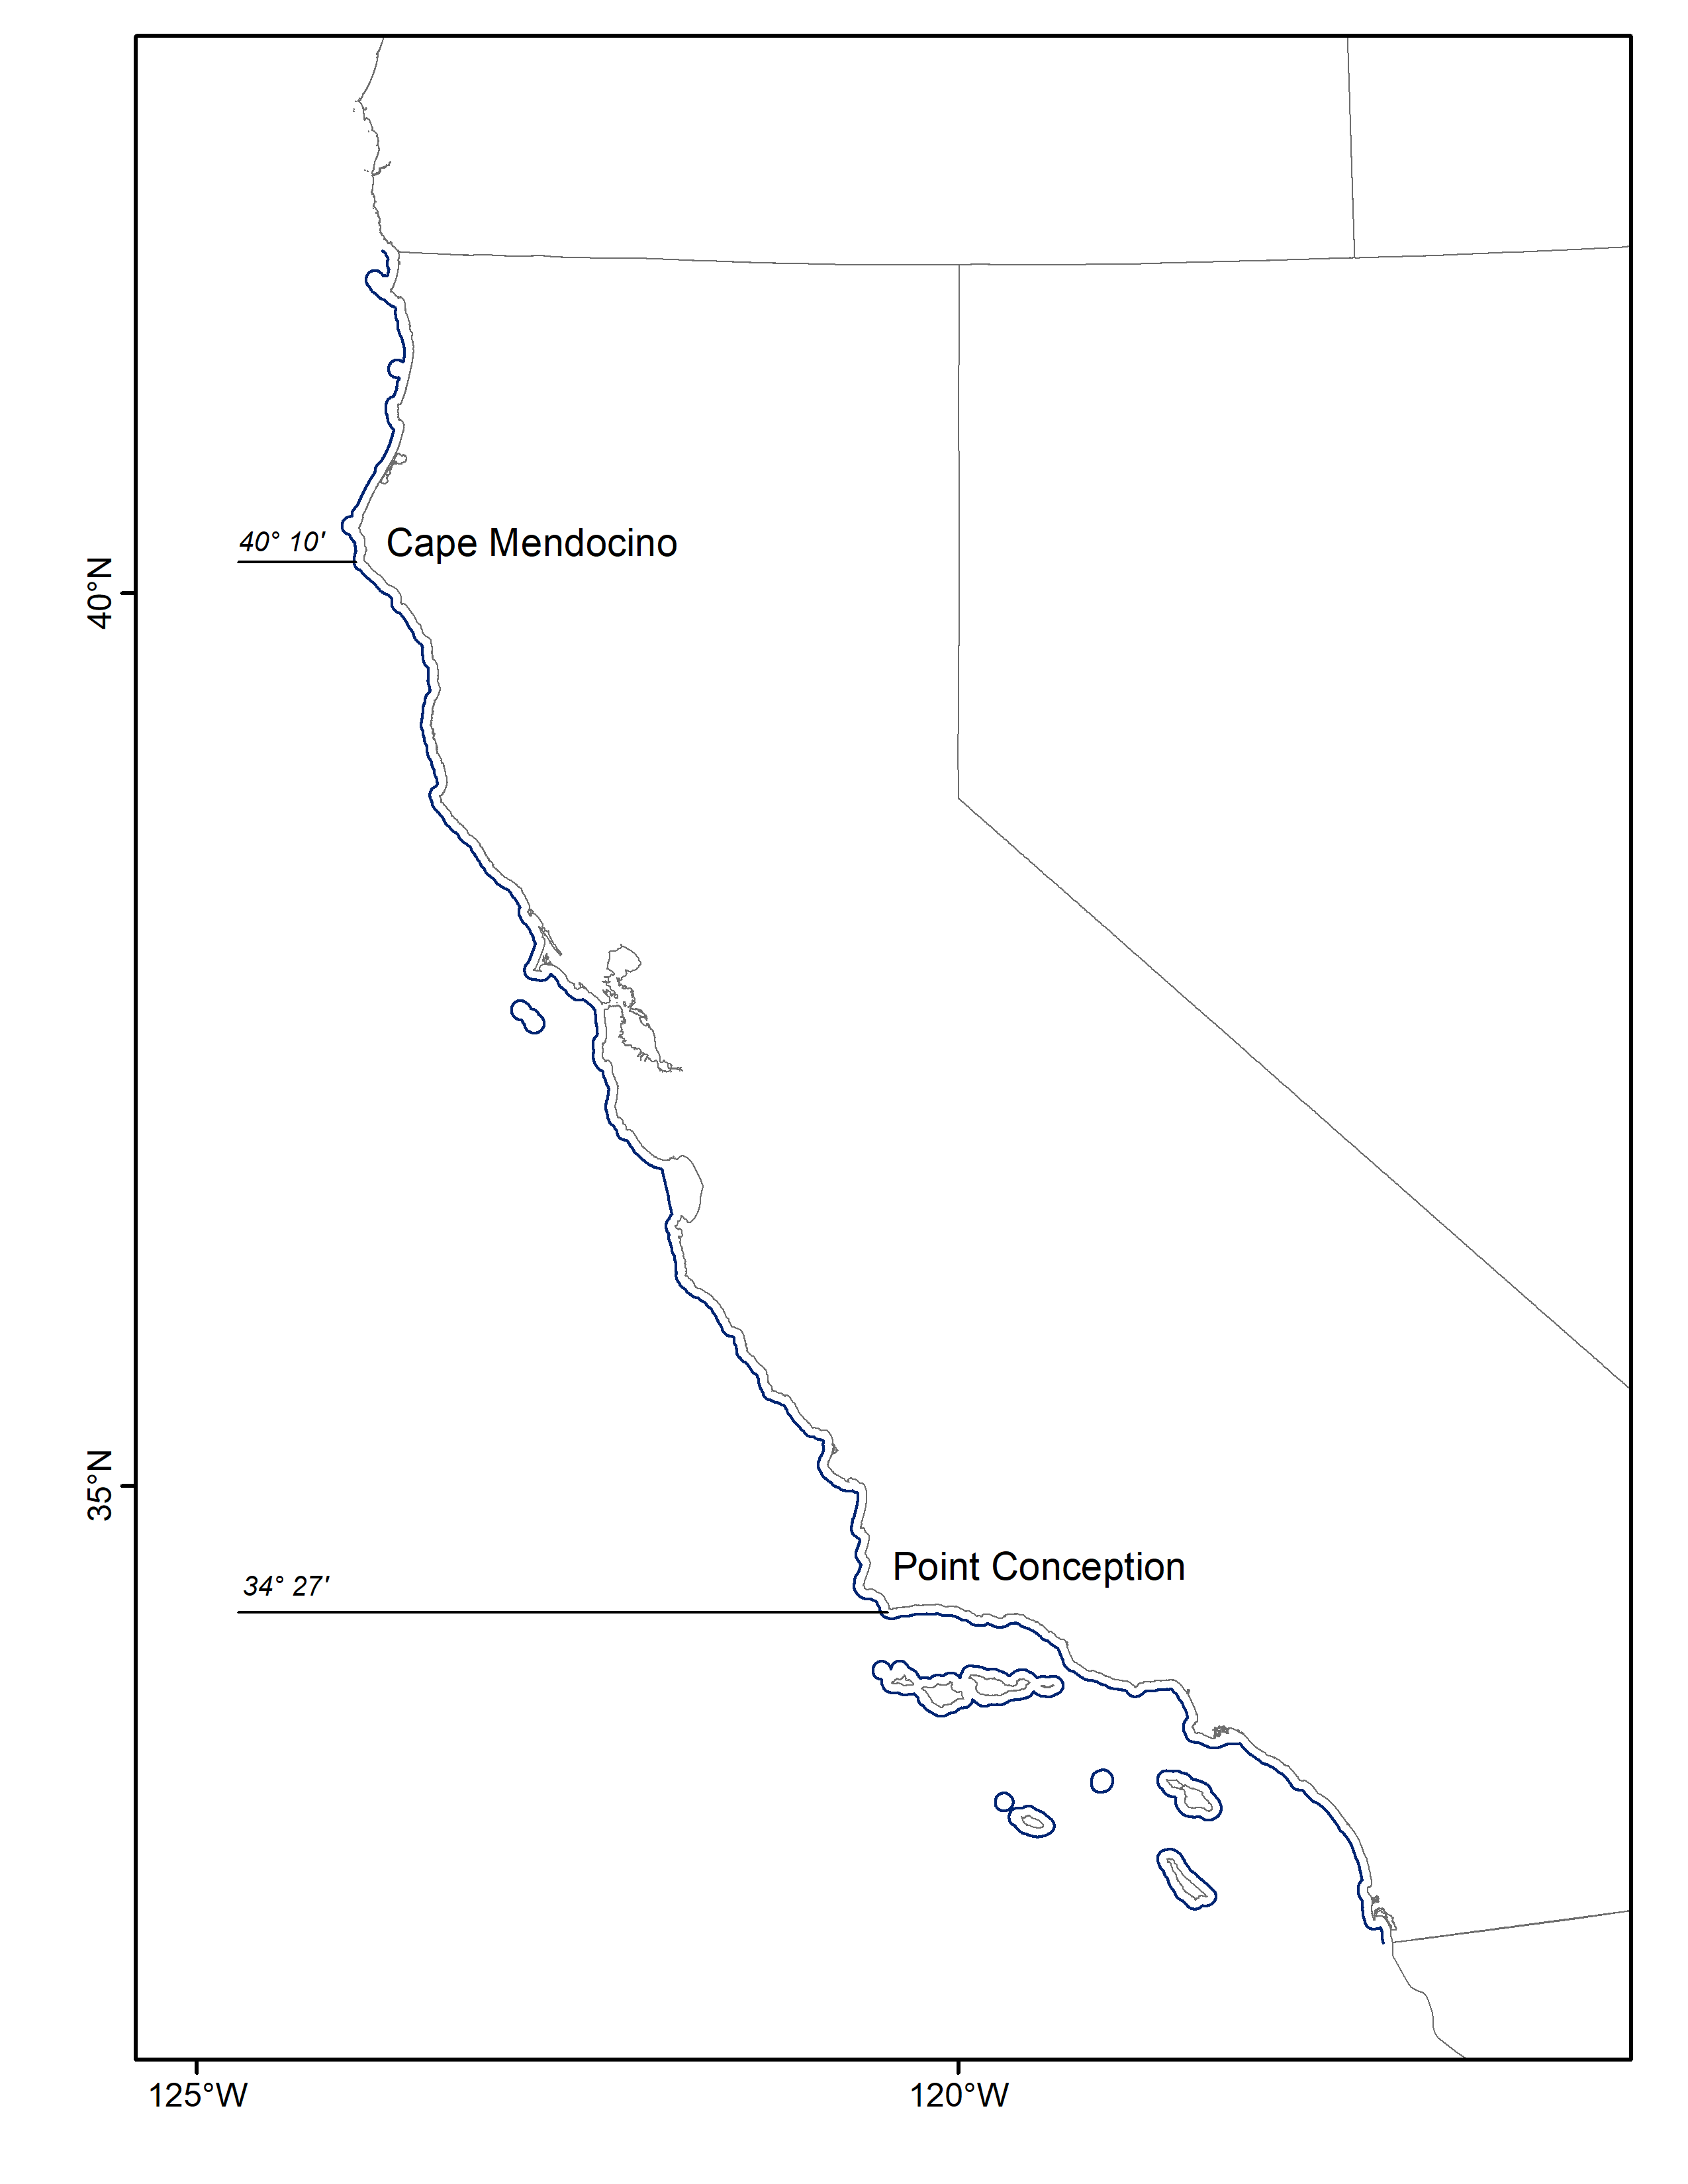
\includegraphics{figures/map.png}

}

\caption{\label{fig-map}An example of the mapped rocky habitat in
California state waters north of Point Conception and an inset of the
state showing the 3 nm state water boundary}

\end{figure}

\begin{figure}

\begin{minipage}[t]{0.50\linewidth}

{\centering 

\raisebox{-\height}{

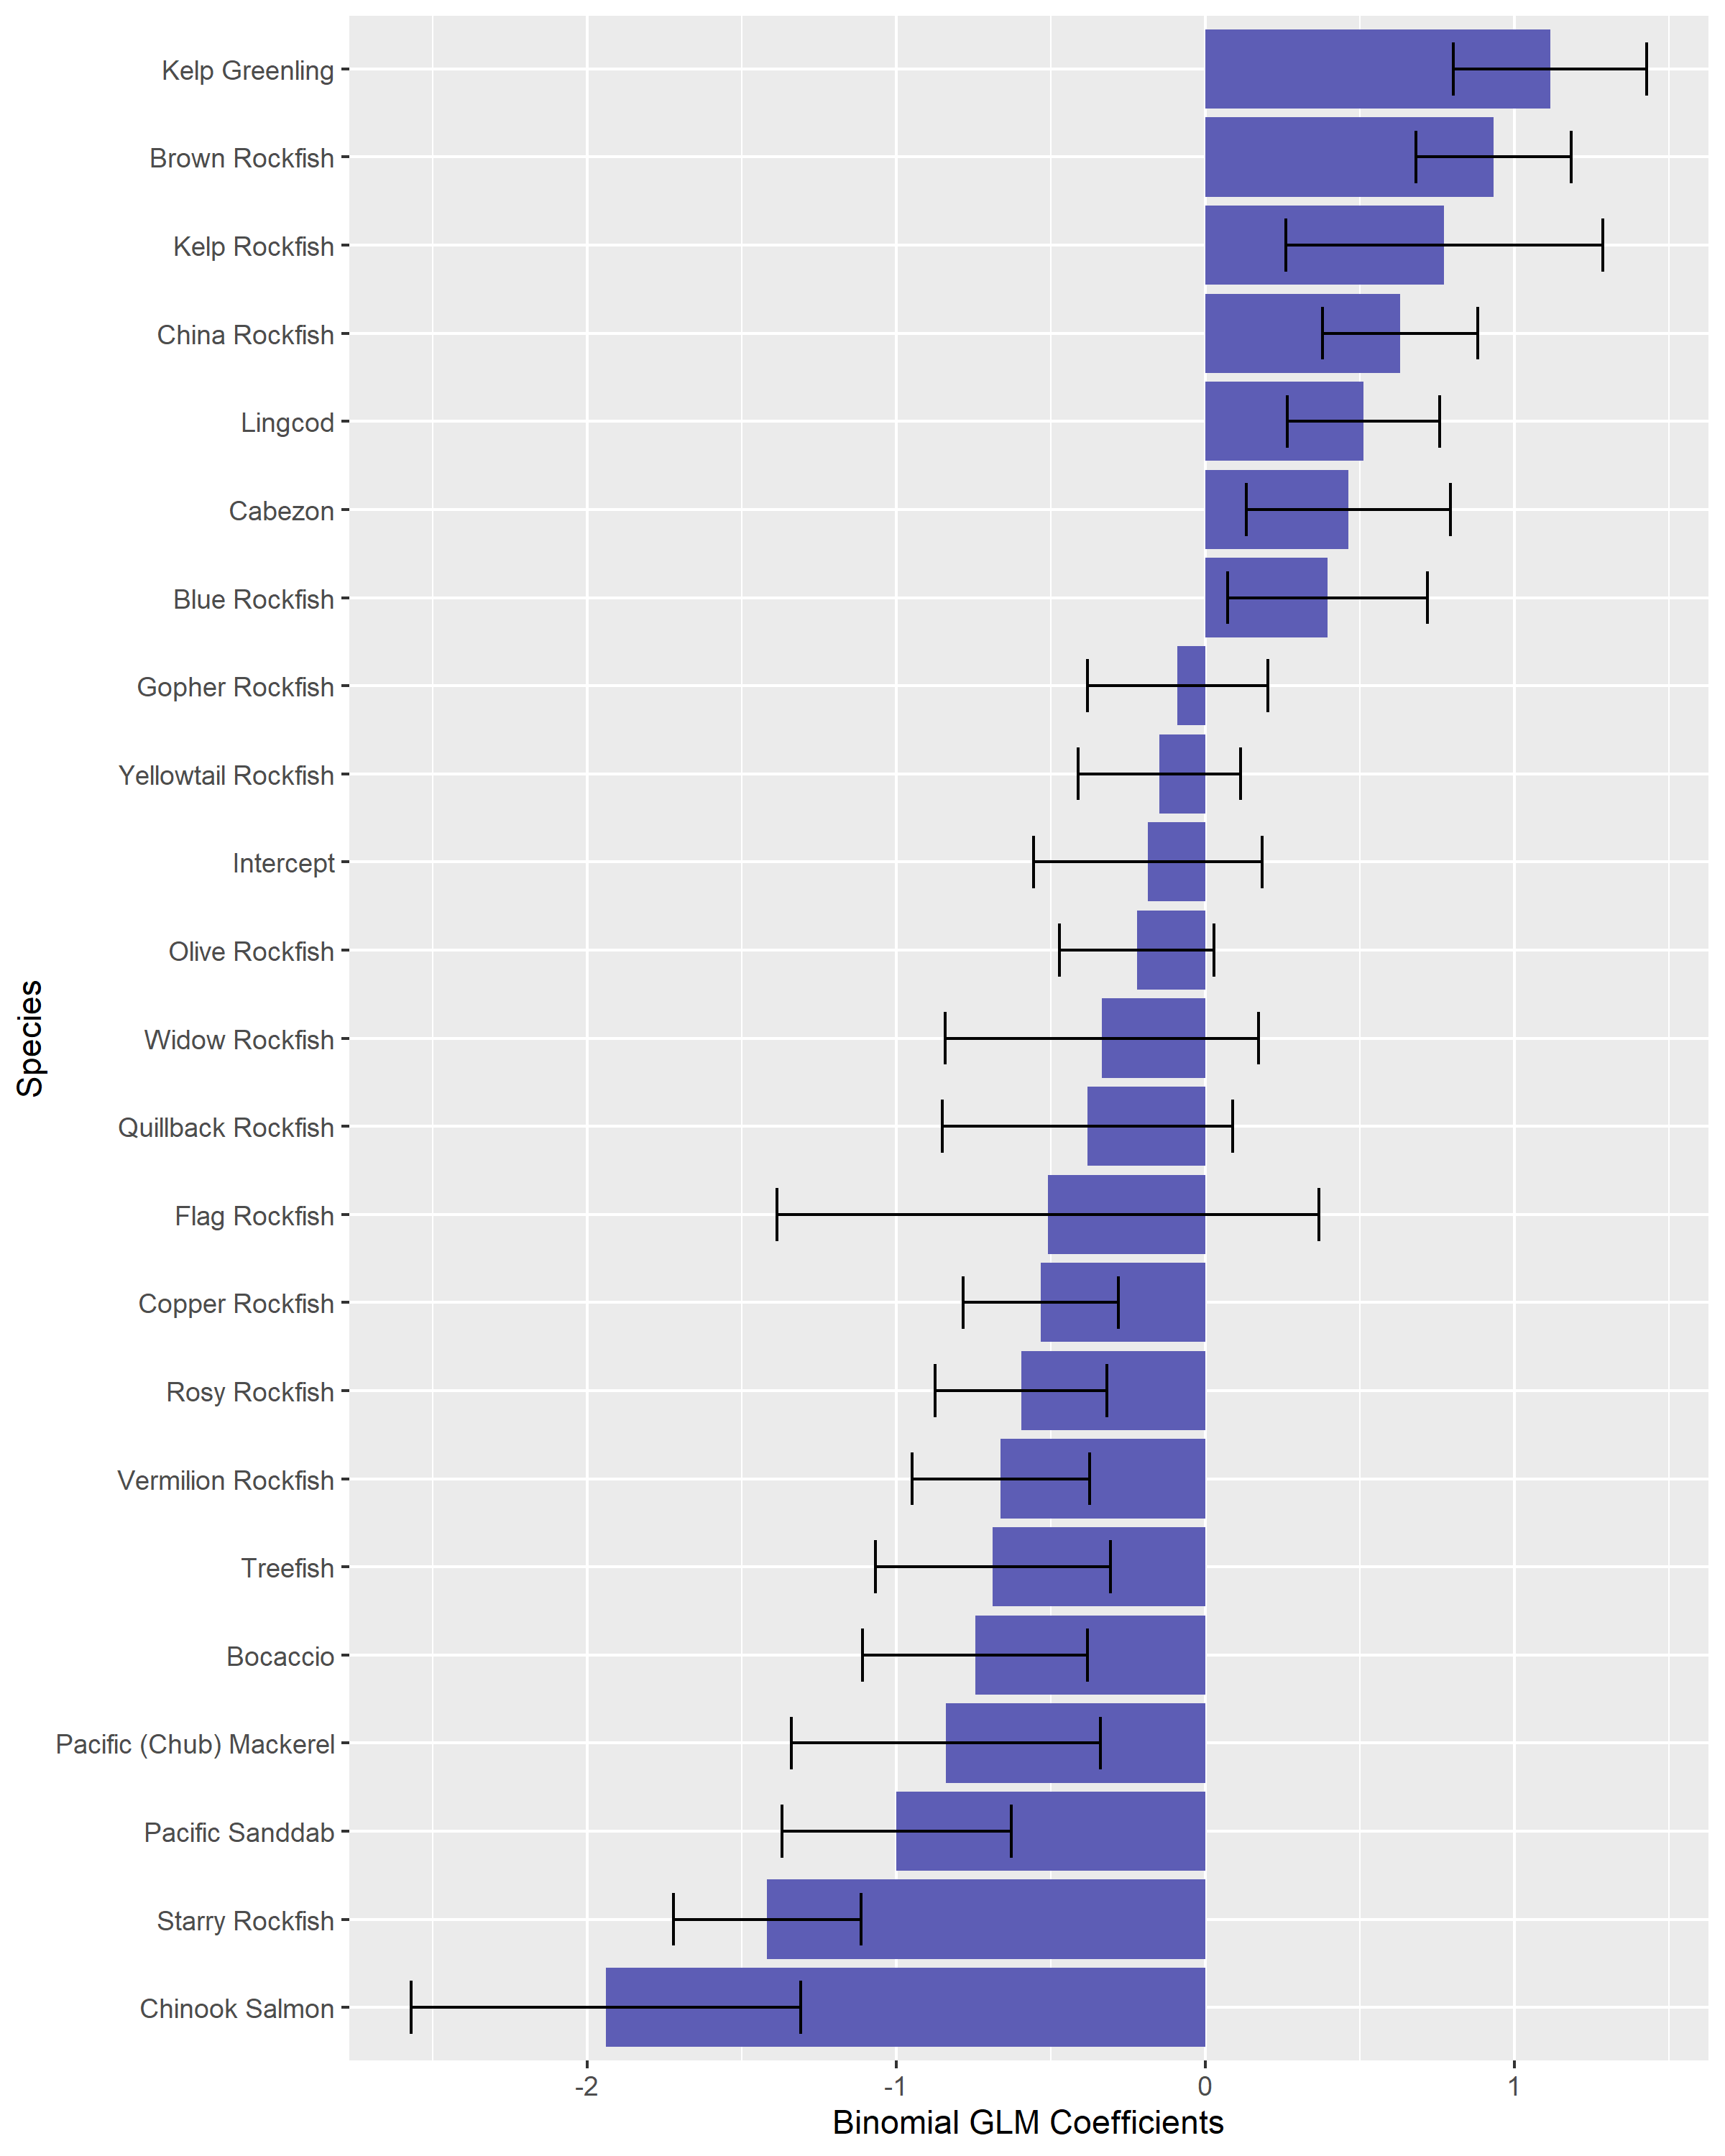
\includegraphics[width=2.75in,height=\textheight]{figures/black_trip_sm.png}

}

}

\subcaption{\label{fig-black-tripsm}Black rockfish trip level}
\end{minipage}%
%
\begin{minipage}[t]{0.50\linewidth}

{\centering 

\raisebox{-\height}{

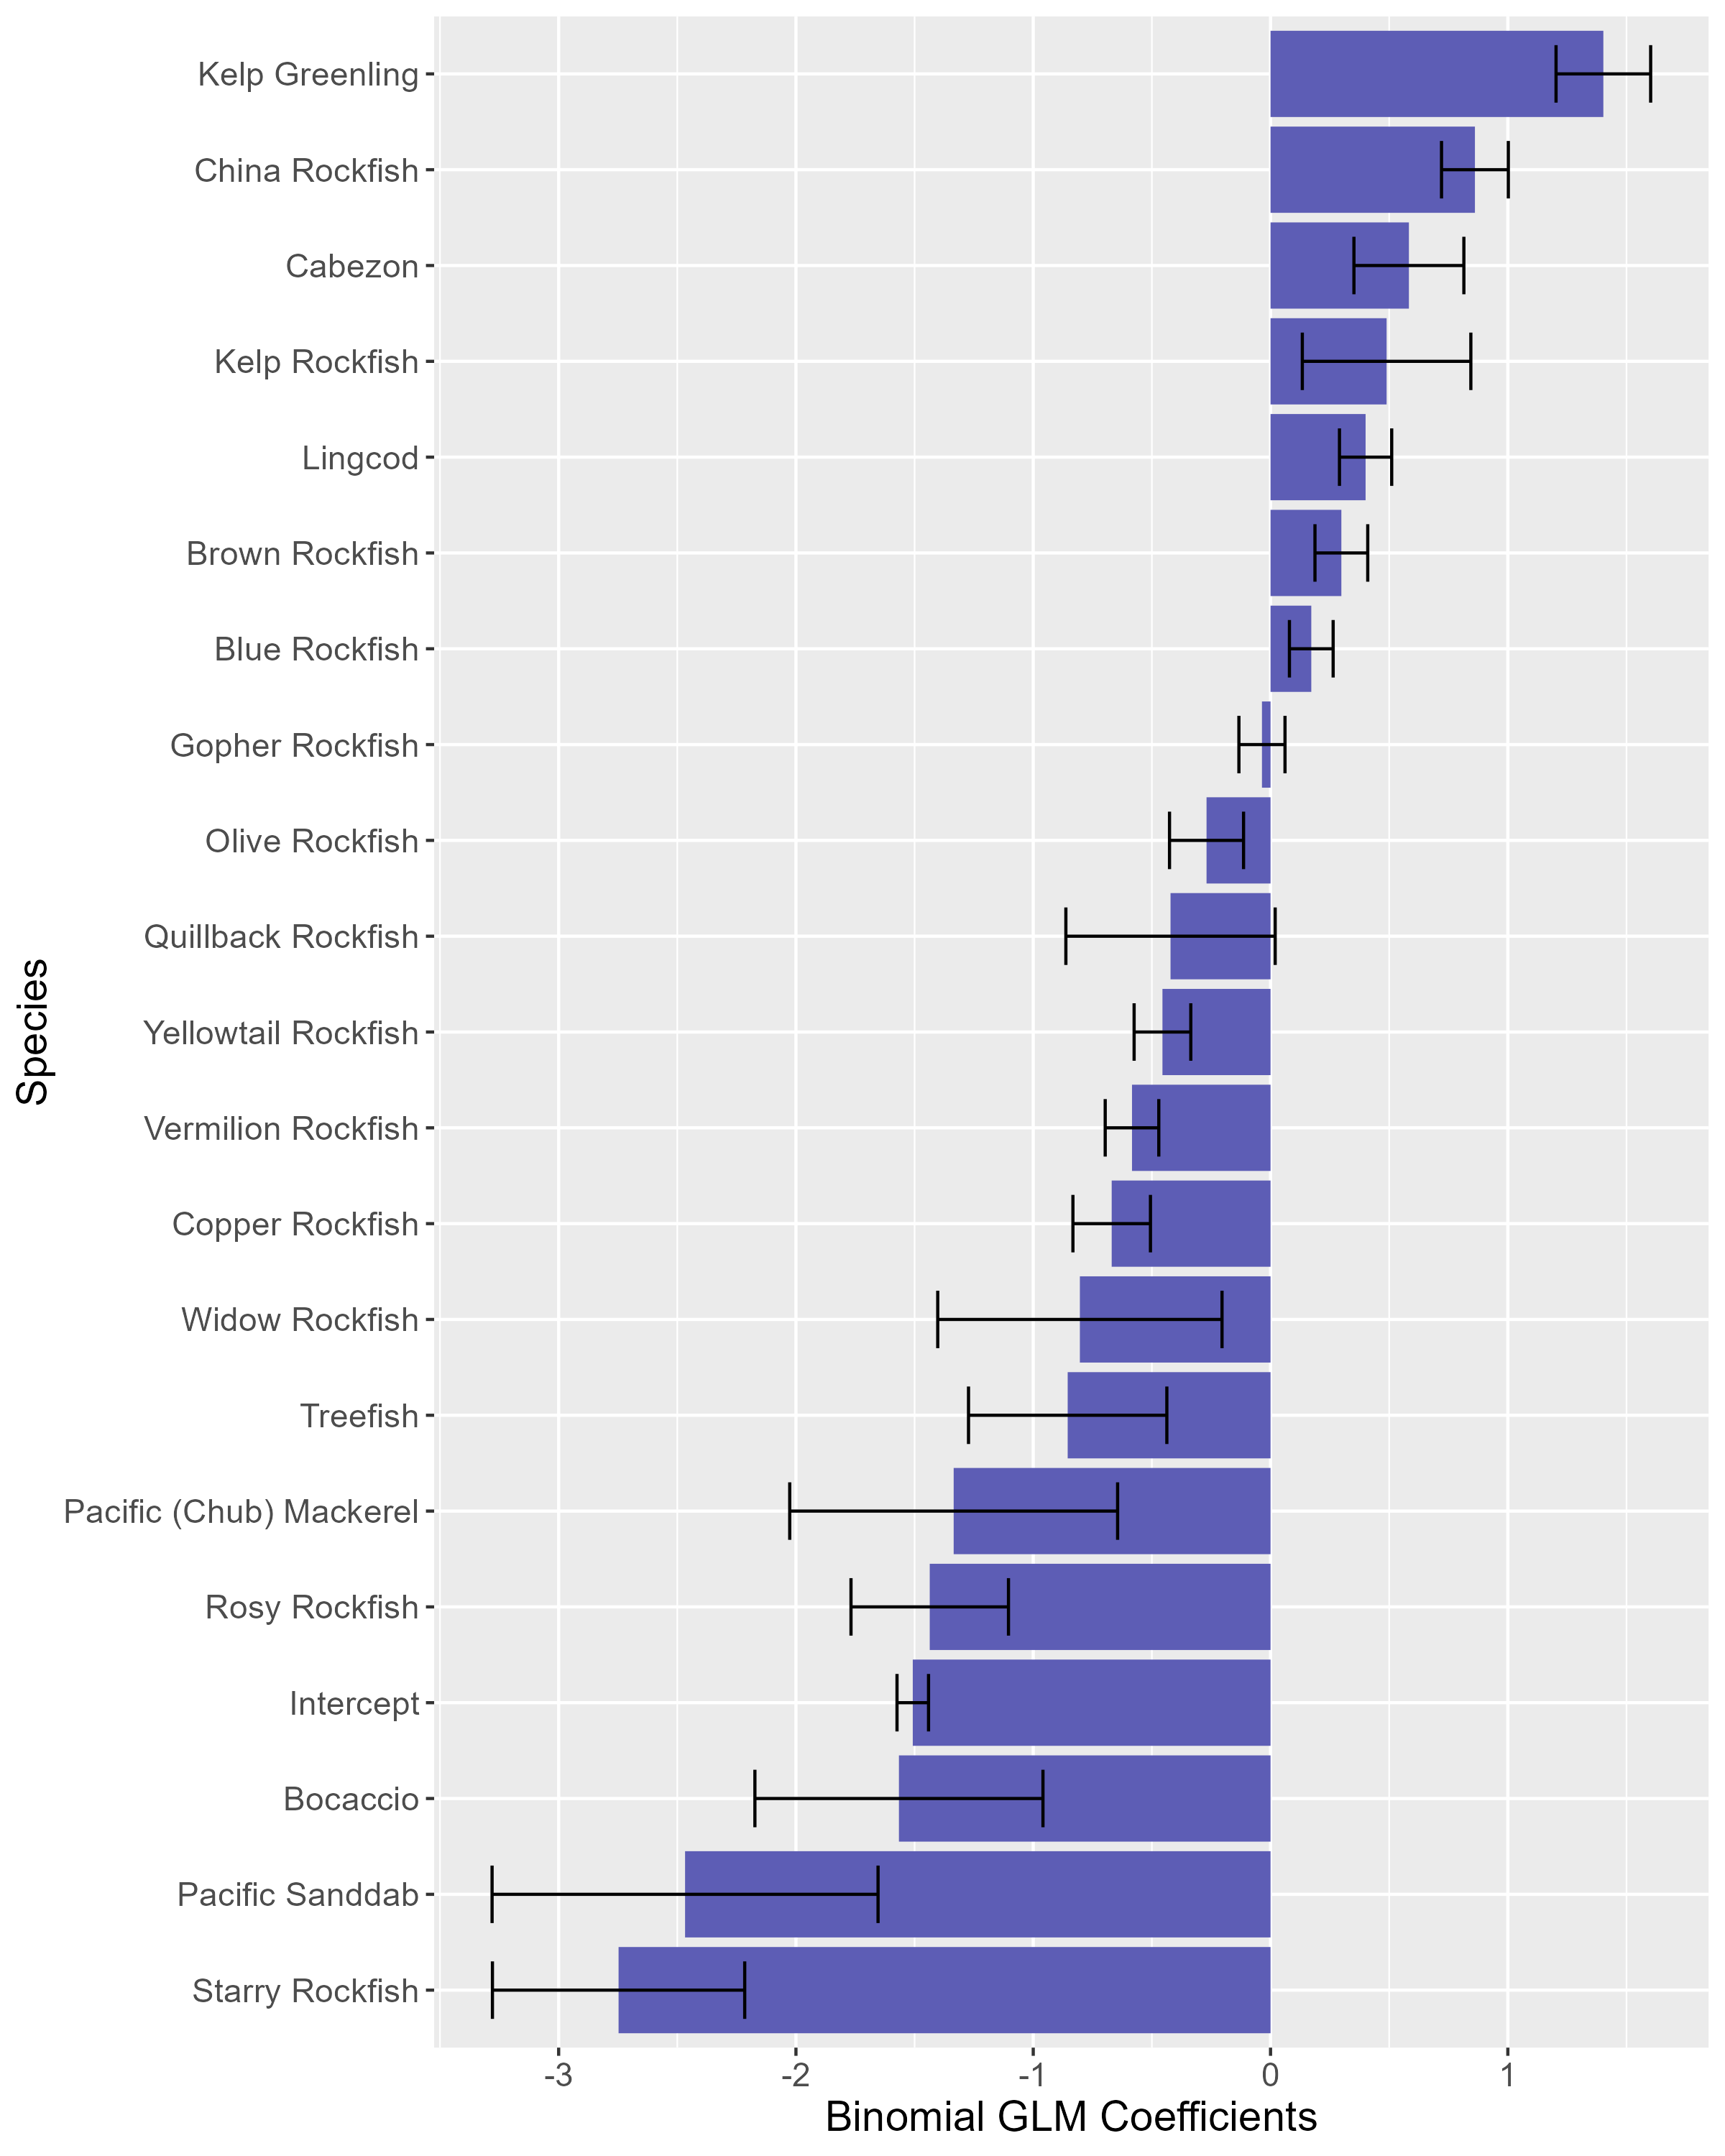
\includegraphics[width=2.75in,height=\textheight]{figures/black_drift_sm.png}

}

}

\subcaption{\label{fig-black-driftsm}Black rockfish drift level}
\end{minipage}%
\newline
\begin{minipage}[t]{0.52\linewidth}

{\centering 

\raisebox{-\height}{

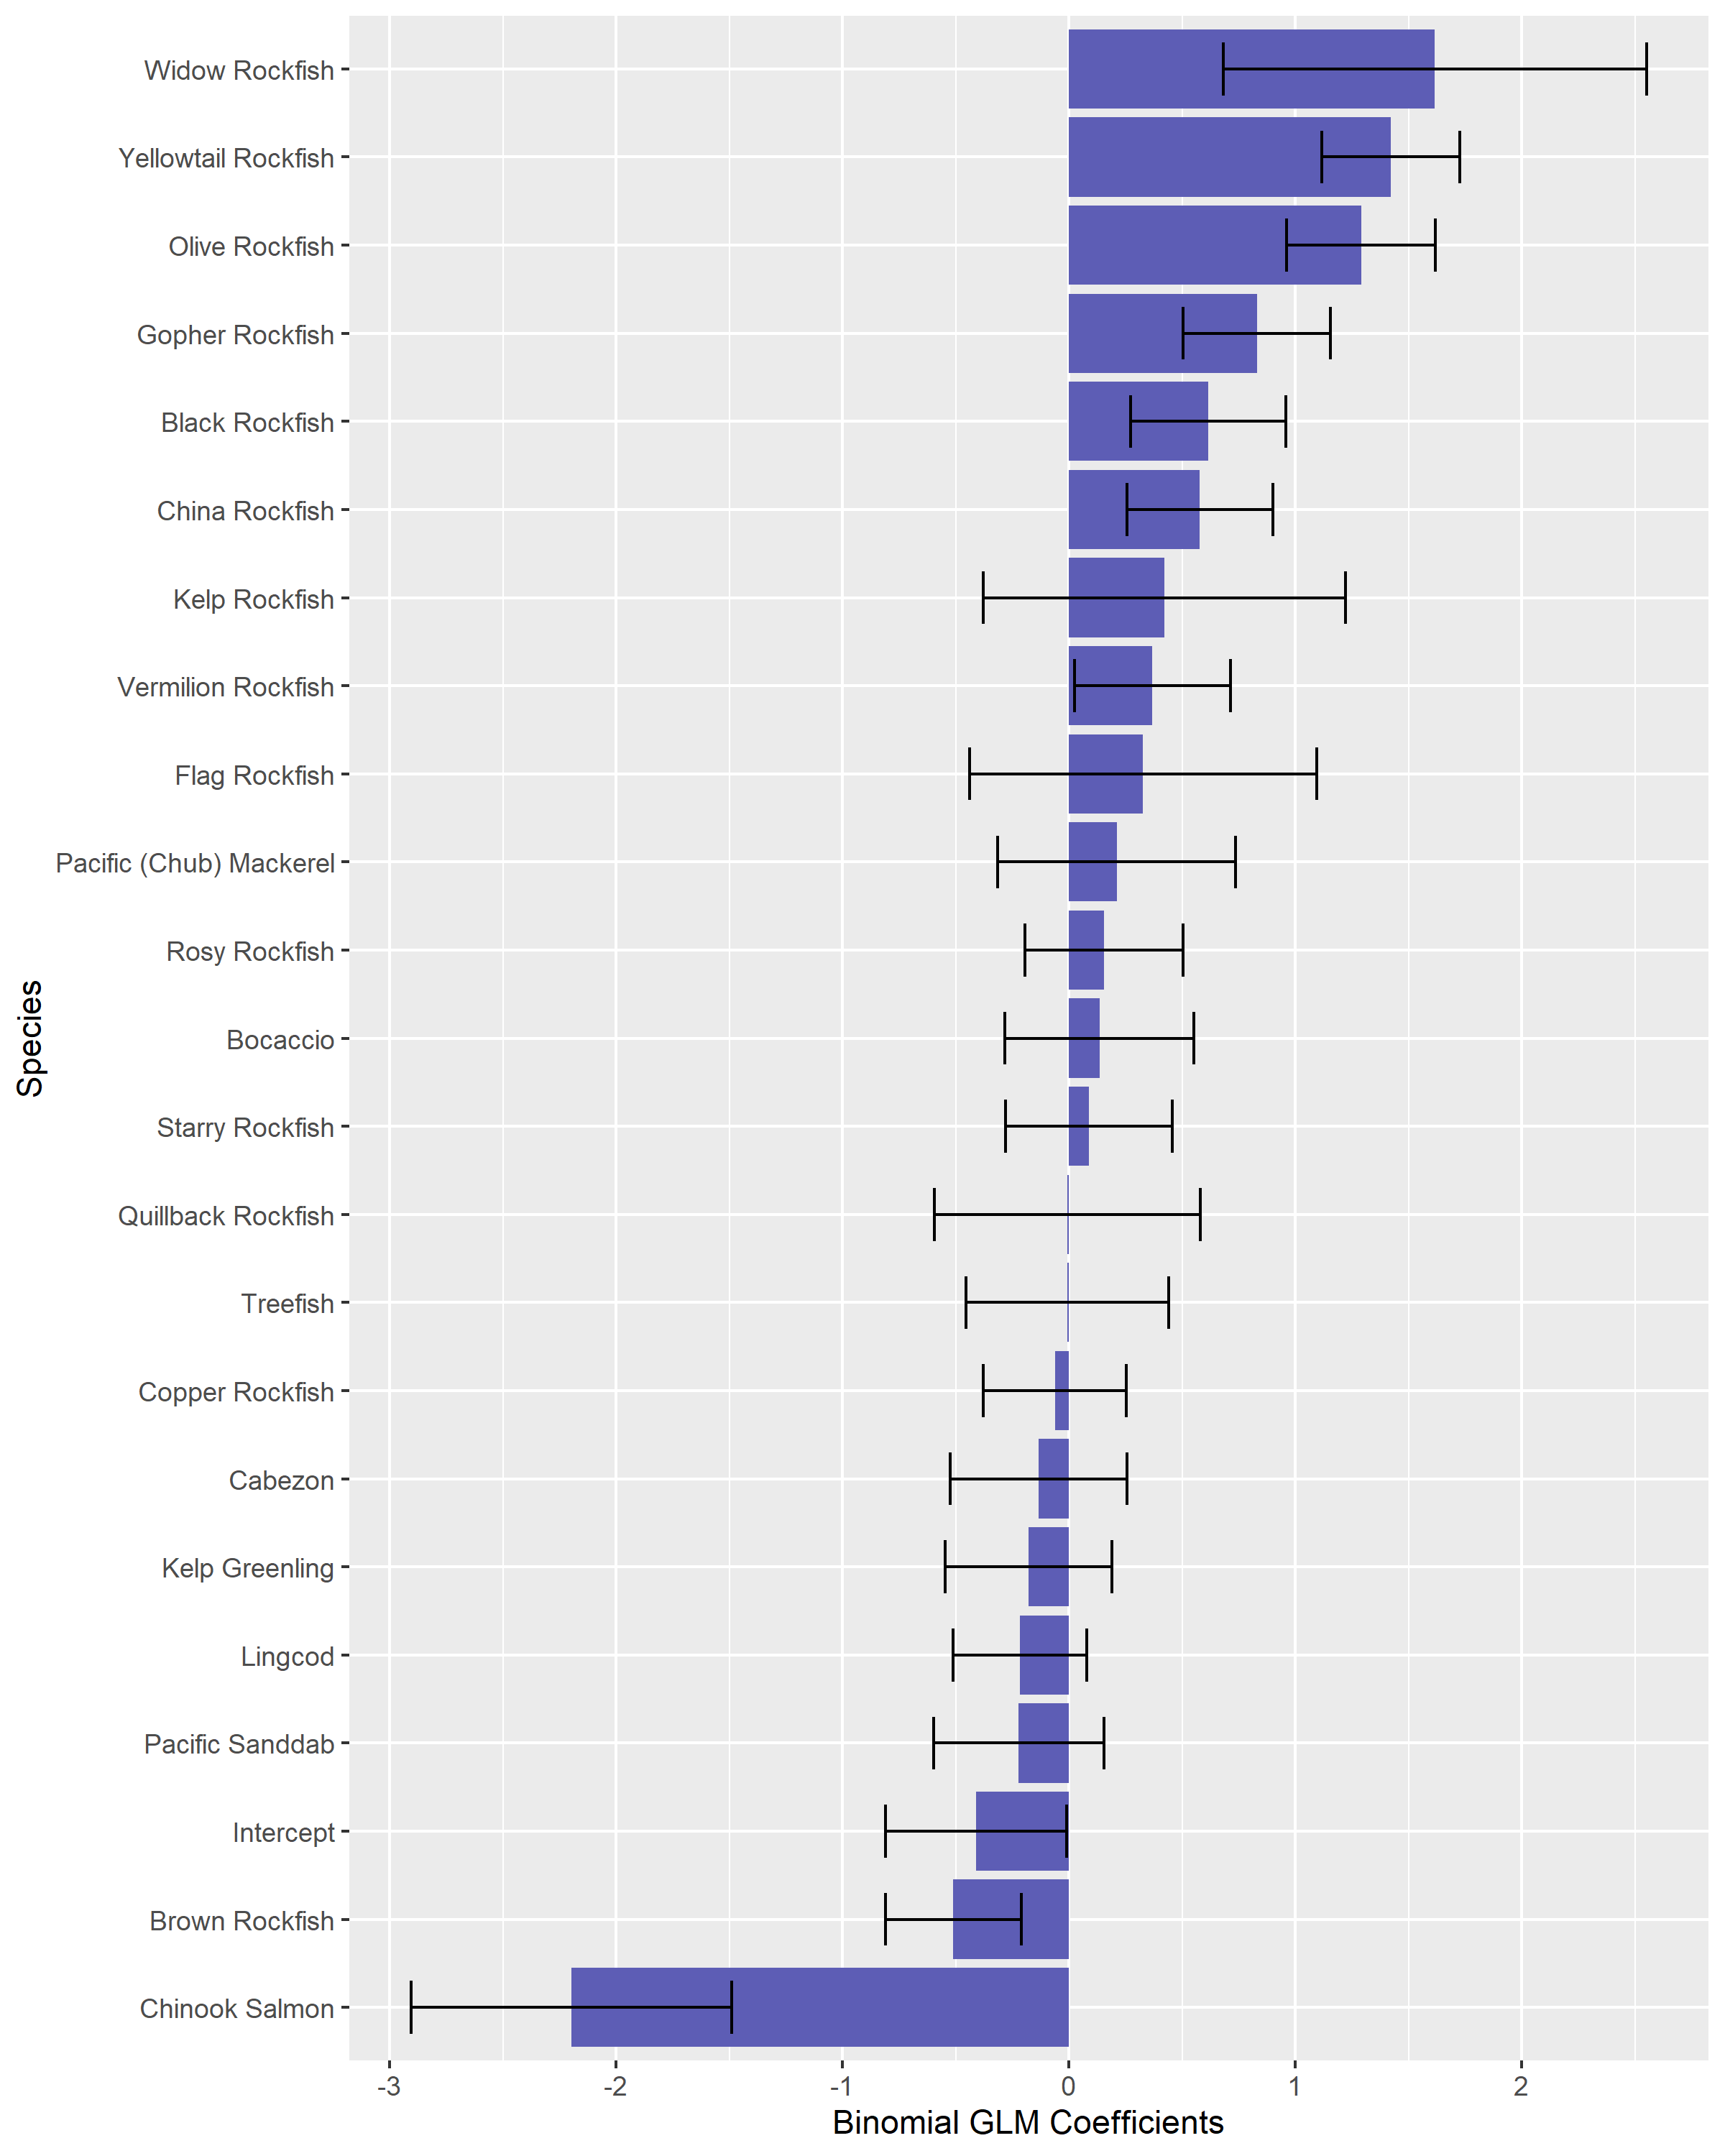
\includegraphics[width=0.03125in,height=\textheight]{figures/blue_trip_sm.png}

}

}

\subcaption{\label{fig-blue-tripsm}Blue rockfish trip level}
\end{minipage}%
%
\begin{minipage}[t]{0.48\linewidth}

{\centering 

\raisebox{-\height}{

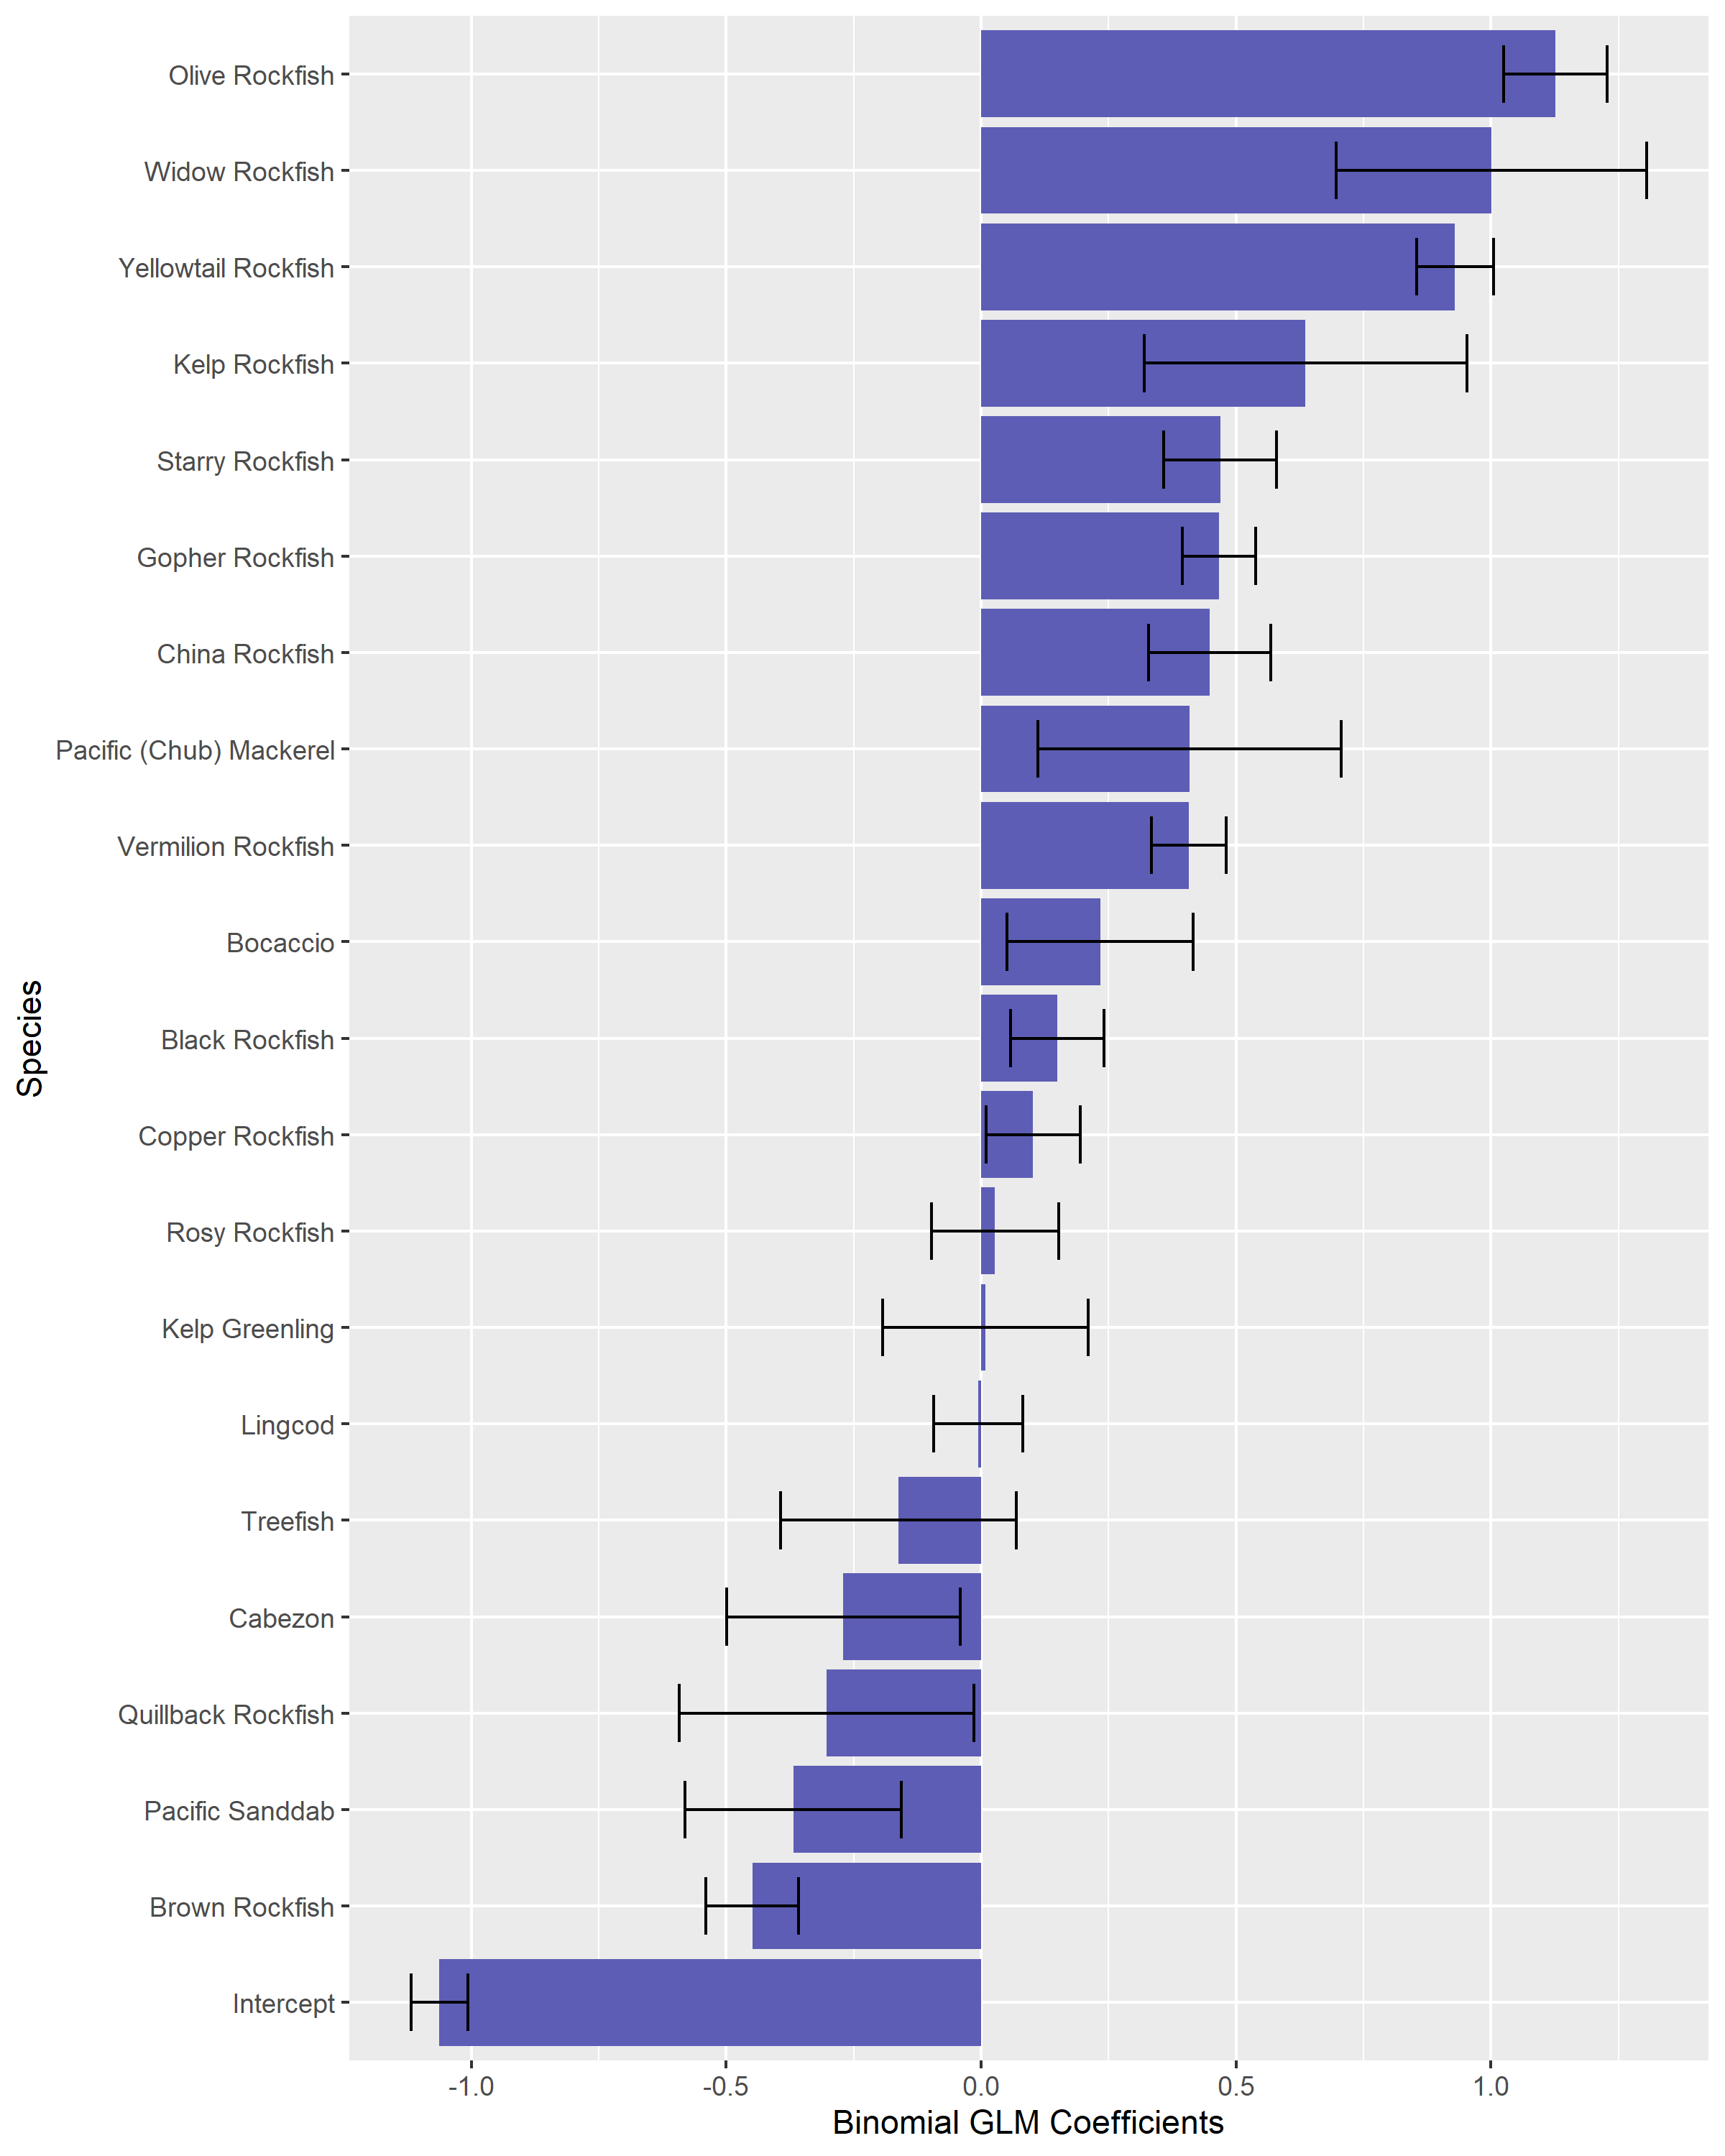
\includegraphics[width=2.75in,height=\textheight]{figures/blue_drift_sm.png}

}

}

\subcaption{\label{fig-blue-driftsm}Blue rockfish drift level}
\end{minipage}%

\caption{\label{fig-sm}SM figure 1}

\end{figure}

\begin{figure}

\begin{minipage}[t]{0.50\linewidth}

{\centering 

\raisebox{-\height}{

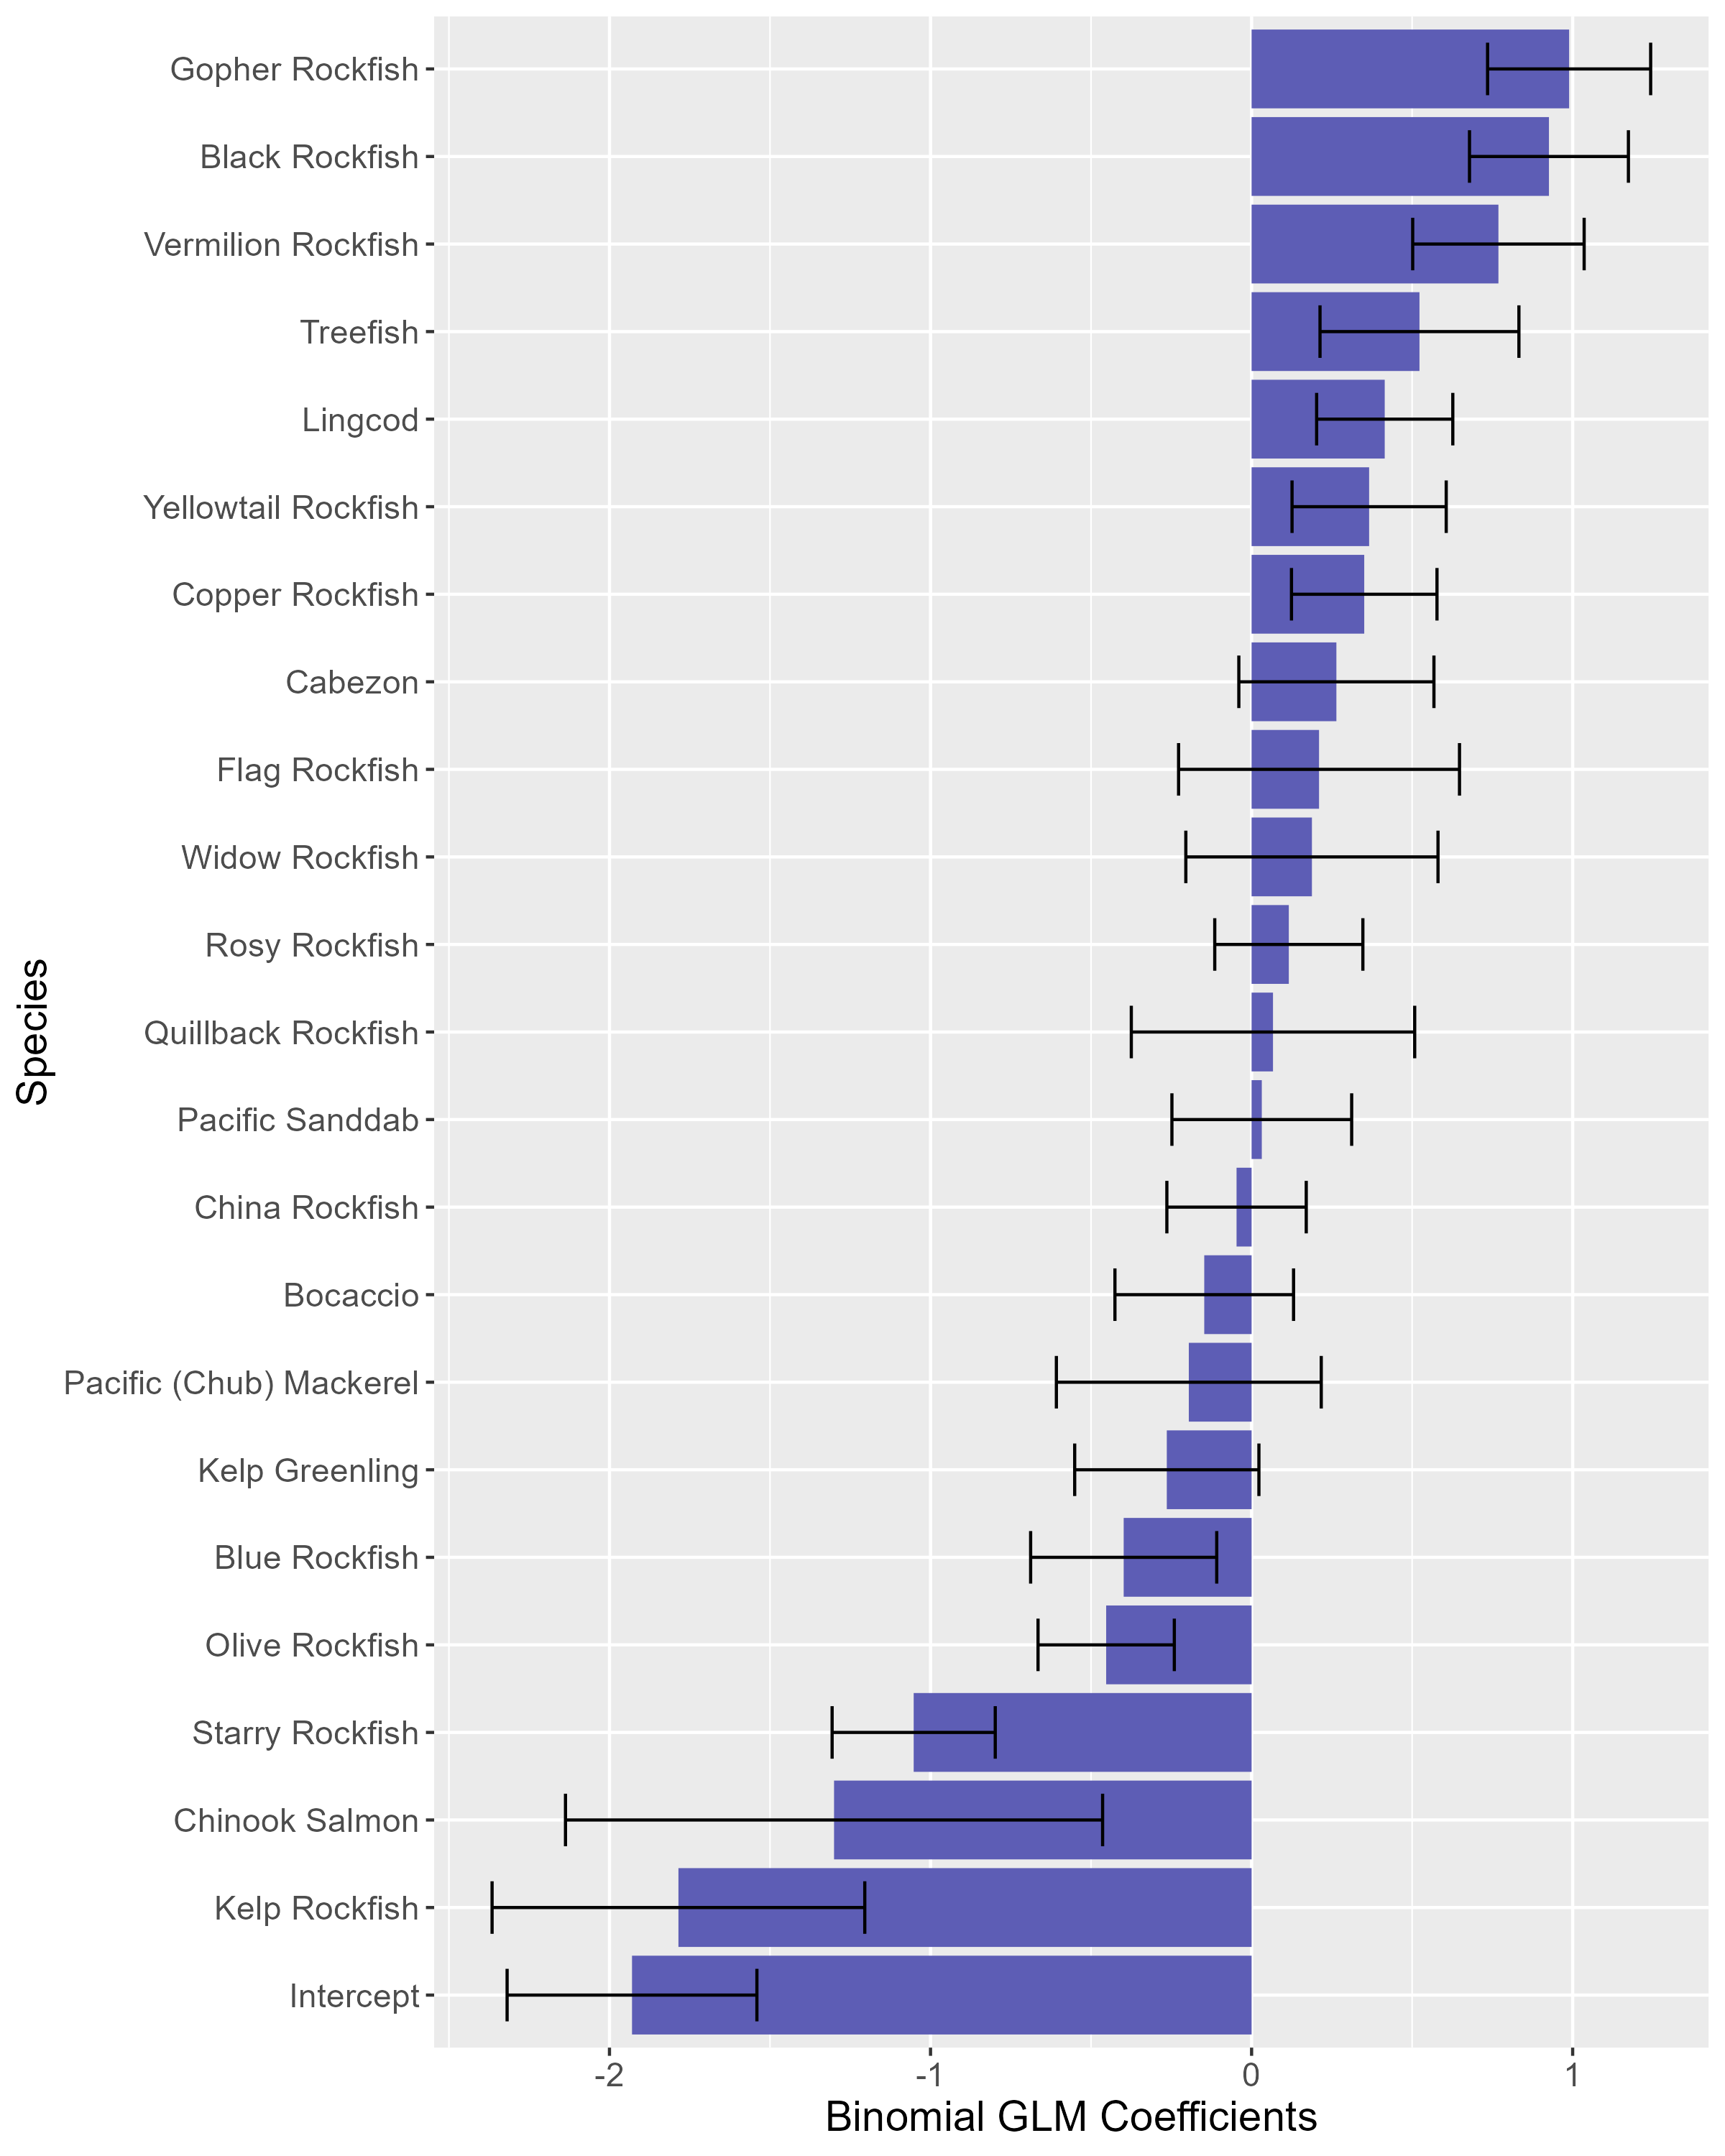
\includegraphics[width=2.75in,height=\textheight]{figures/brown_trip_sm.png}

}

}

\subcaption{\label{fig-brown-tripsm}Brown rockfish trip level}
\end{minipage}%
%
\begin{minipage}[t]{0.50\linewidth}

{\centering 

\raisebox{-\height}{

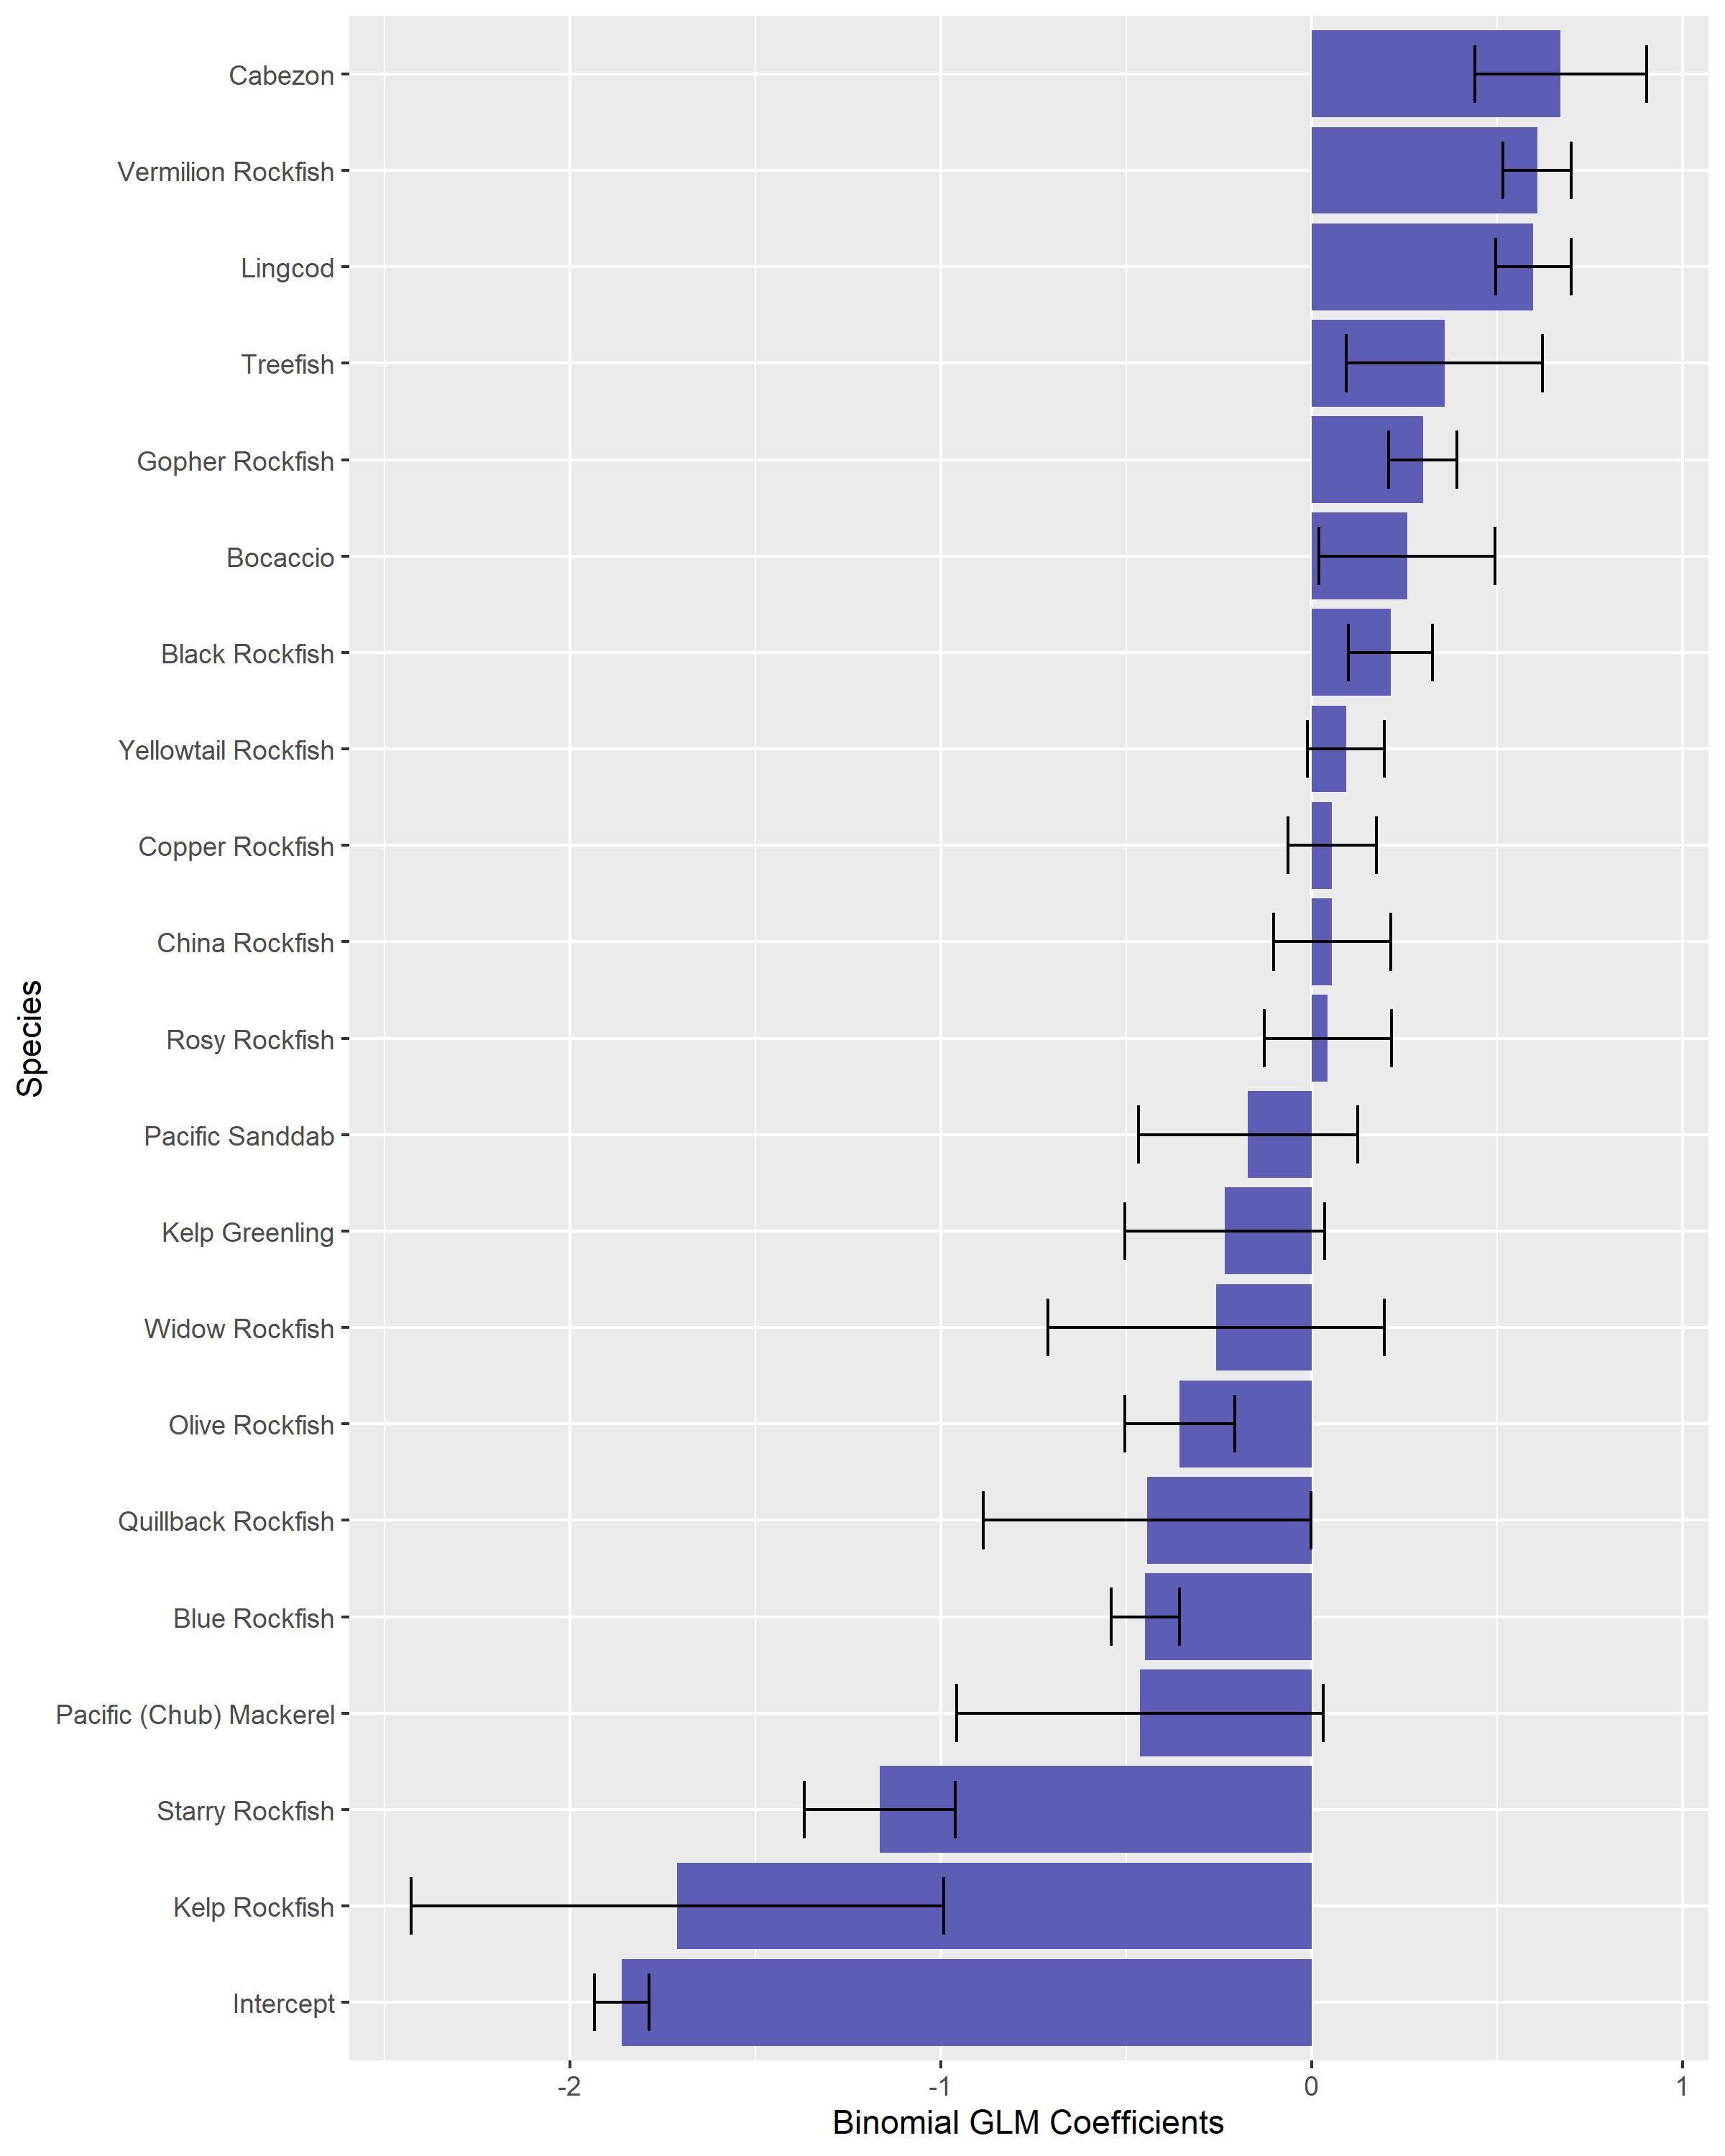
\includegraphics[width=2.75in,height=\textheight]{figures/brown_drift_sm.png}

}

}

\subcaption{\label{fig-brown-driftsm}Brown rockfish drift level}
\end{minipage}%
\newline
\begin{minipage}[t]{0.50\linewidth}

{\centering 

\raisebox{-\height}{

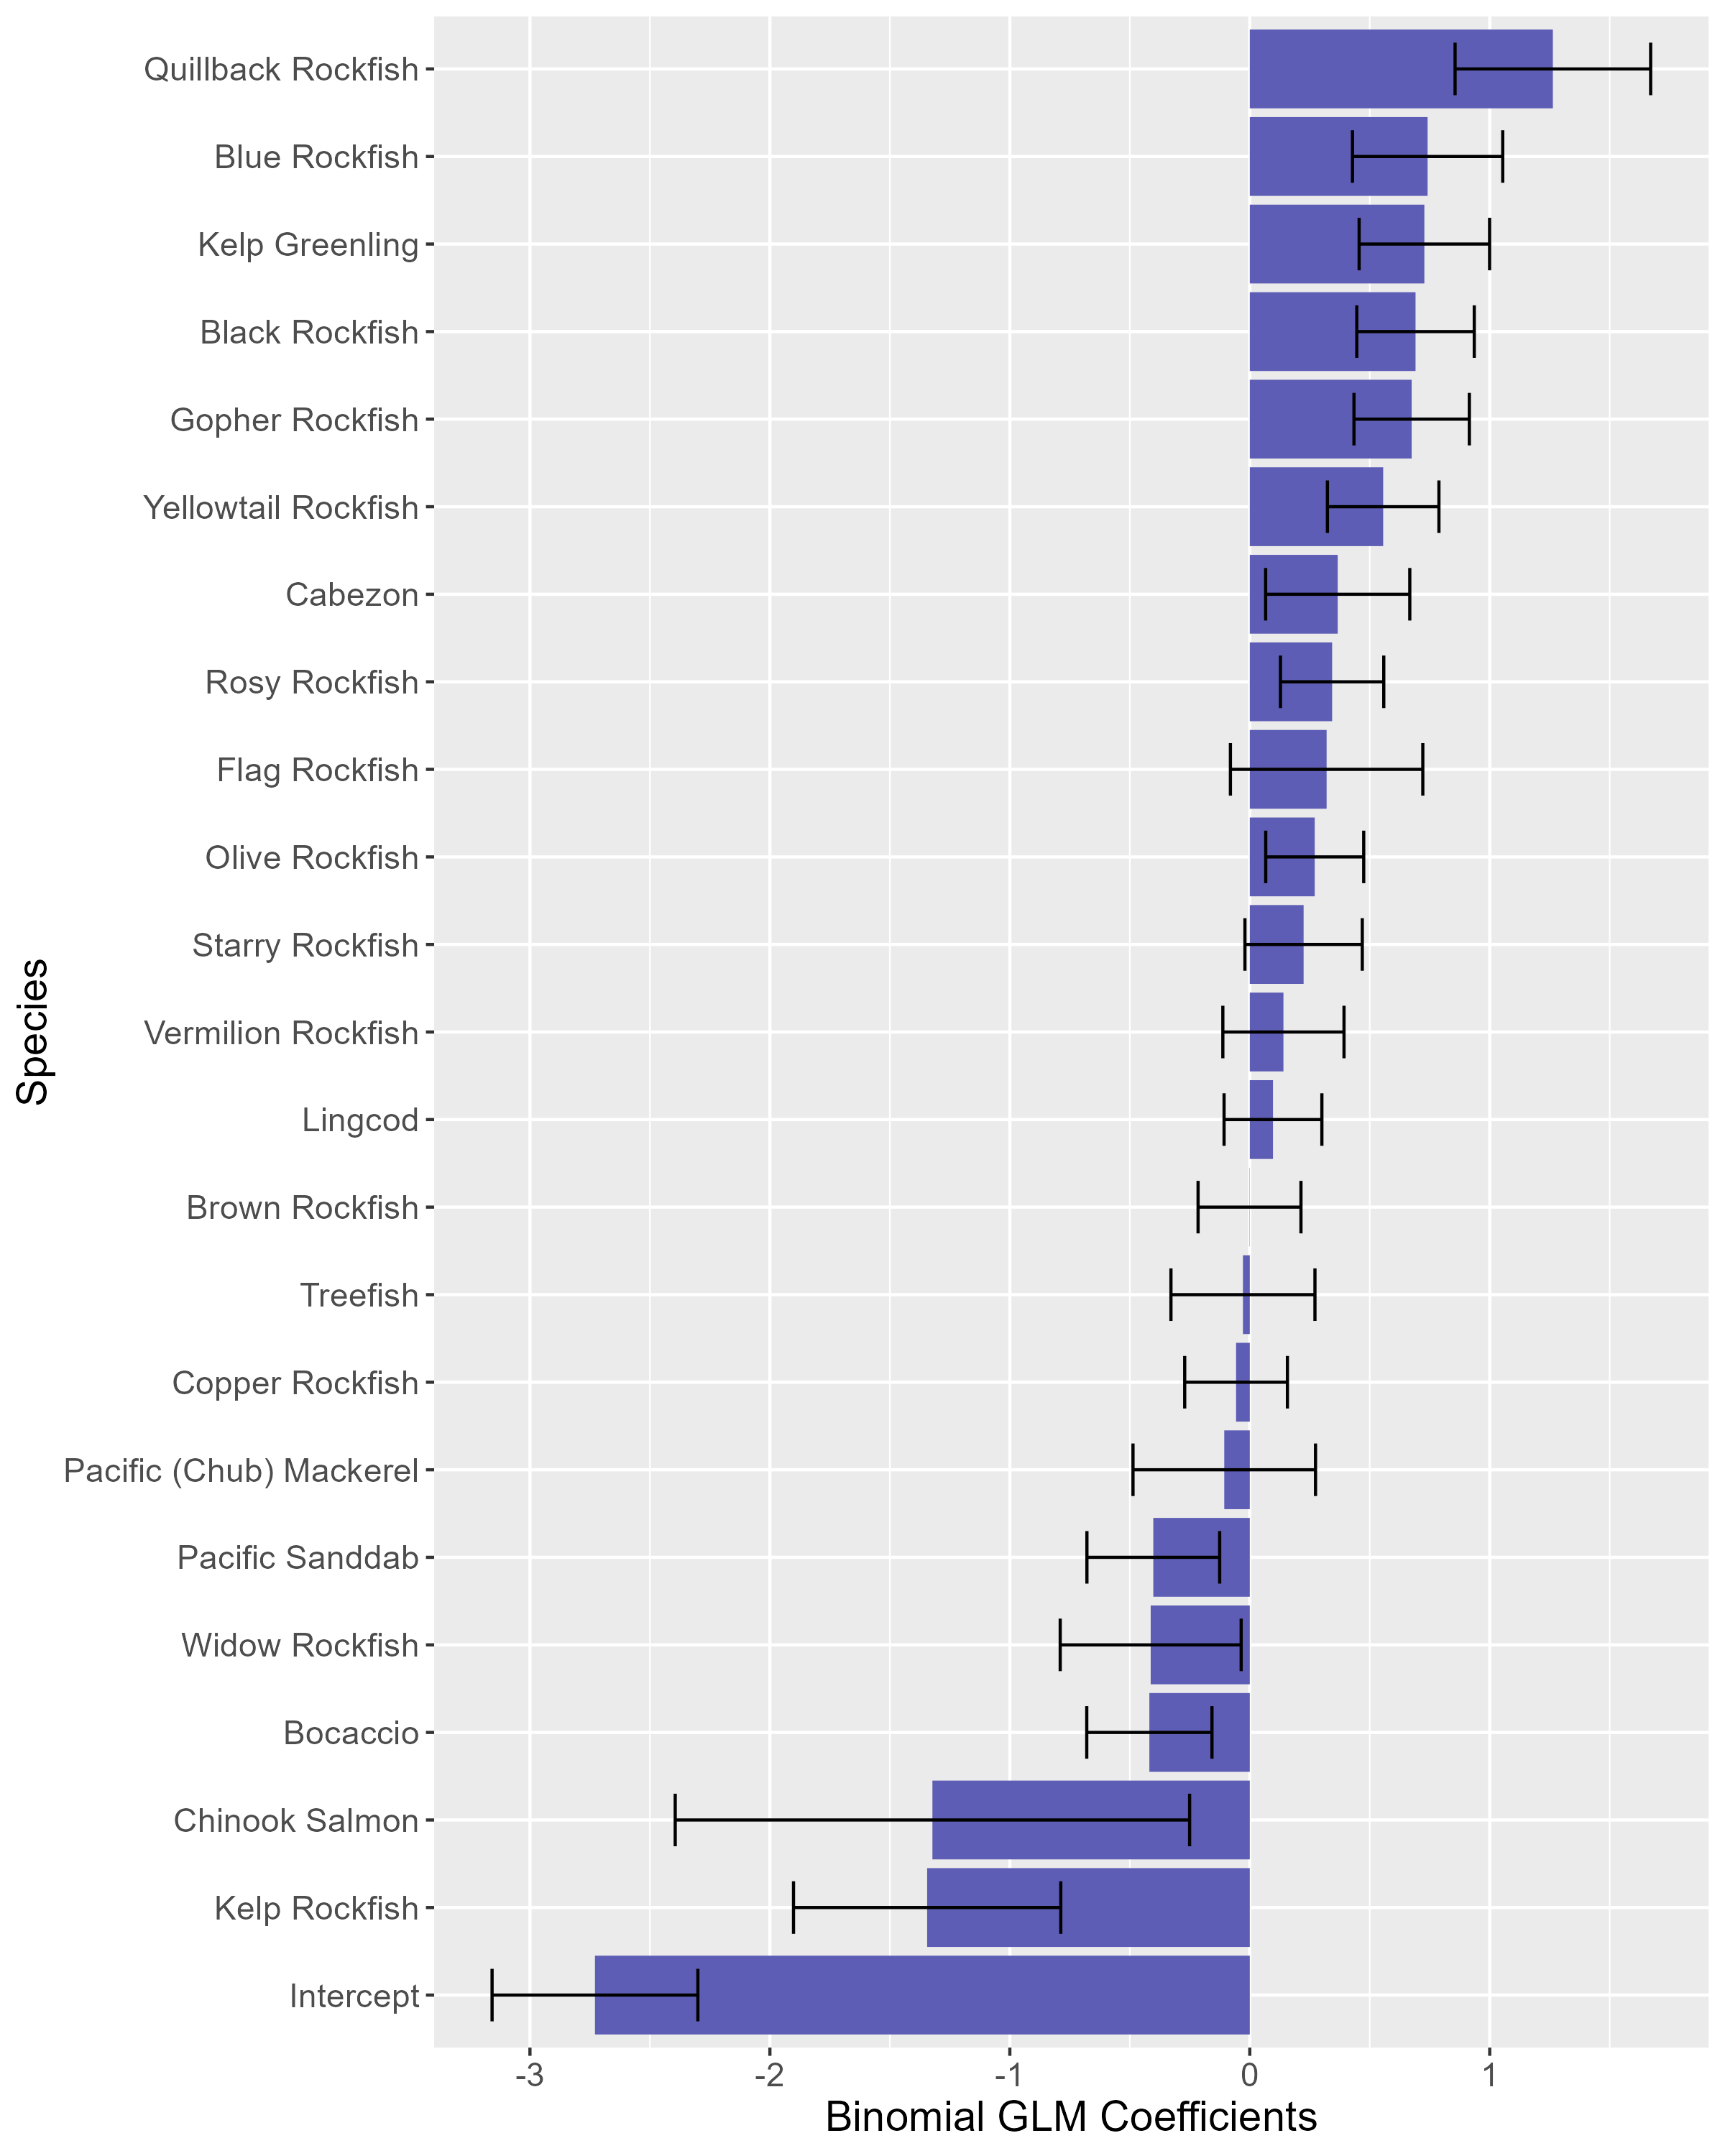
\includegraphics[width=2.75in,height=\textheight]{figures/china_trip_sm.png}

}

}

\subcaption{\label{fig-china-tripsm}China rockfish trip level}
\end{minipage}%
%
\begin{minipage}[t]{0.50\linewidth}

{\centering 

\raisebox{-\height}{

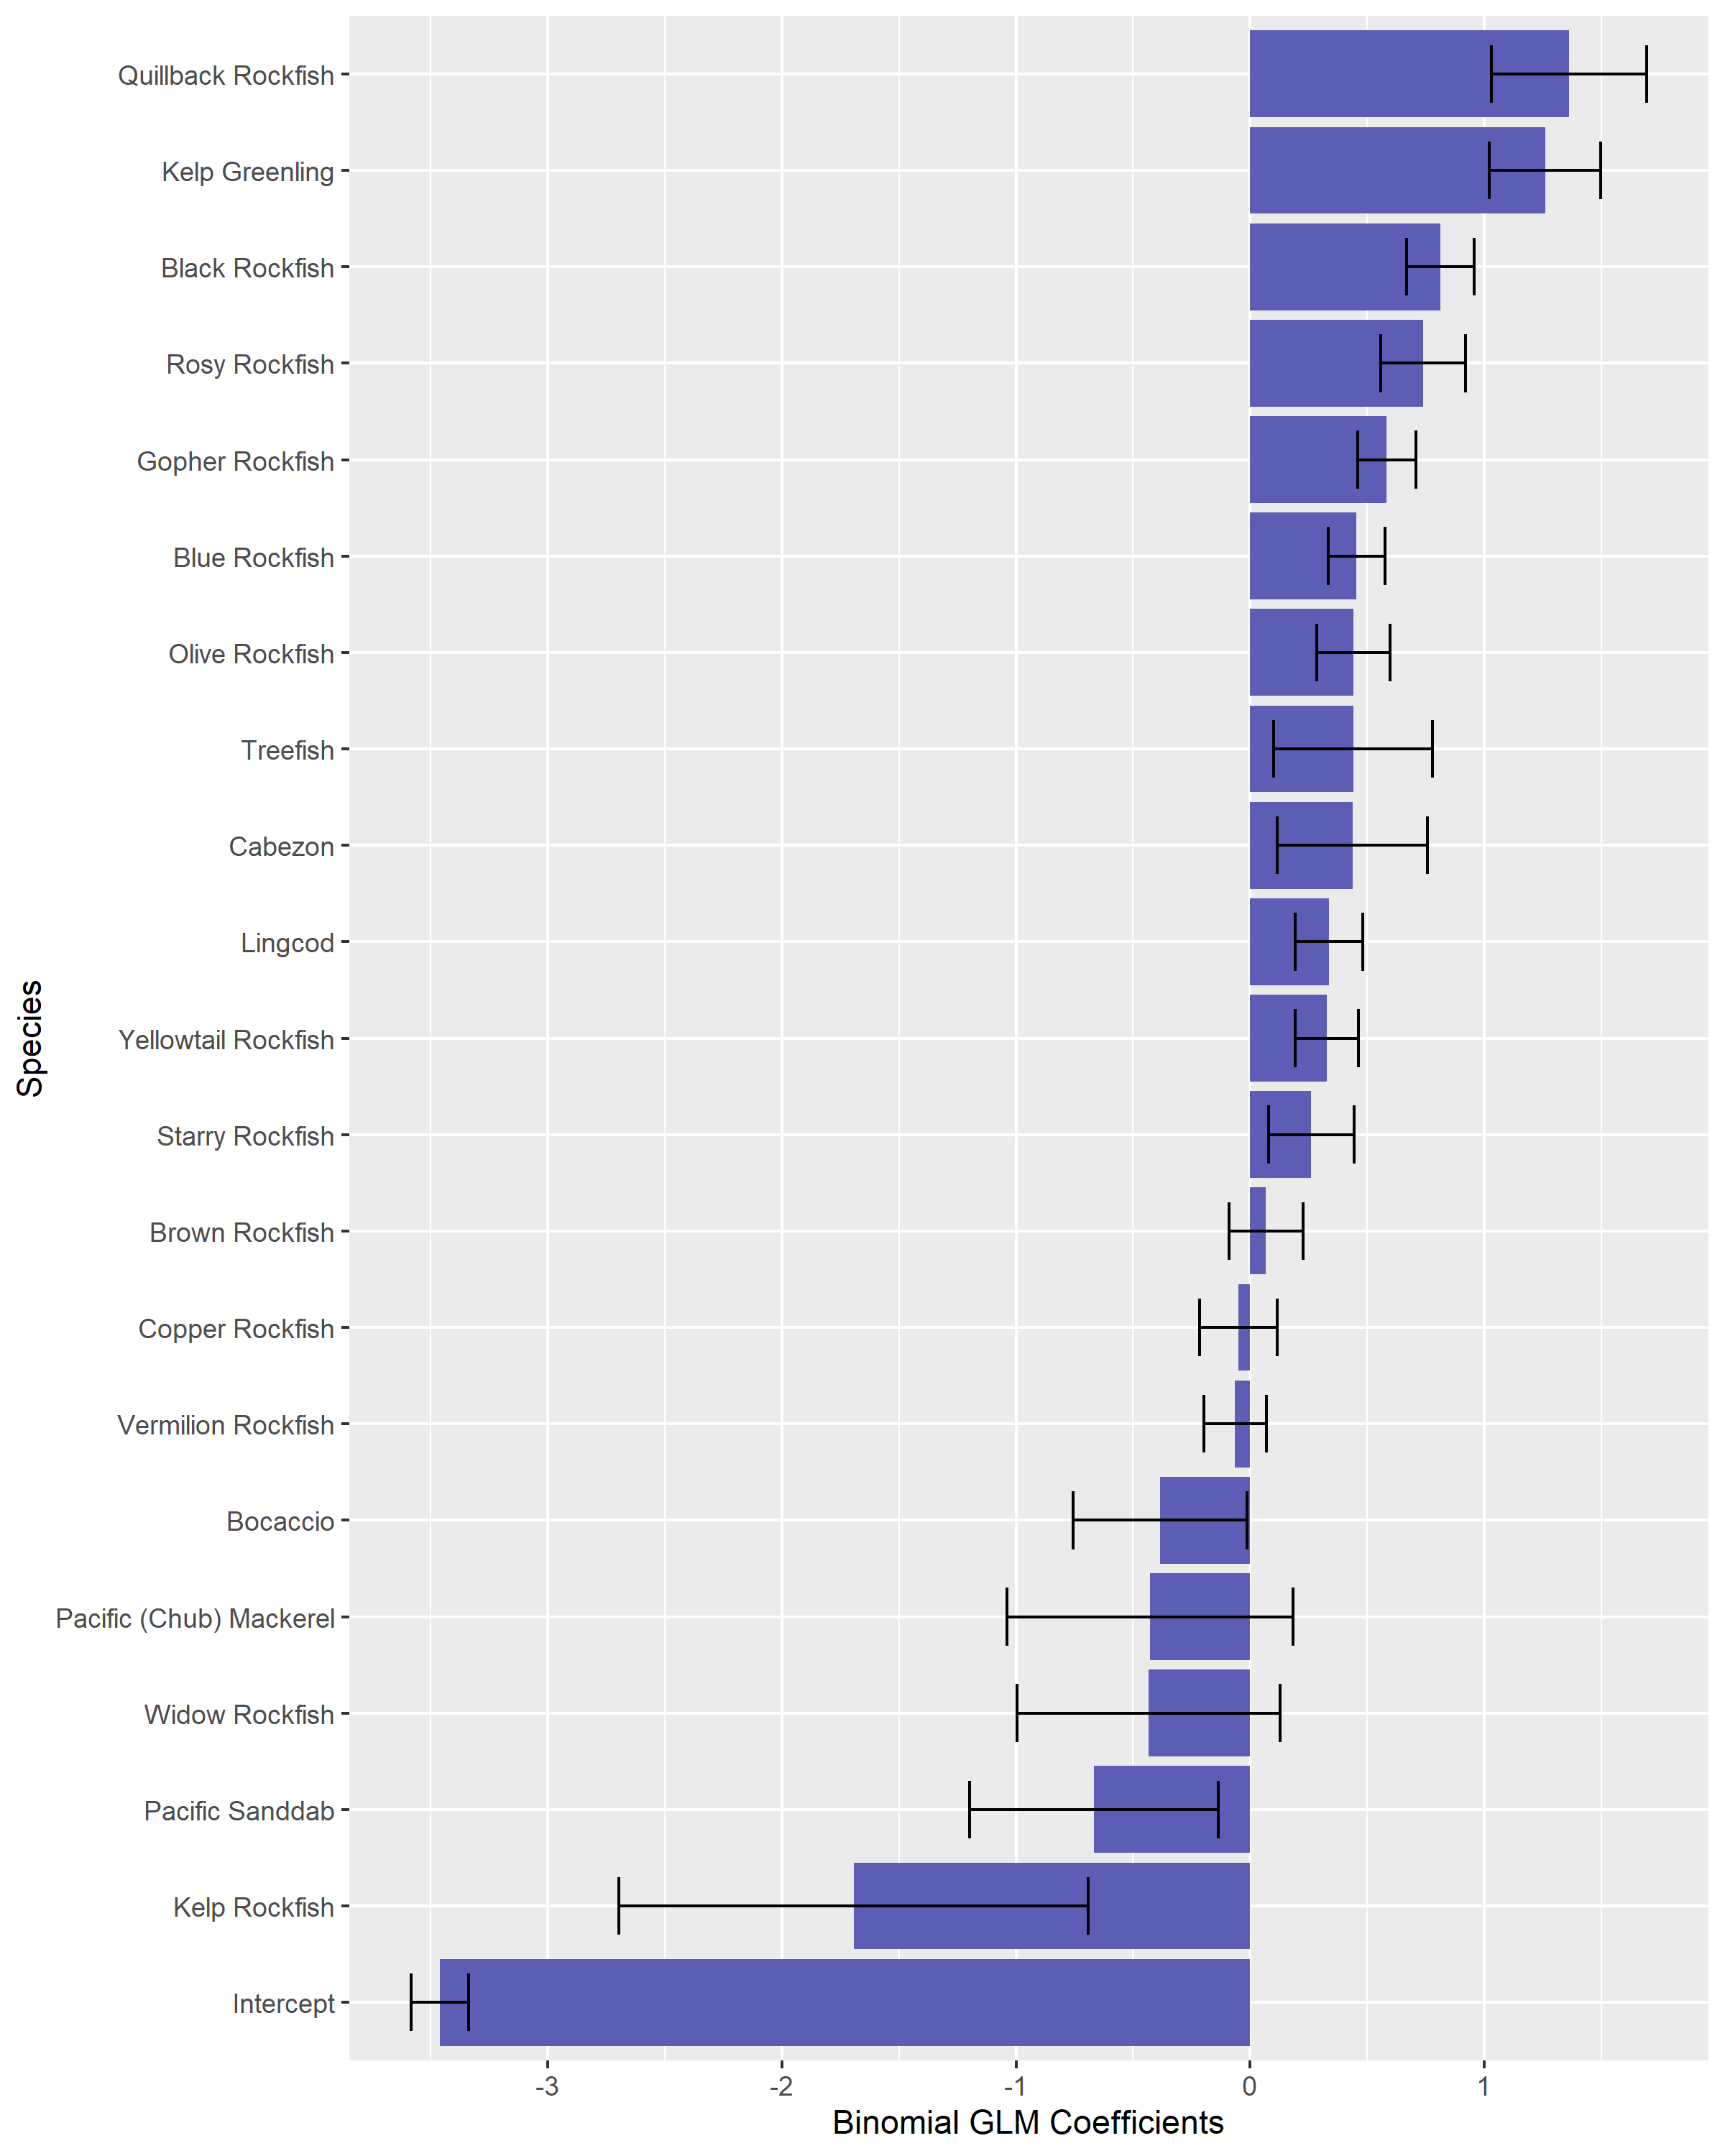
\includegraphics[width=2.75in,height=\textheight]{figures/china_drift_sm.png}

}

}

\subcaption{\label{fig-china-driftsm}China rockfish drift level}
\end{minipage}%

\caption{\label{fig-sm2}Sm figure 2}

\end{figure}

\begin{figure}

\begin{minipage}[t]{0.50\linewidth}

{\centering 

\raisebox{-\height}{

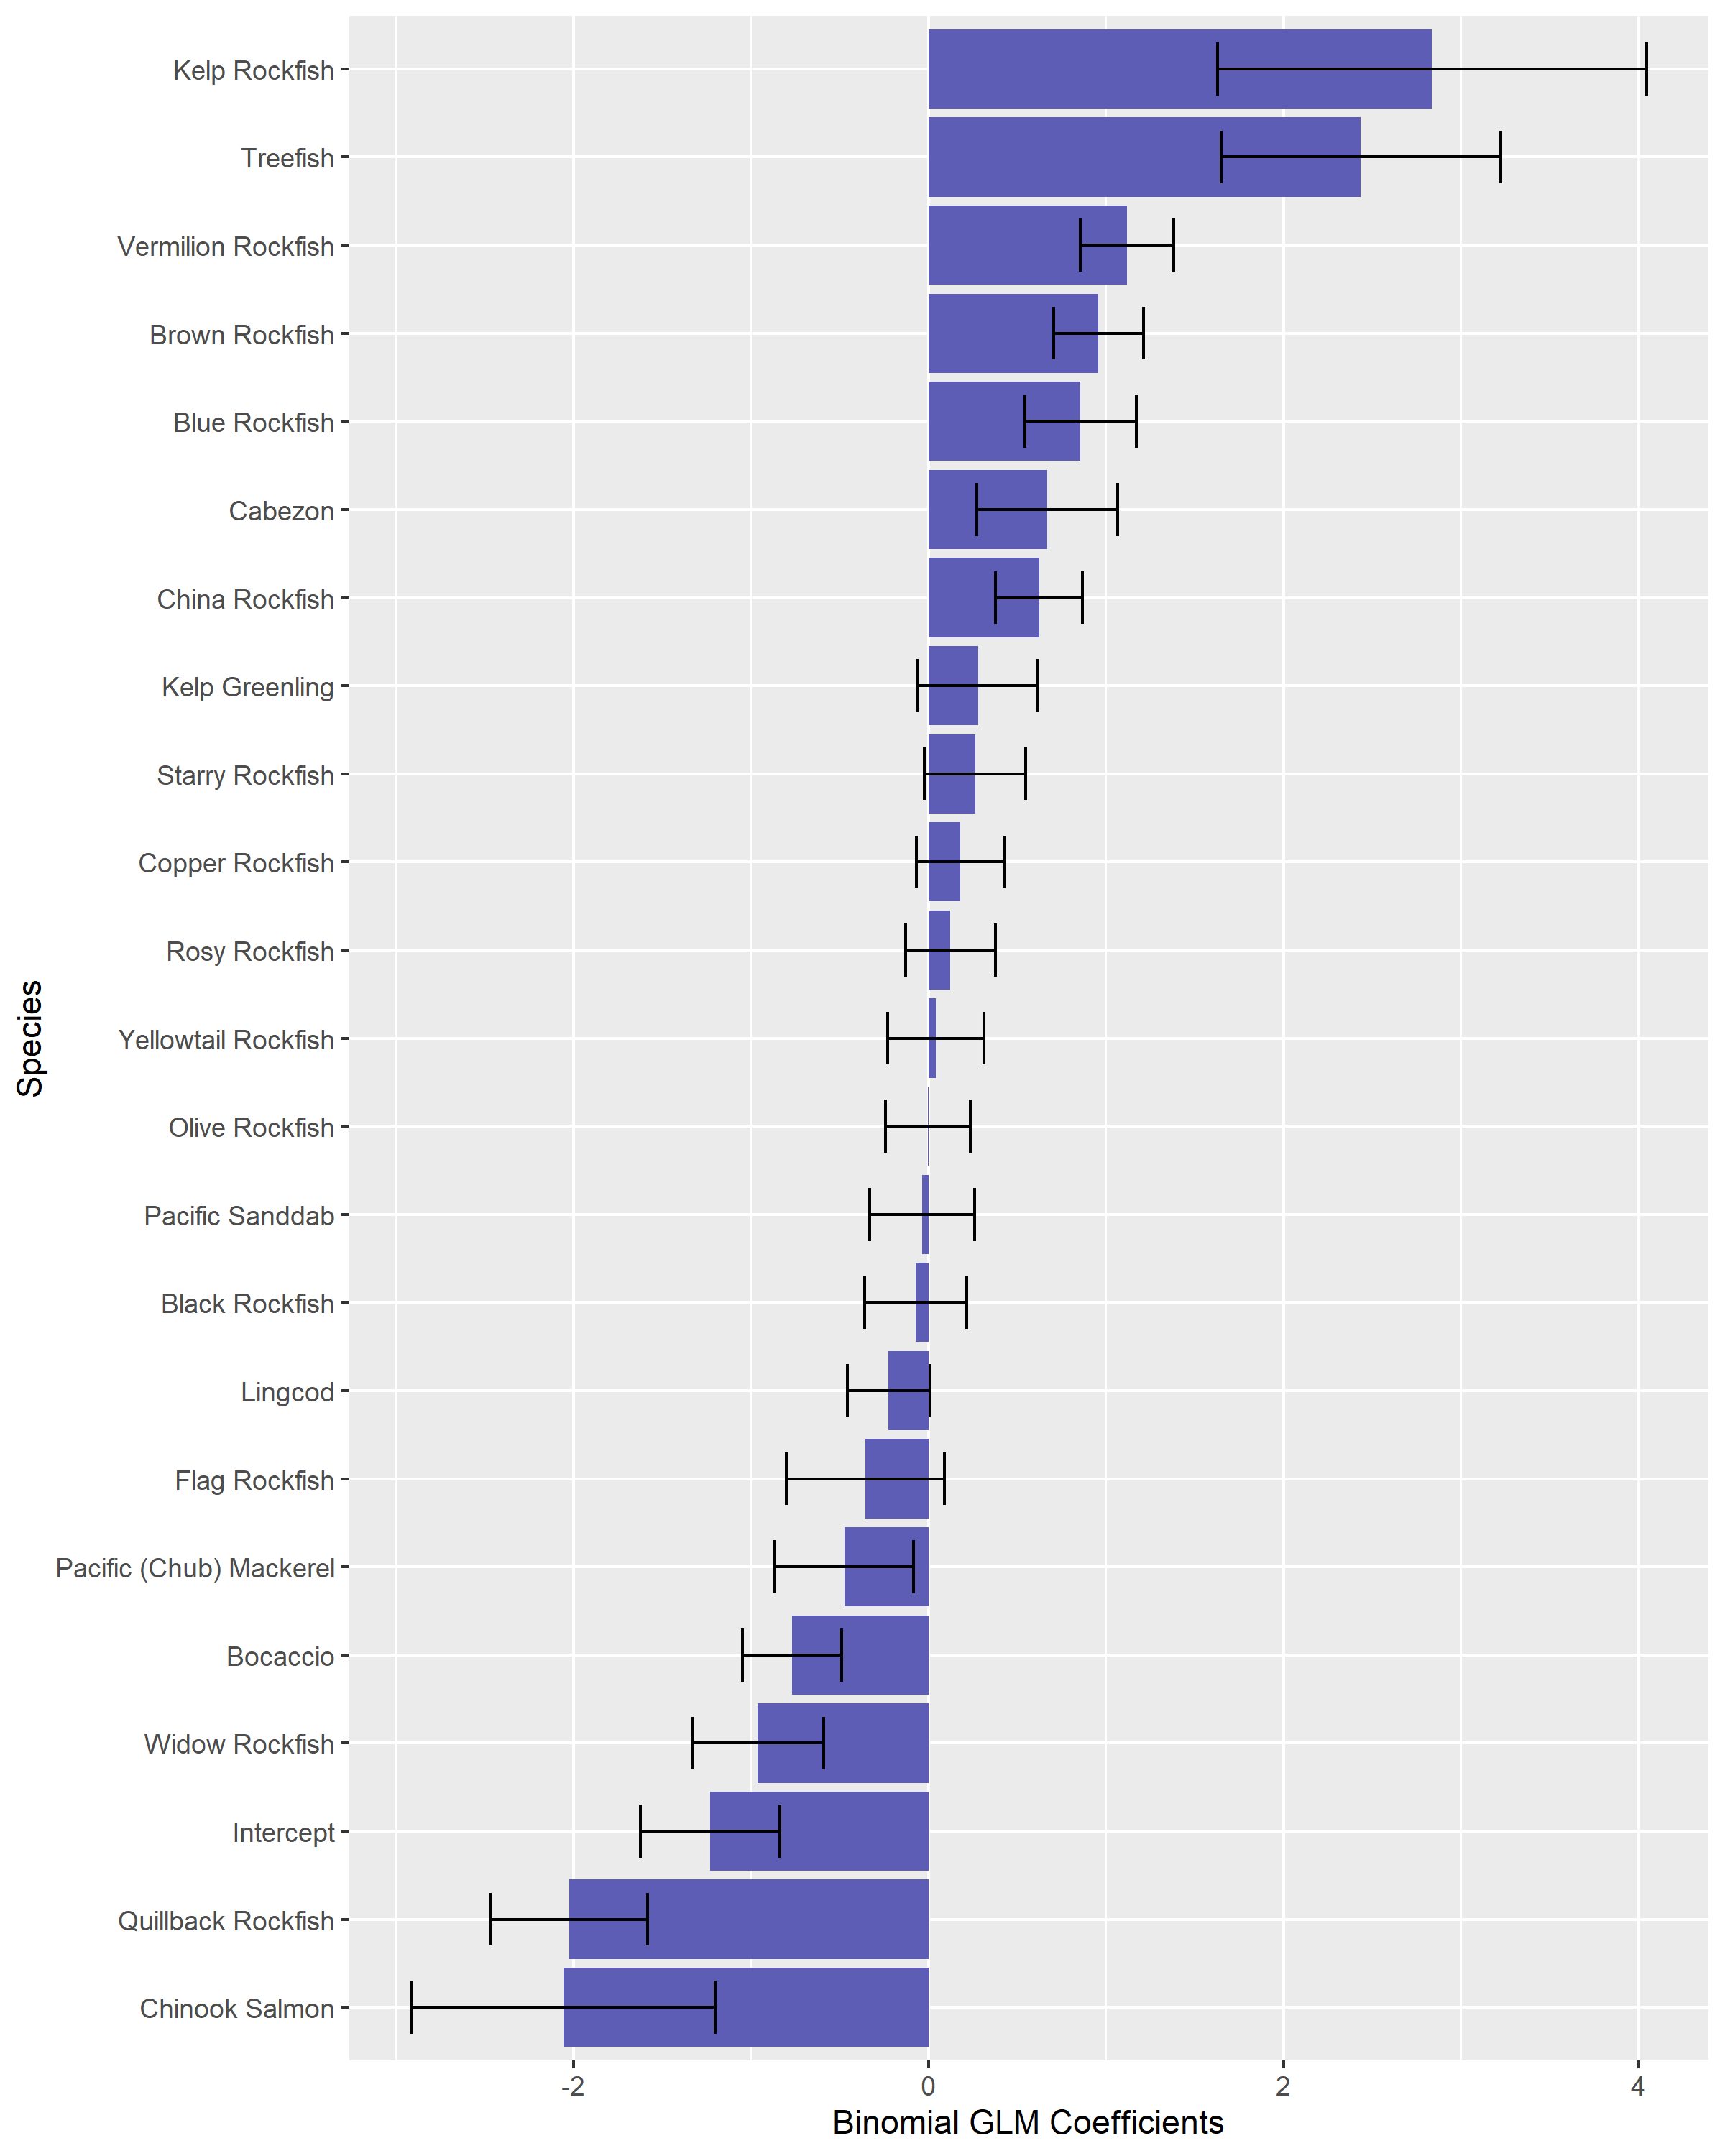
\includegraphics[width=2.75in,height=\textheight]{figures/gopher_trip_sm.png}

}

}

\subcaption{\label{fig-gopher-trips}Gopher rockfish trip level}
\end{minipage}%
%
\begin{minipage}[t]{0.50\linewidth}

{\centering 

\raisebox{-\height}{

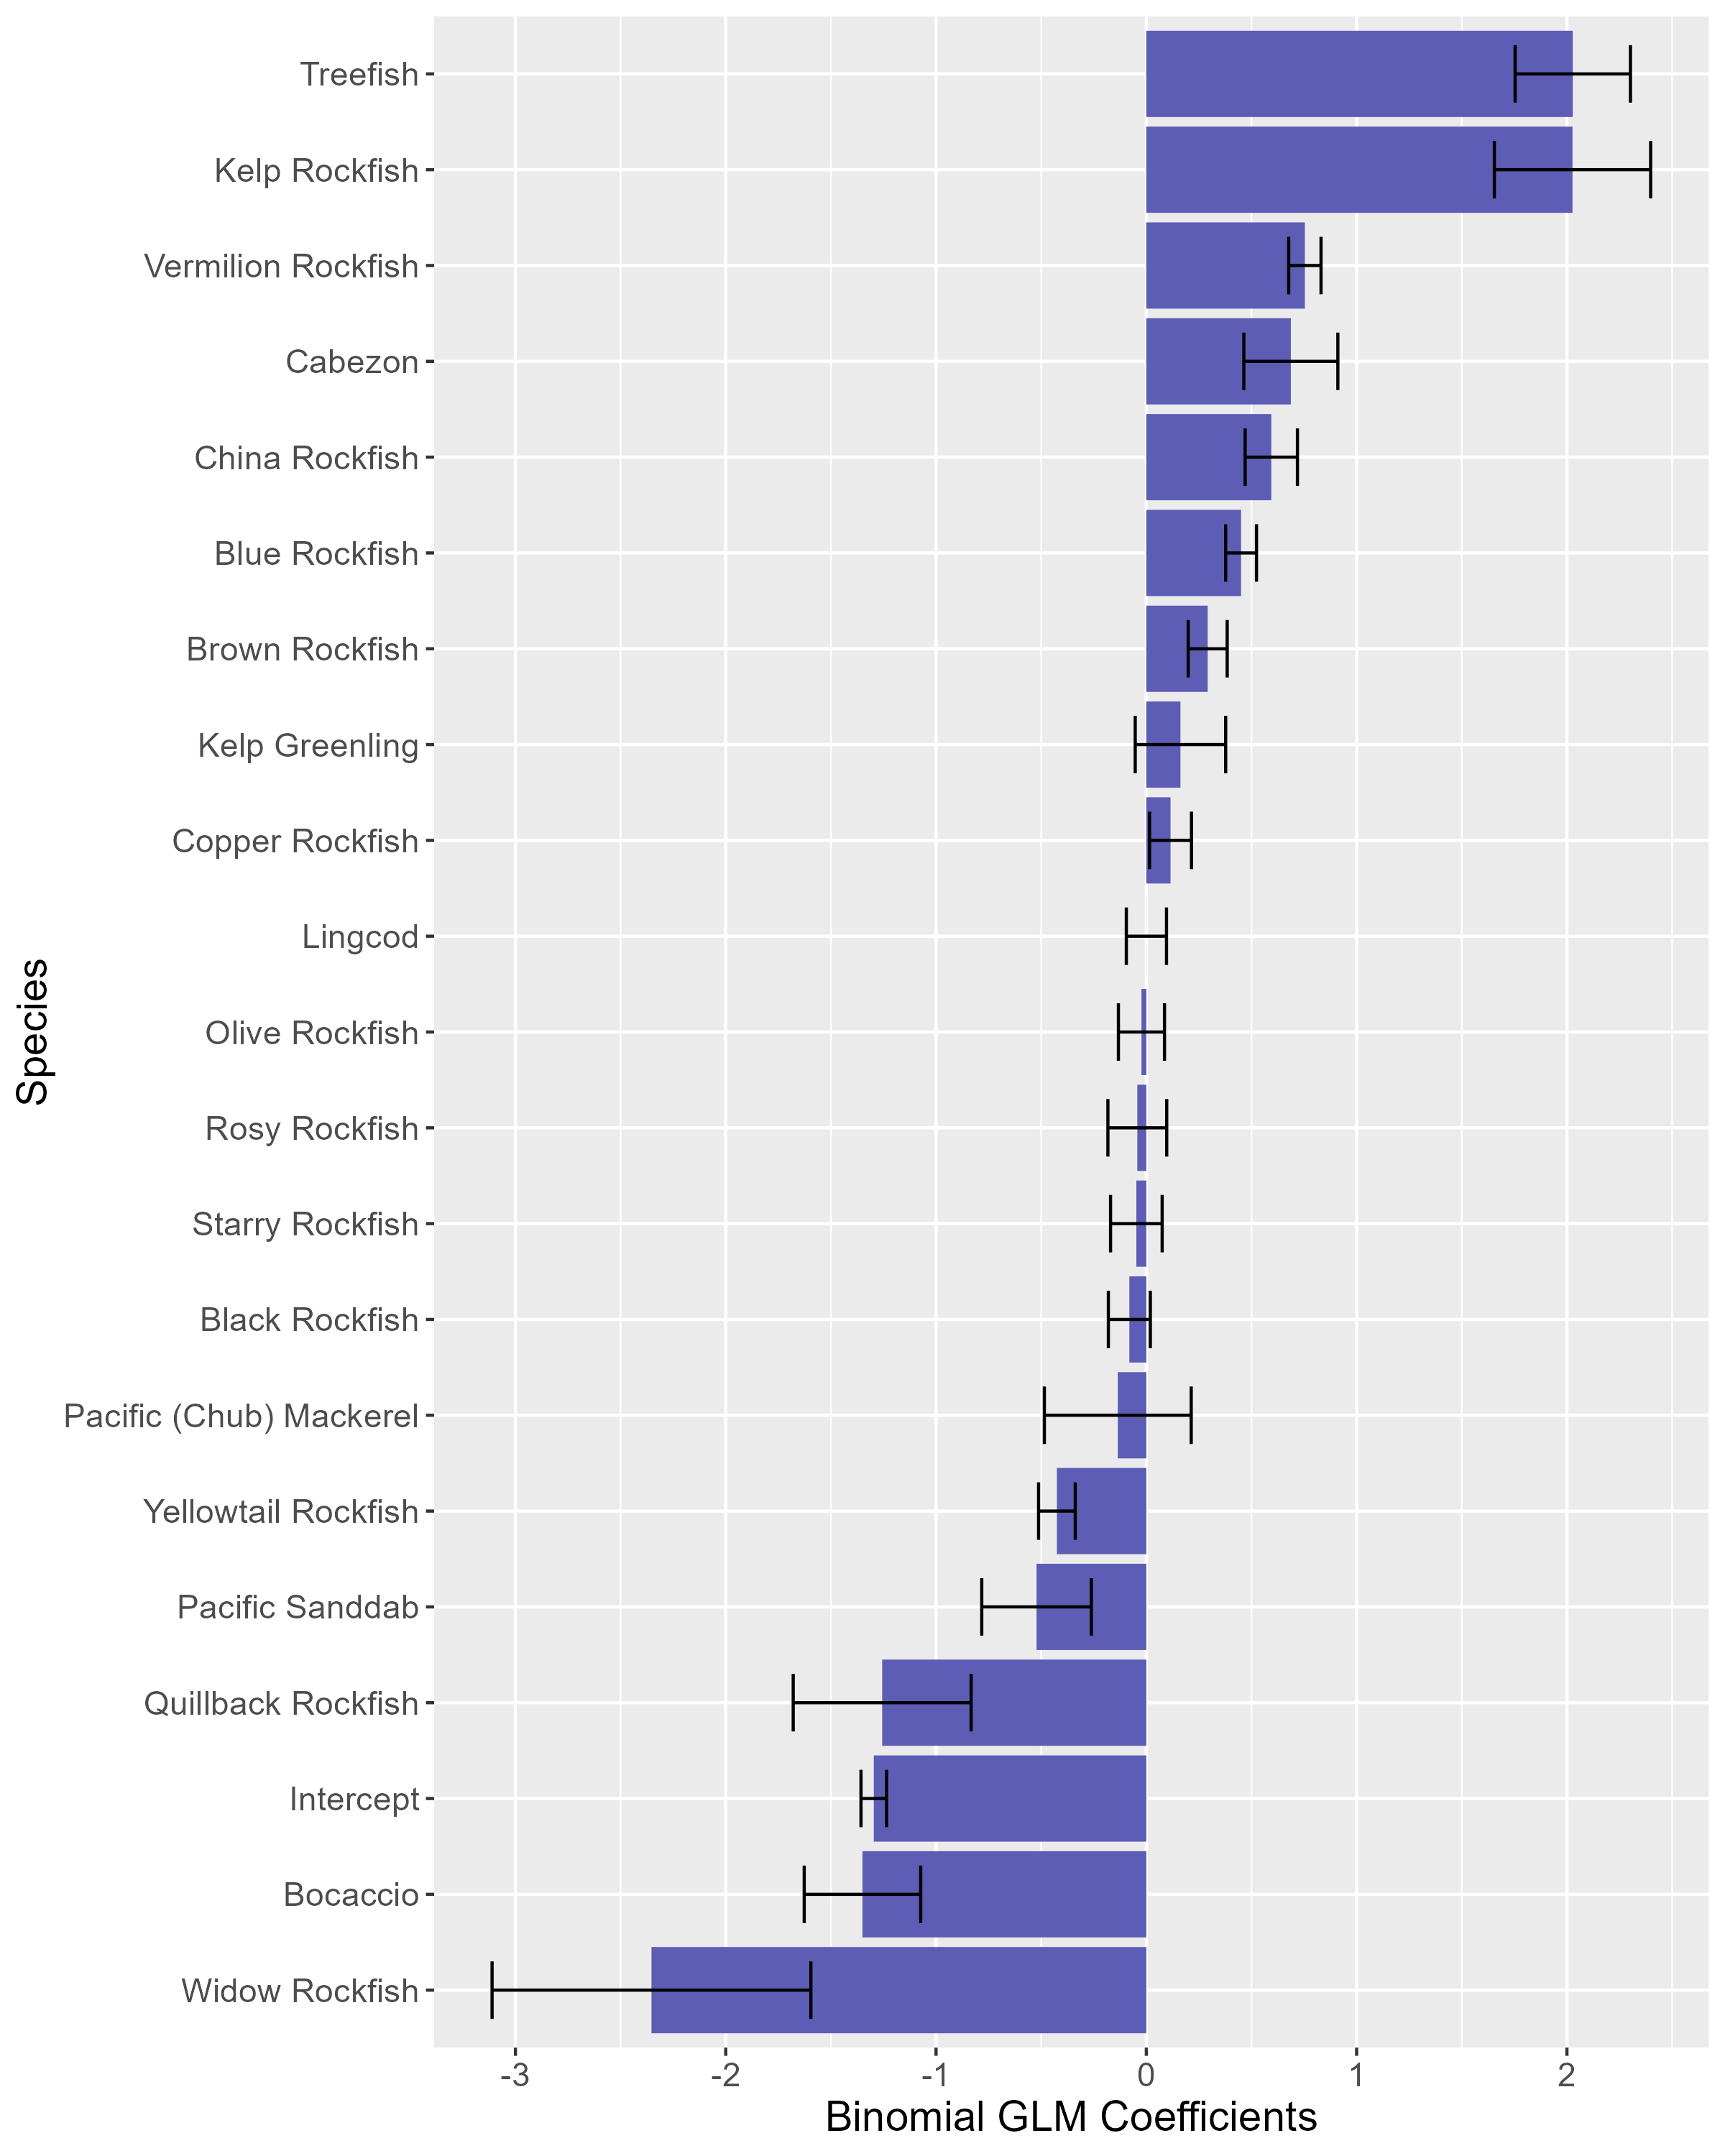
\includegraphics[width=2.75in,height=\textheight]{figures/gopher_drift_sm.png}

}

}

\subcaption{\label{fig-gopher-drifts}Gopher rockfish drift level}
\end{minipage}%
\newline
\begin{minipage}[t]{0.50\linewidth}

{\centering 

\raisebox{-\height}{

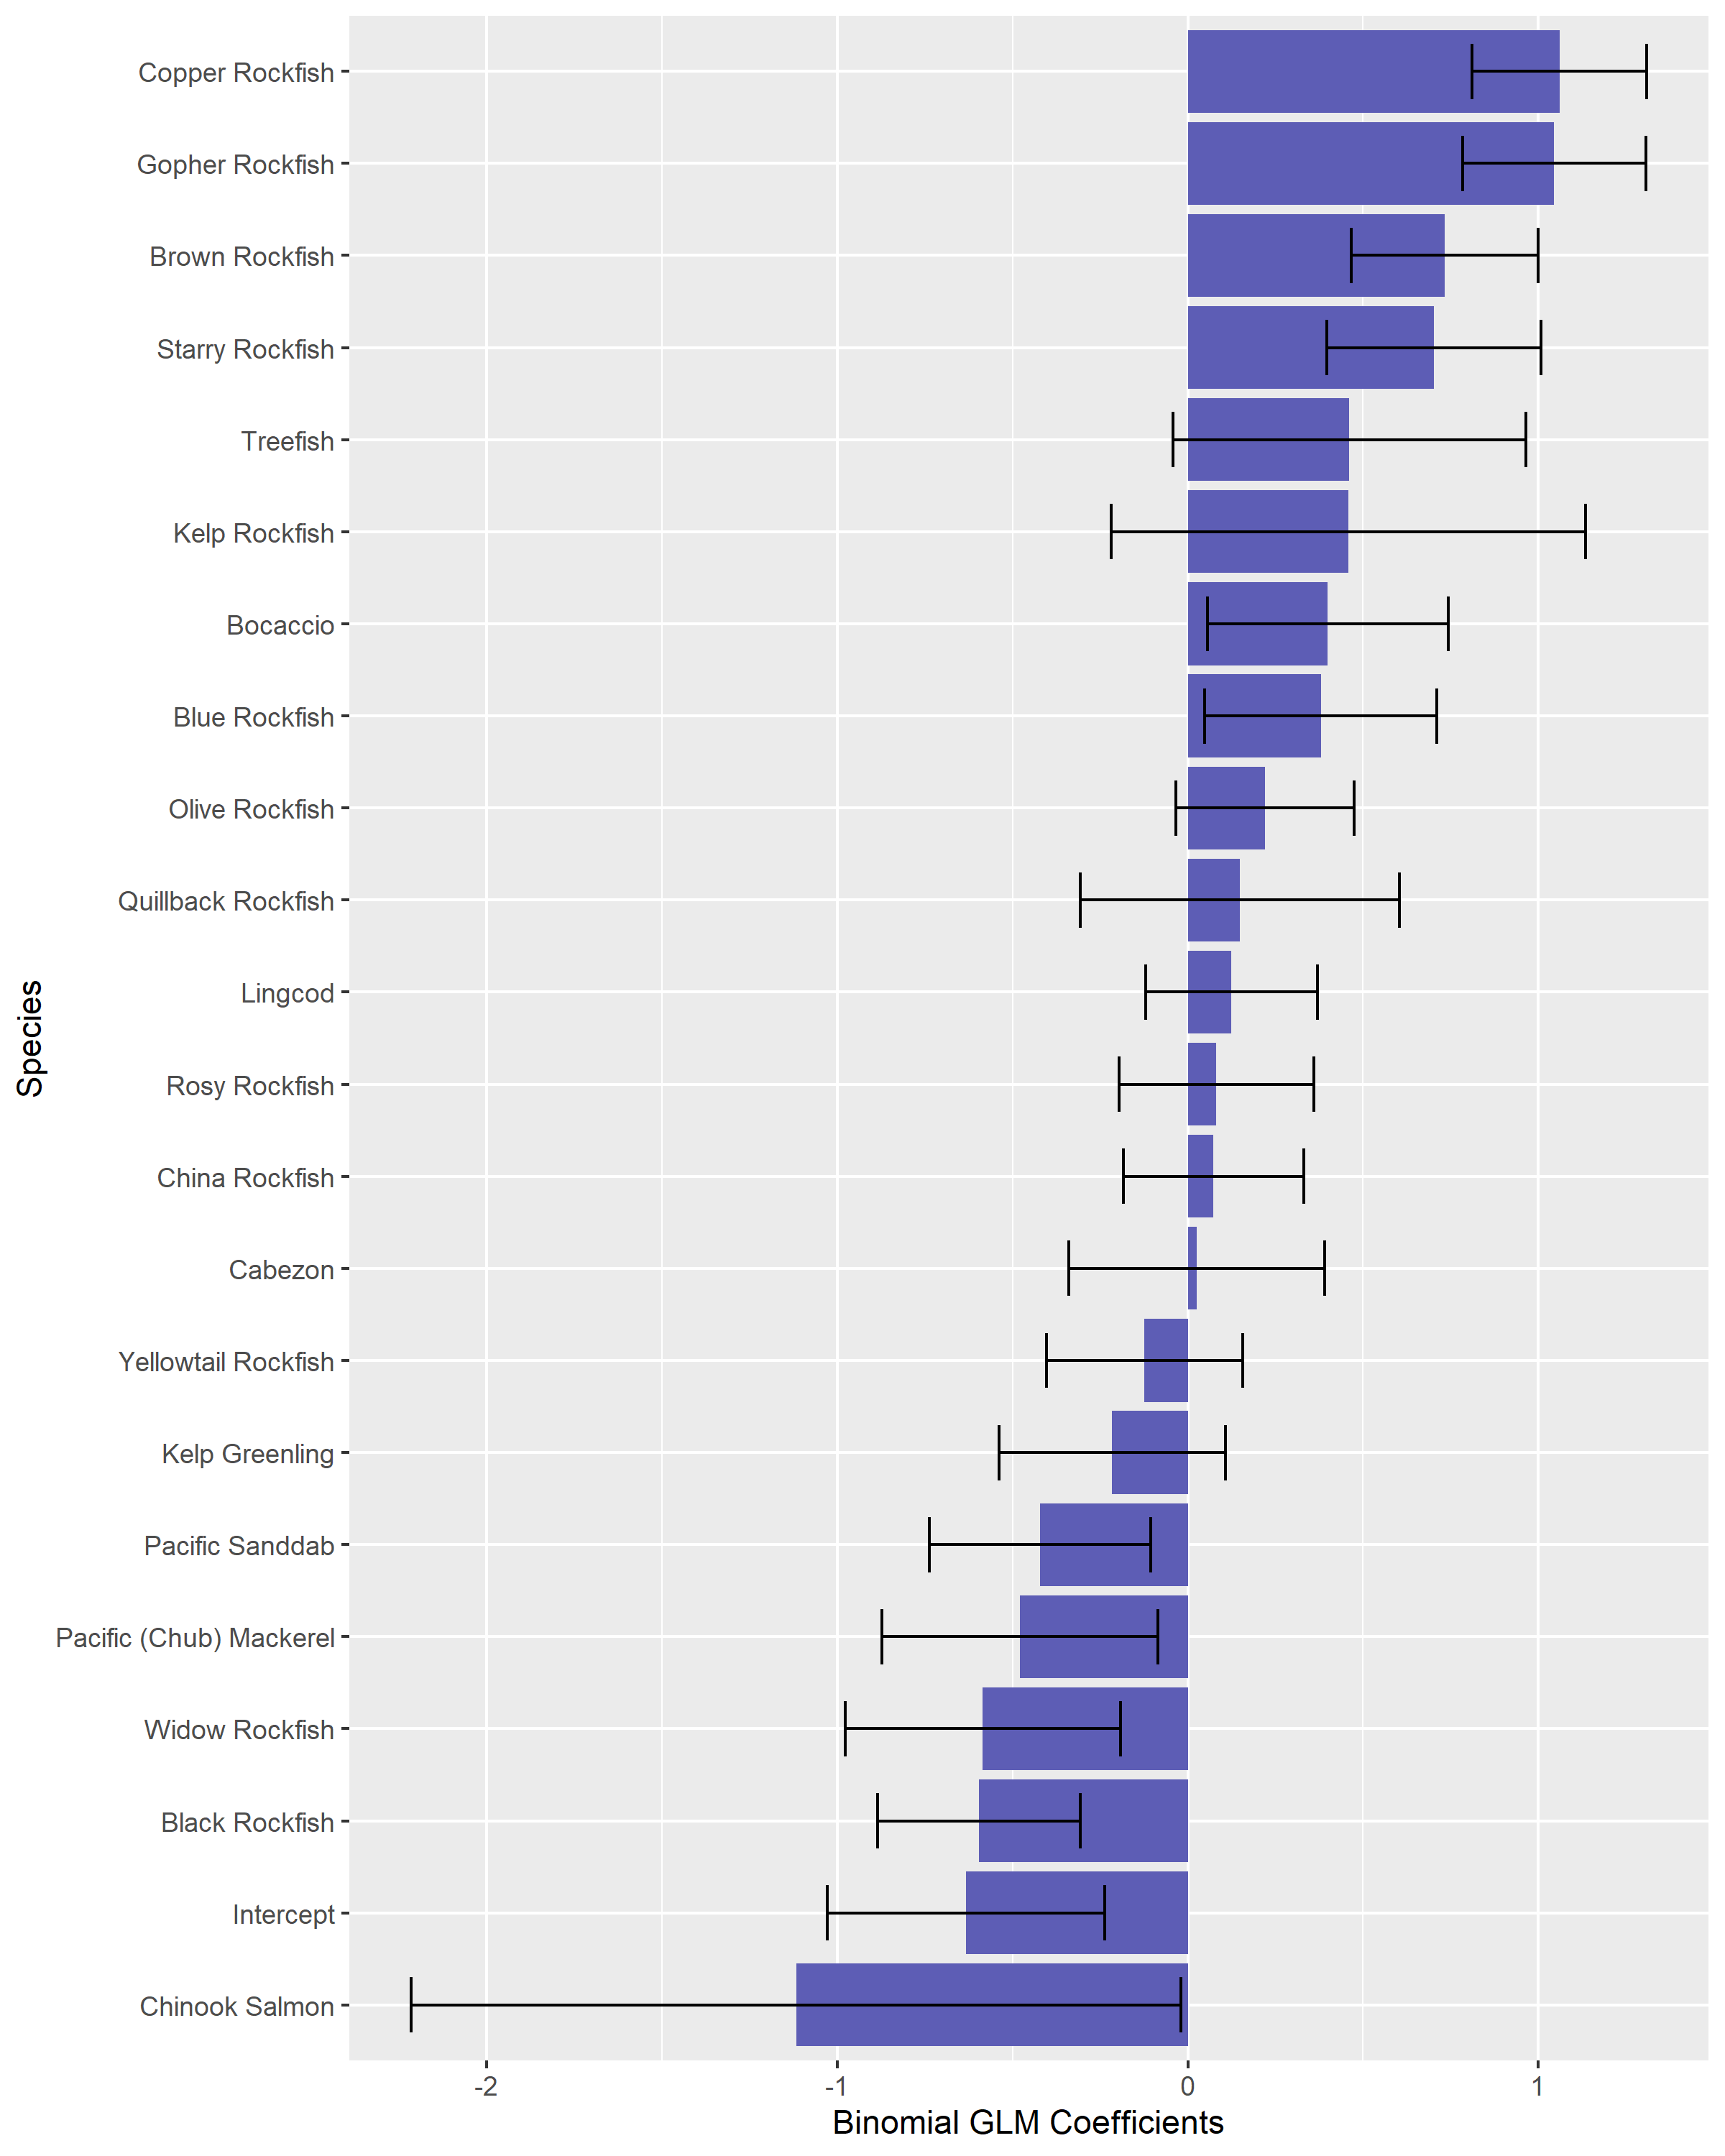
\includegraphics[width=2.75in,height=\textheight]{figures/vermilion_trip_sm.png}

}

}

\subcaption{\label{fig-vermilion-trips}Vermilion rockfish trip level}
\end{minipage}%
%
\begin{minipage}[t]{0.50\linewidth}

{\centering 

\raisebox{-\height}{

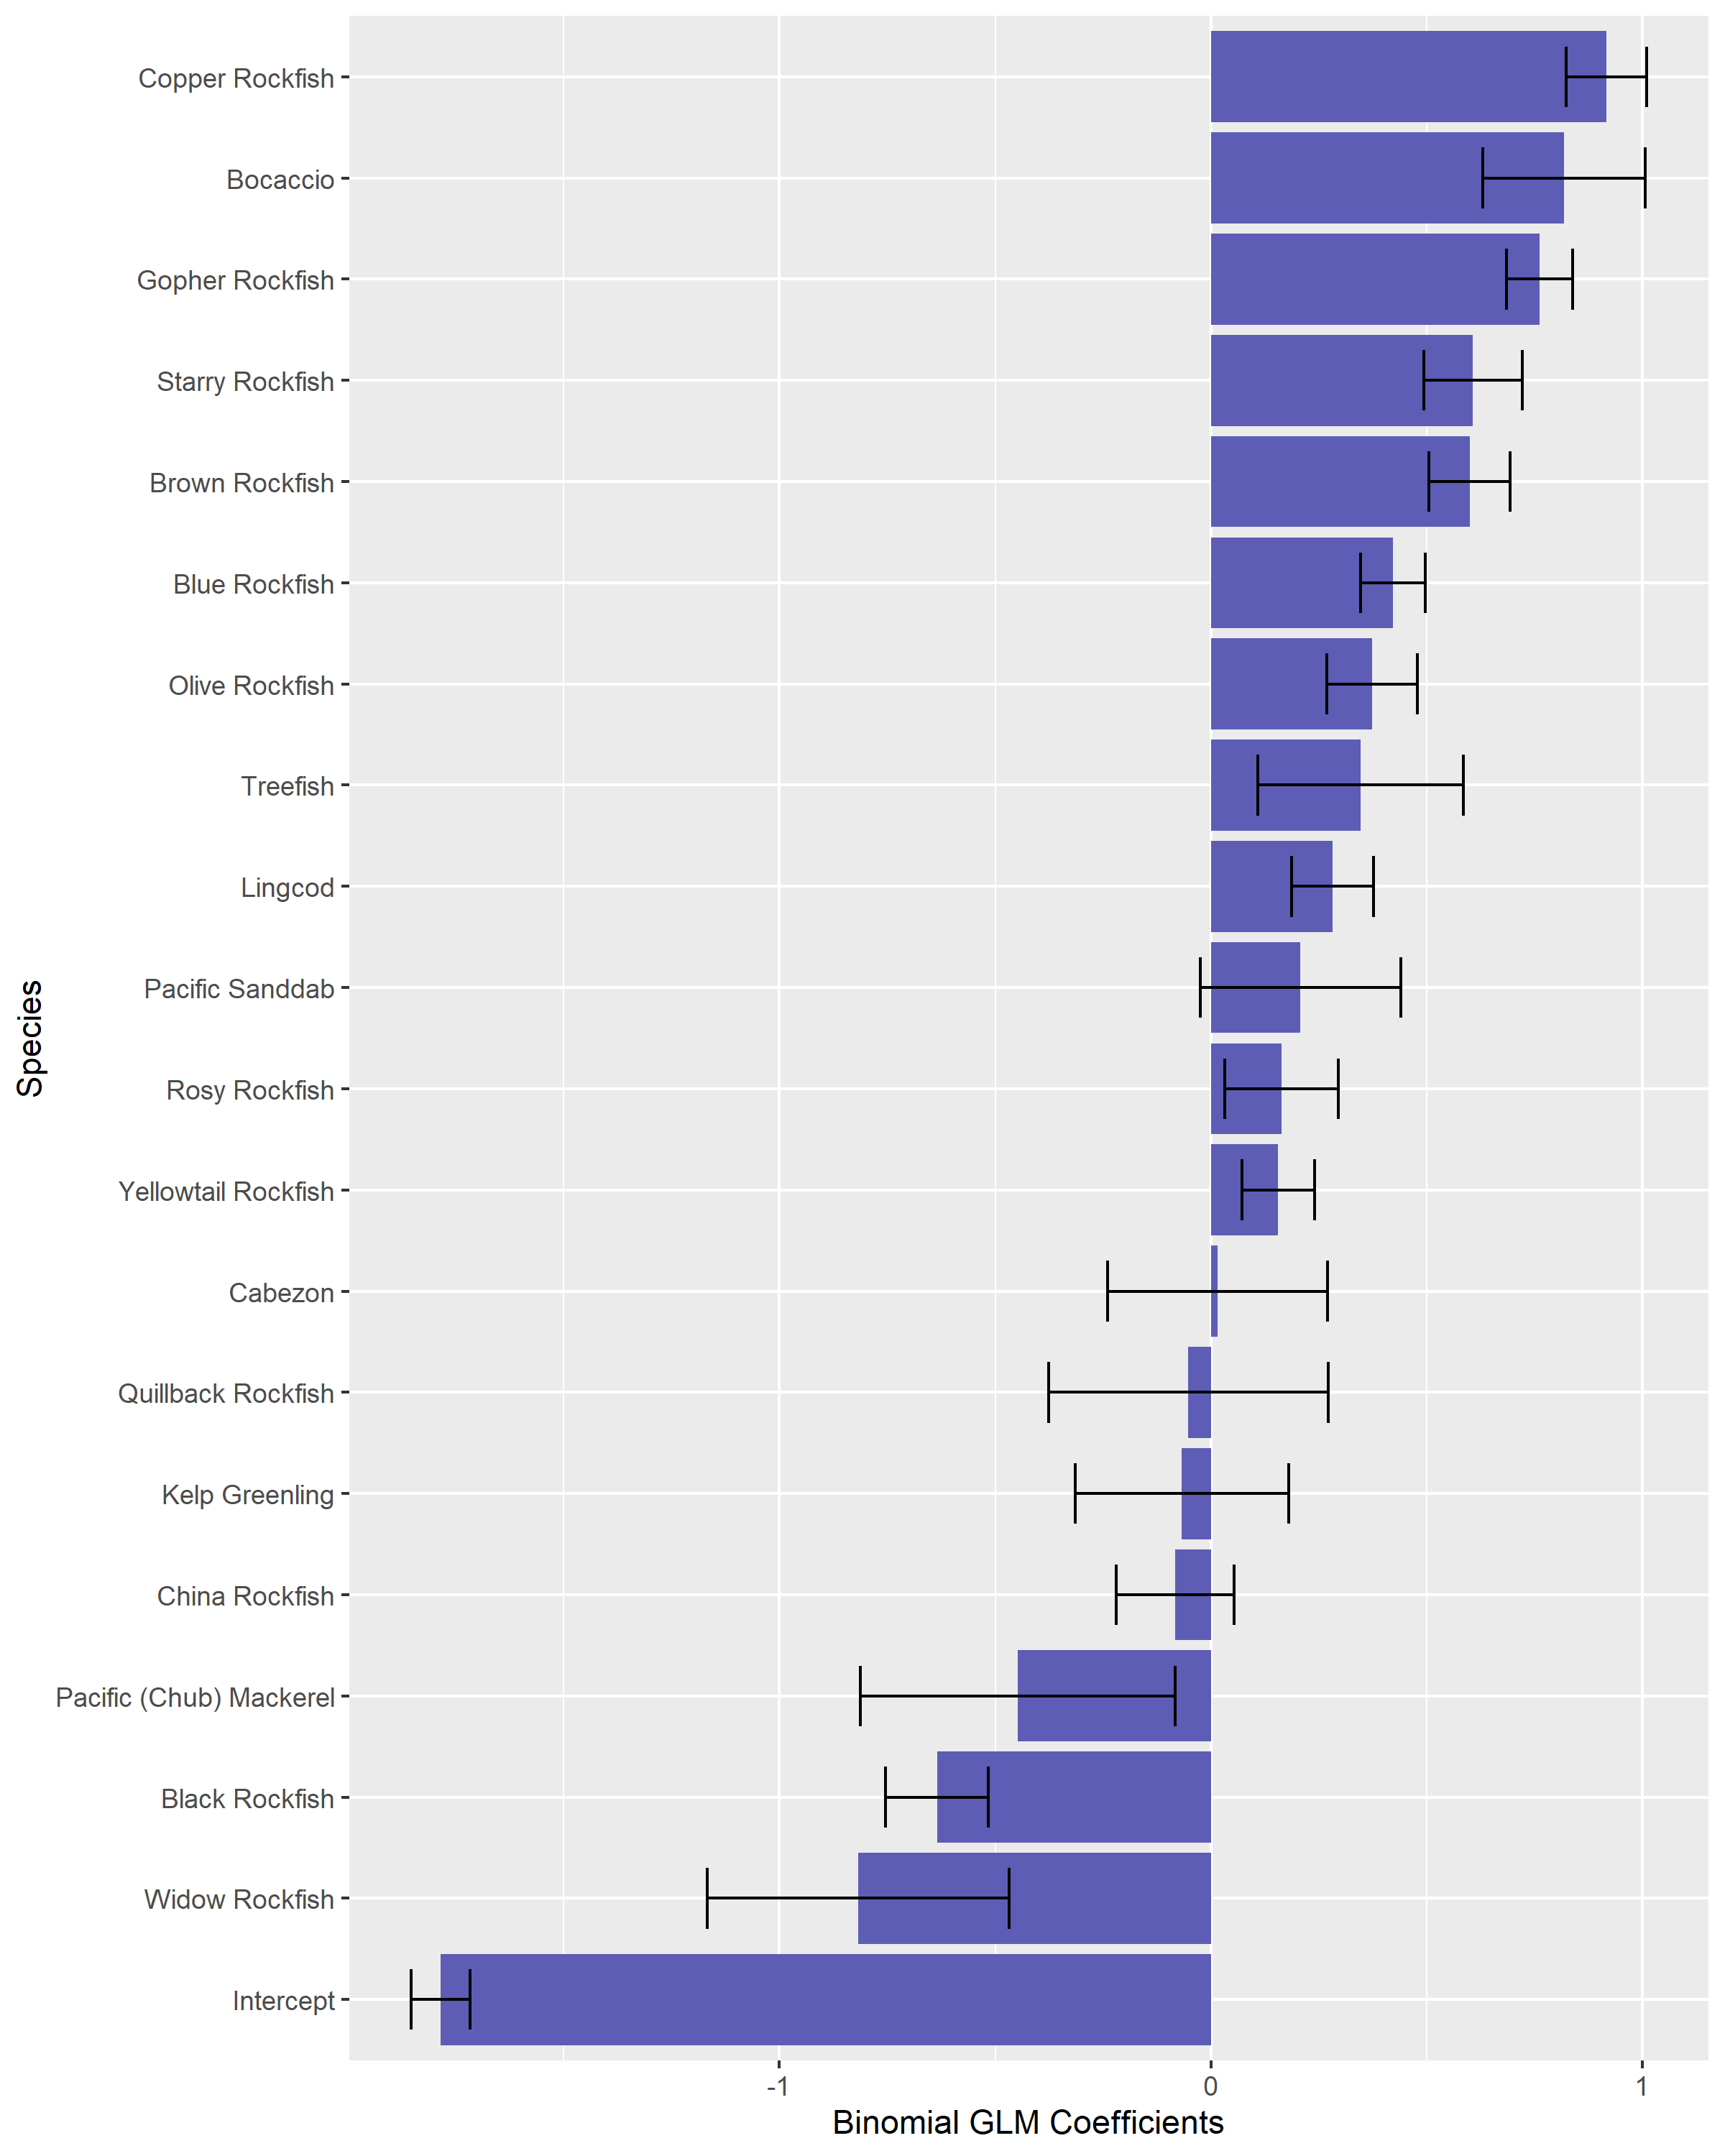
\includegraphics[width=2.75in,height=\textheight]{figures/vermilion_drift_sm.png}

}

}

\subcaption{\label{fig-vermilion-drifts}Vermilion rockfish driftlevel}
\end{minipage}%

\caption{\label{fig-sm3}SM3}

\end{figure}

\begin{figure}

\begin{minipage}[t]{0.50\linewidth}

{\centering 

\raisebox{-\height}{

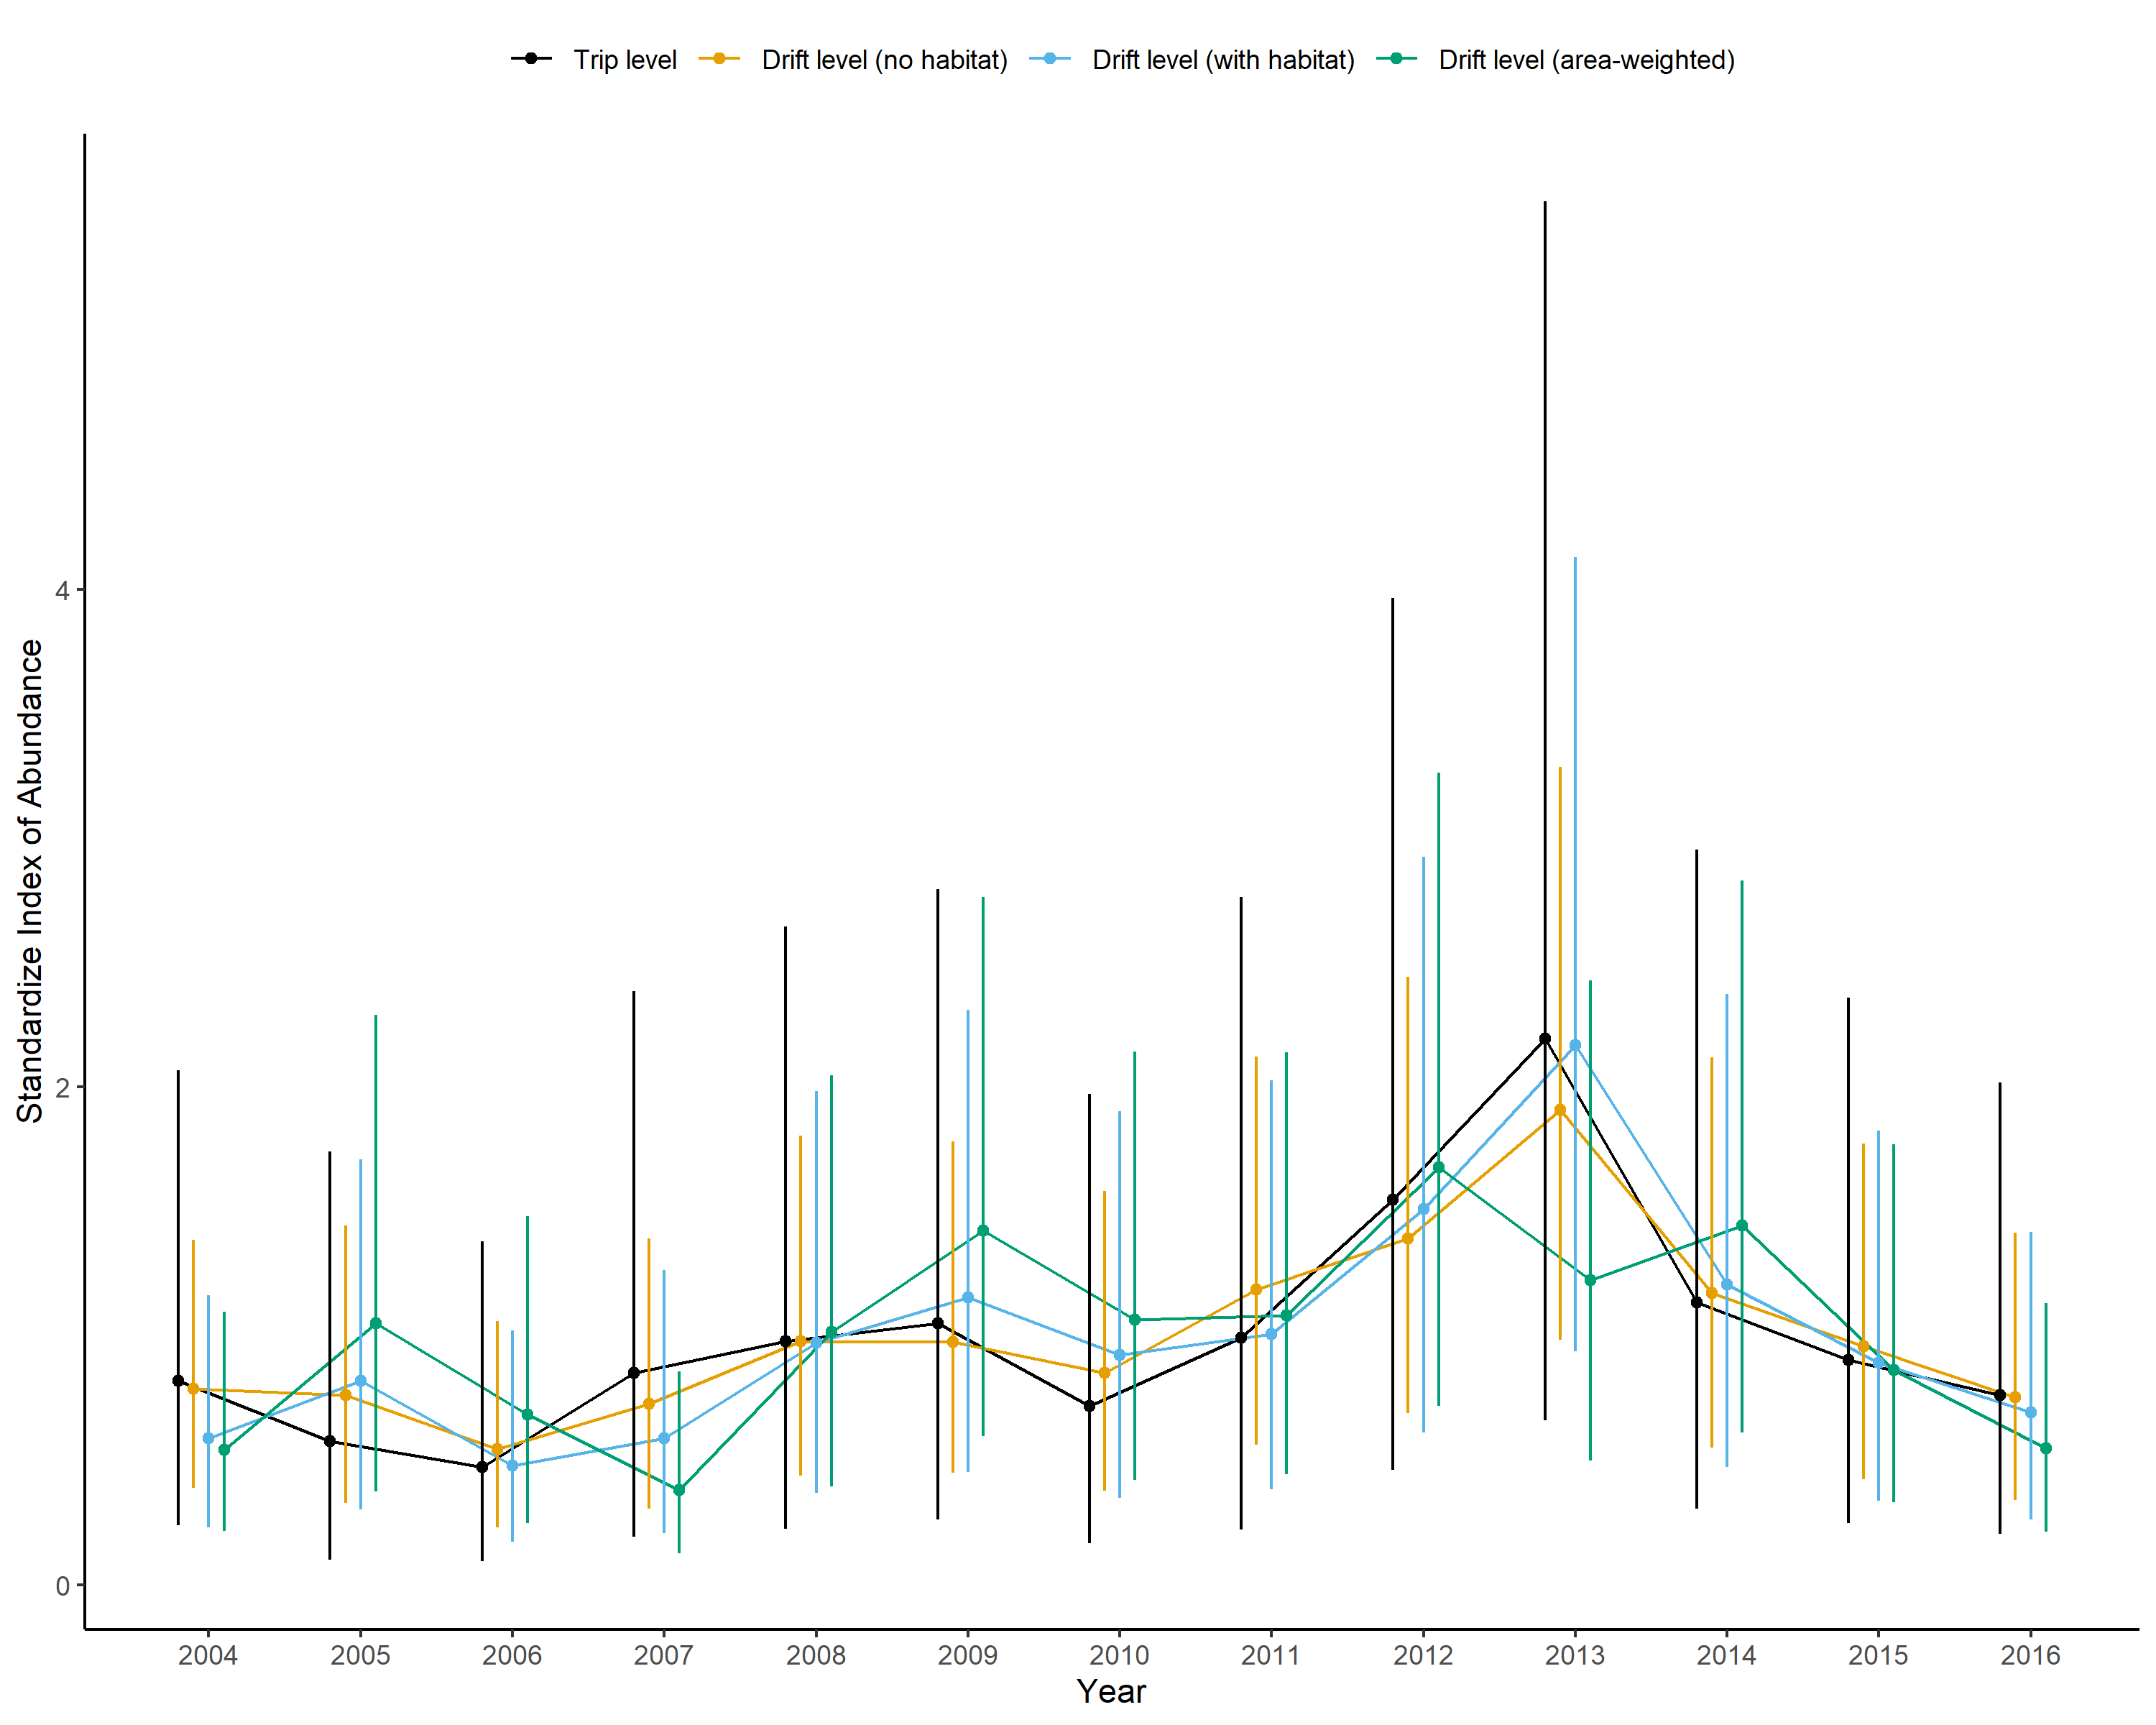
\includegraphics[width=3in,height=\textheight]{figures/black_indices.png}

}

\caption{\label{fig-black-indices}Black rockfish}

}

\end{minipage}%
%
\begin{minipage}[t]{0.50\linewidth}

{\centering 

\raisebox{-\height}{

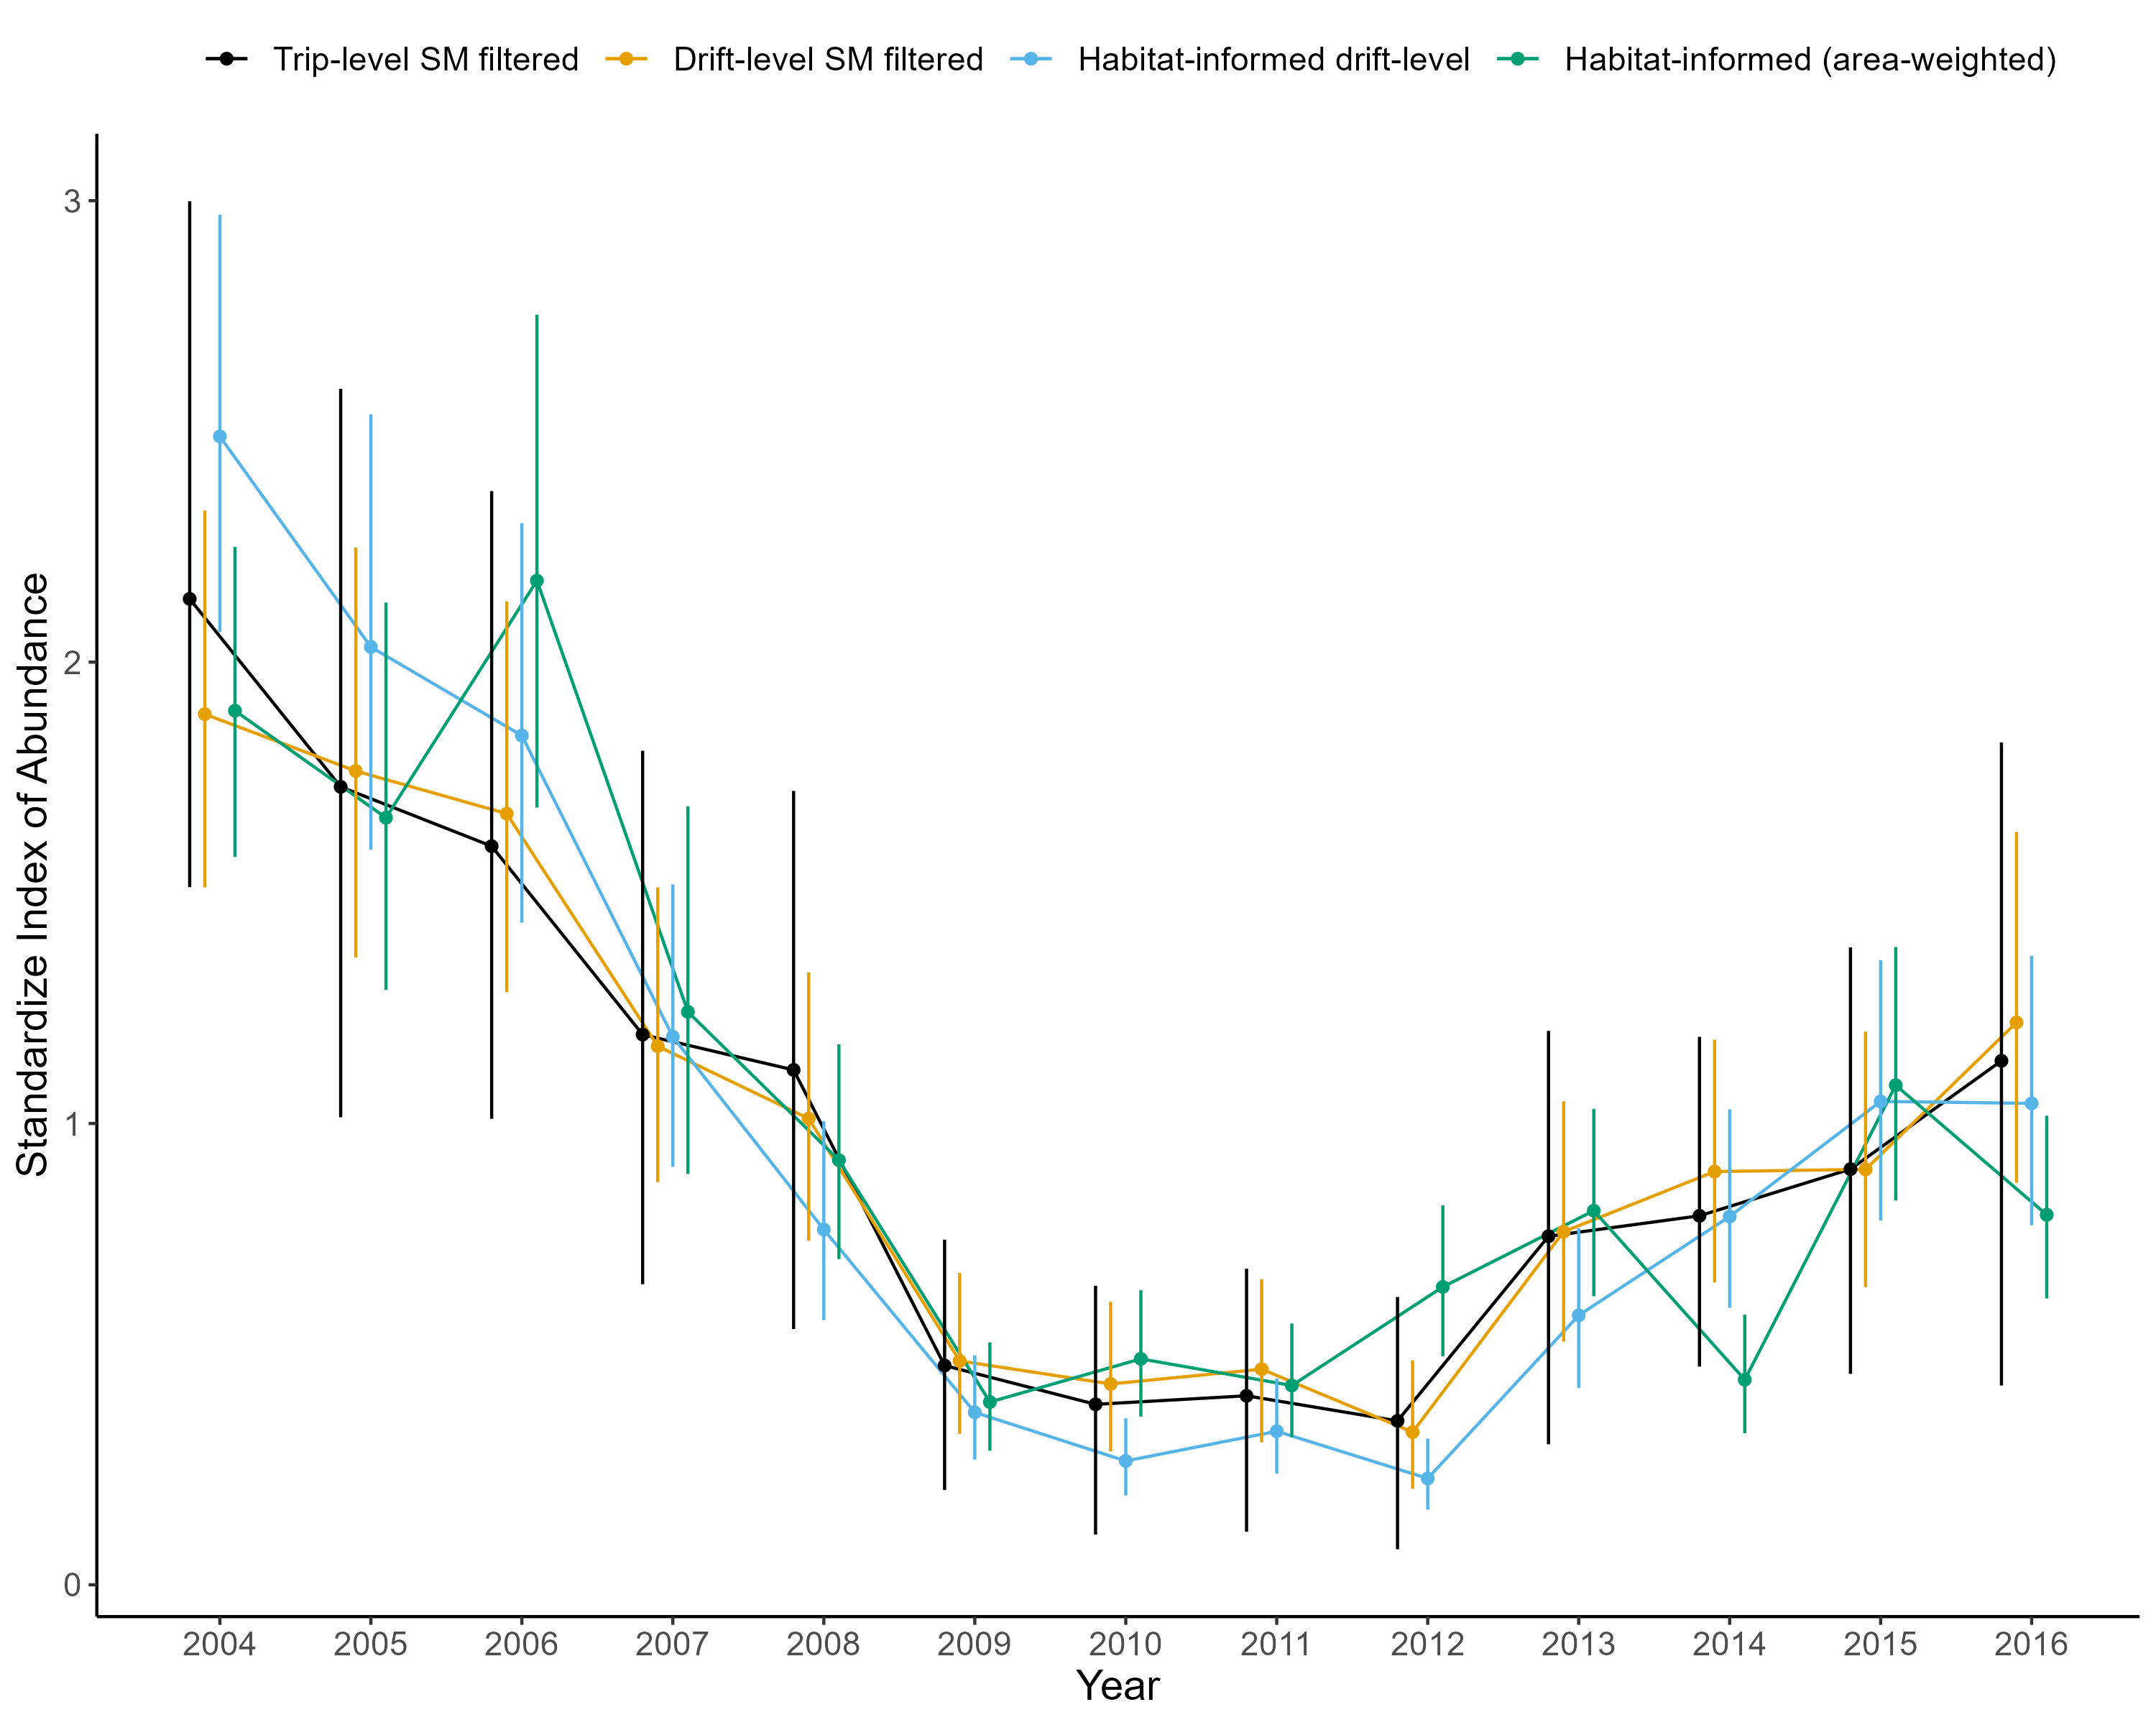
\includegraphics[width=3in,height=\textheight]{figures/blue_indices.png}

}

\caption{\label{fig-blue-indices}Blue rockfish}

}

\end{minipage}%
\newline
\begin{minipage}[t]{0.50\linewidth}

{\centering 

\raisebox{-\height}{

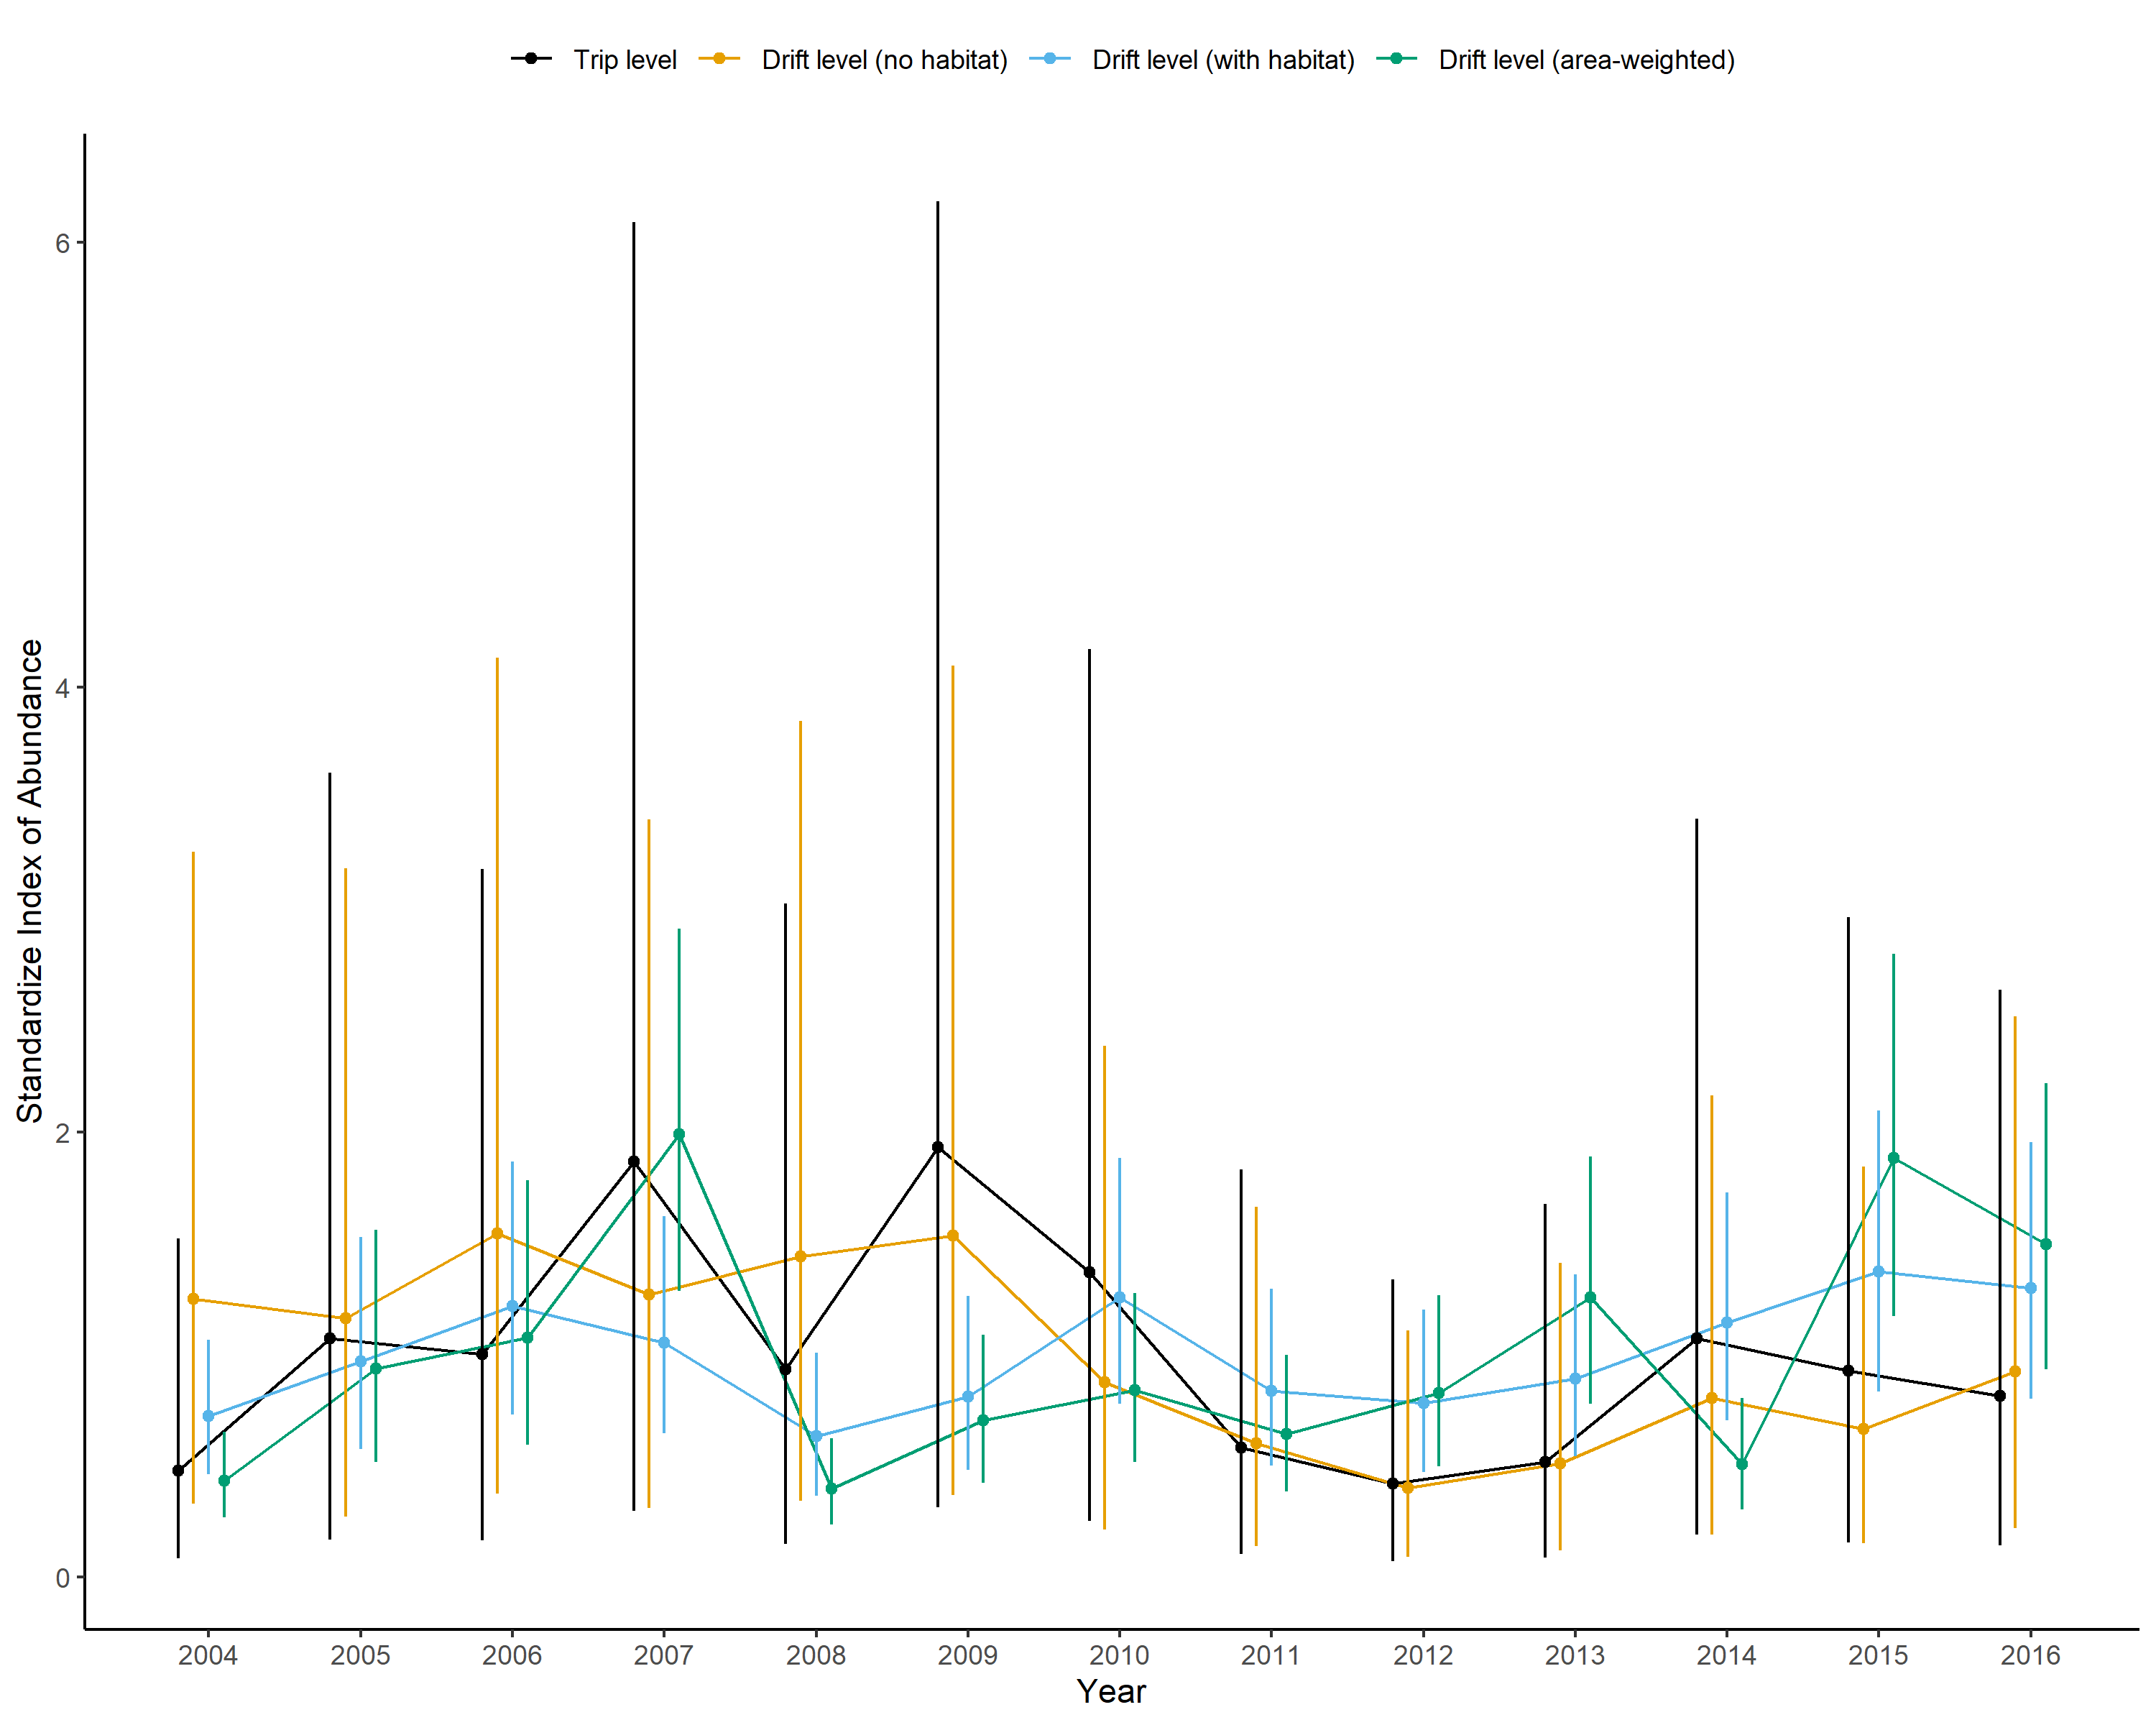
\includegraphics[width=3in,height=\textheight]{figures/brown_indices.png}

}

\caption{\label{fig-brown-indices}Brown rockfish}

}

\end{minipage}%
%
\begin{minipage}[t]{0.50\linewidth}

{\centering 

\raisebox{-\height}{

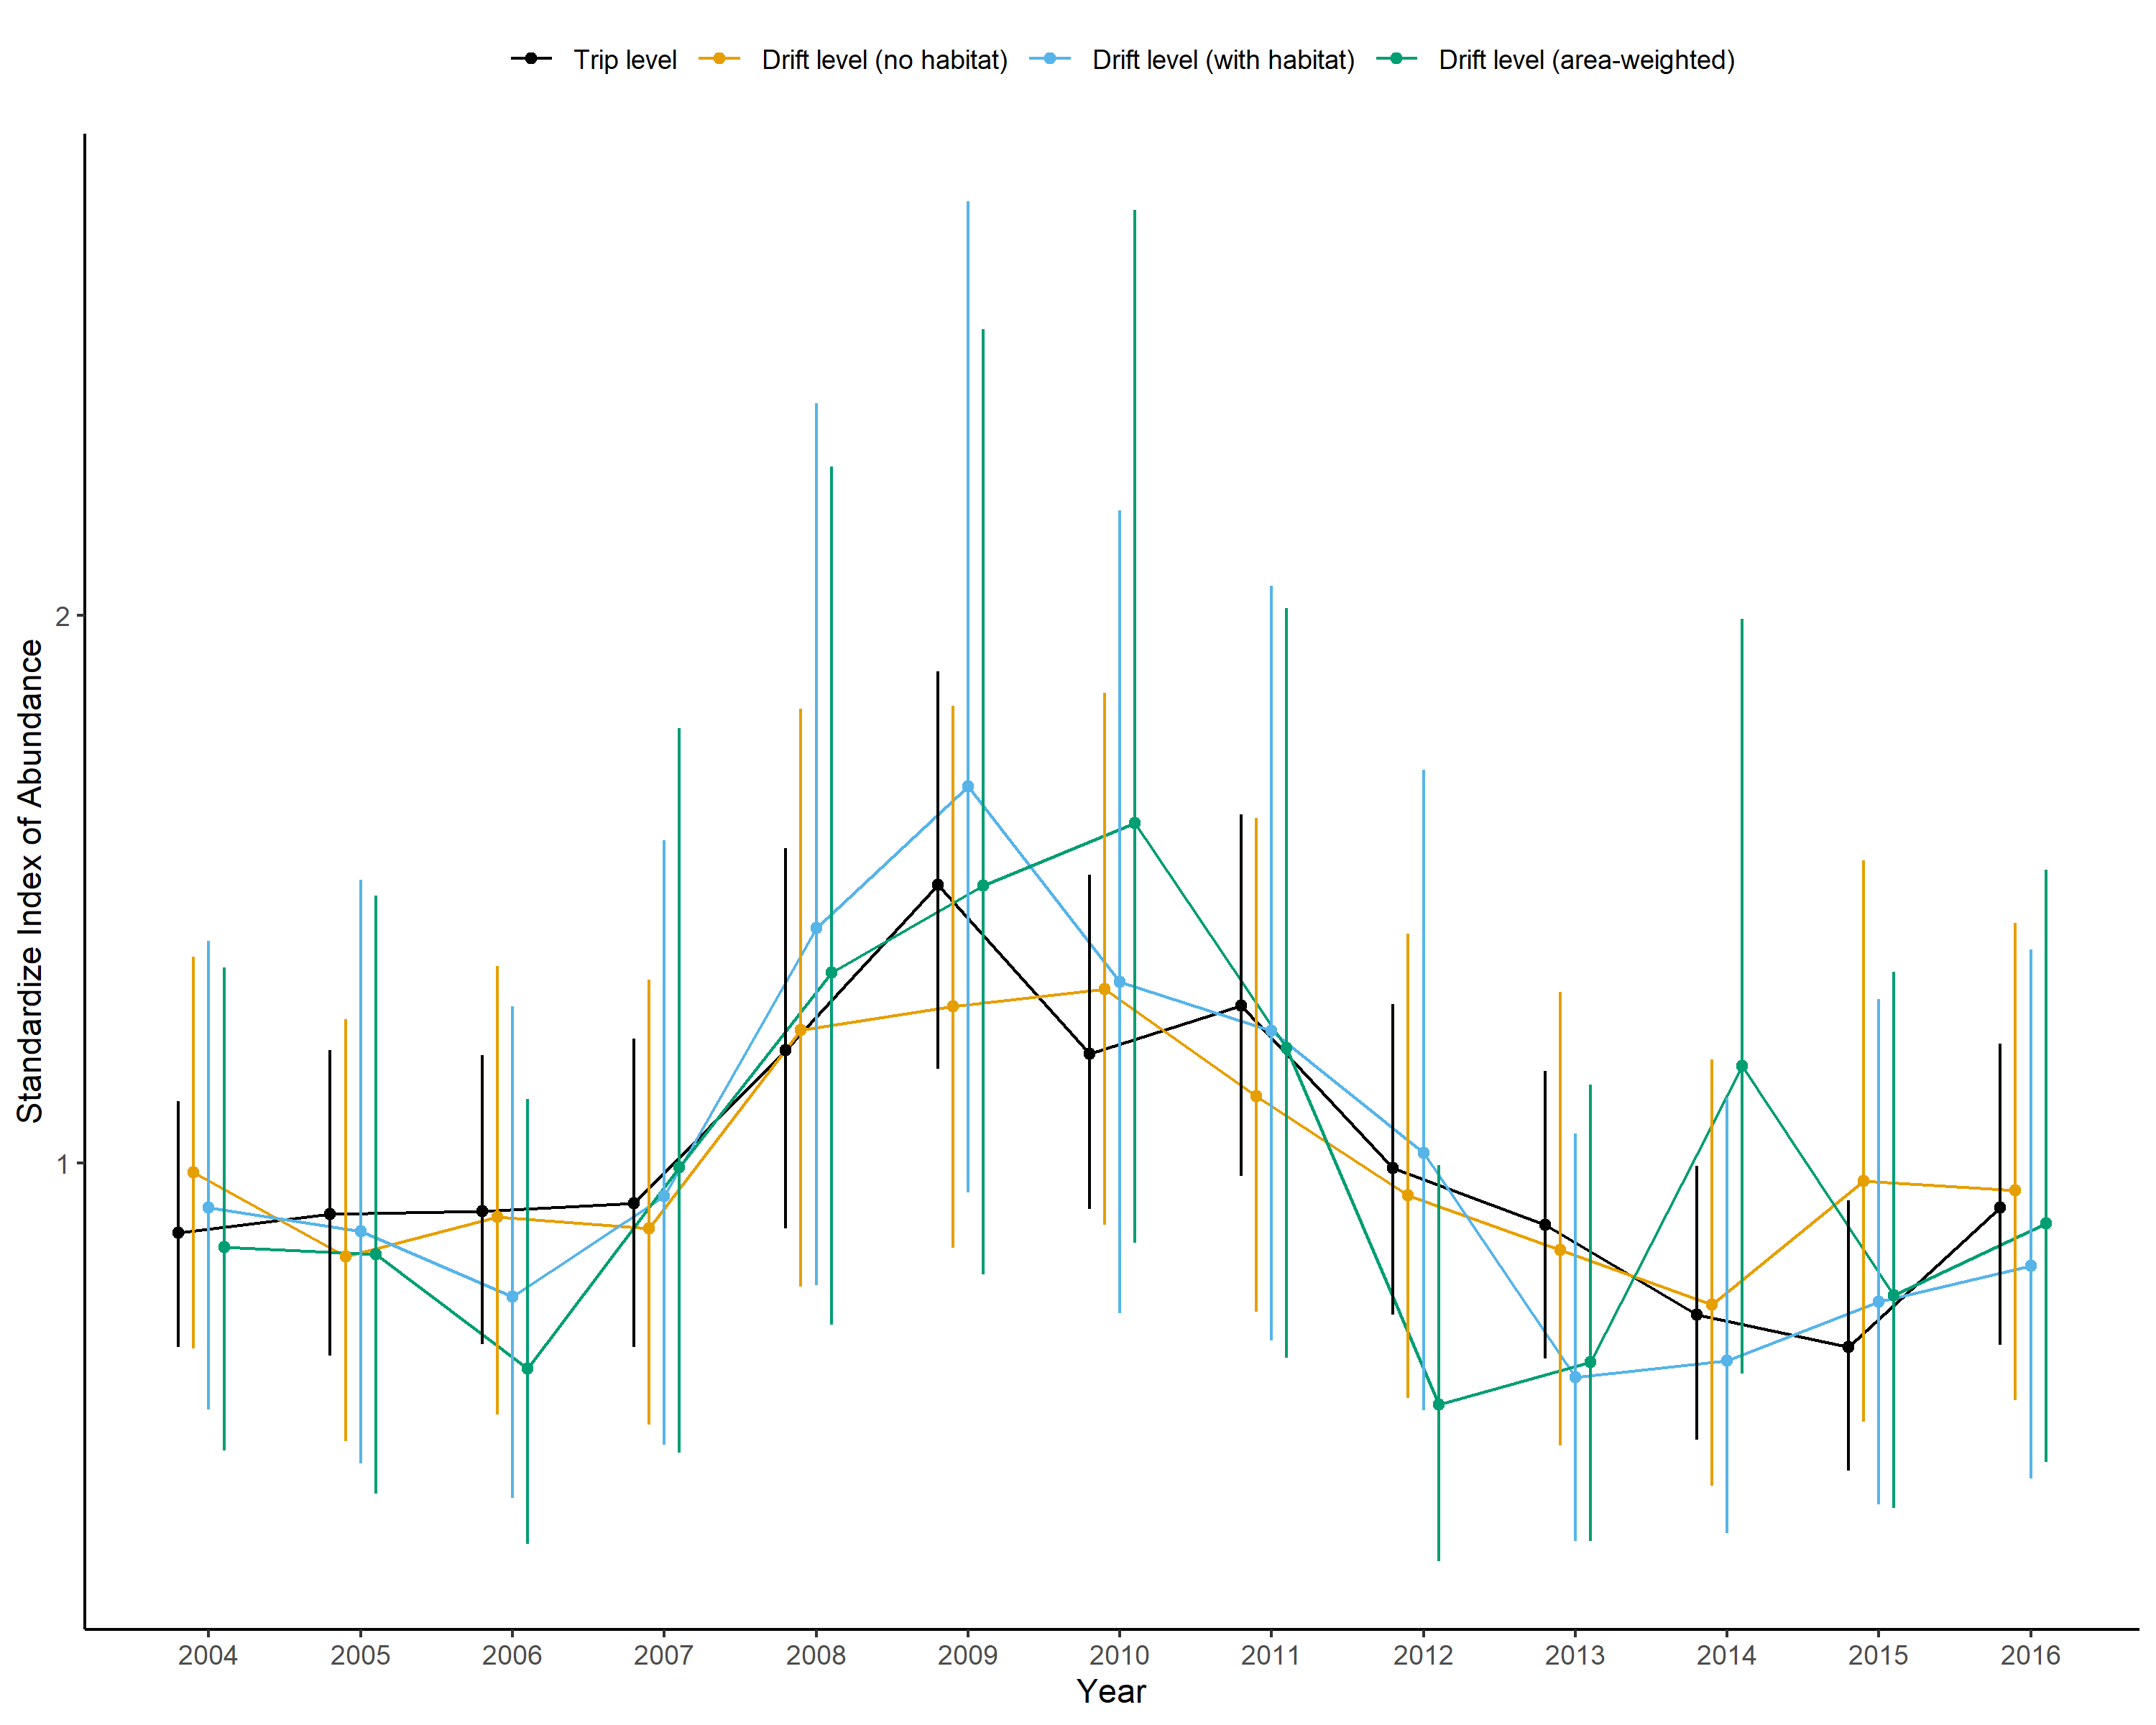
\includegraphics[width=3in,height=\textheight]{figures/china_indices.png}

}

\caption{\label{fig-china-indices}China rockfish}

}

\end{minipage}%
\newline
\begin{minipage}[t]{0.50\linewidth}

{\centering 

\raisebox{-\height}{

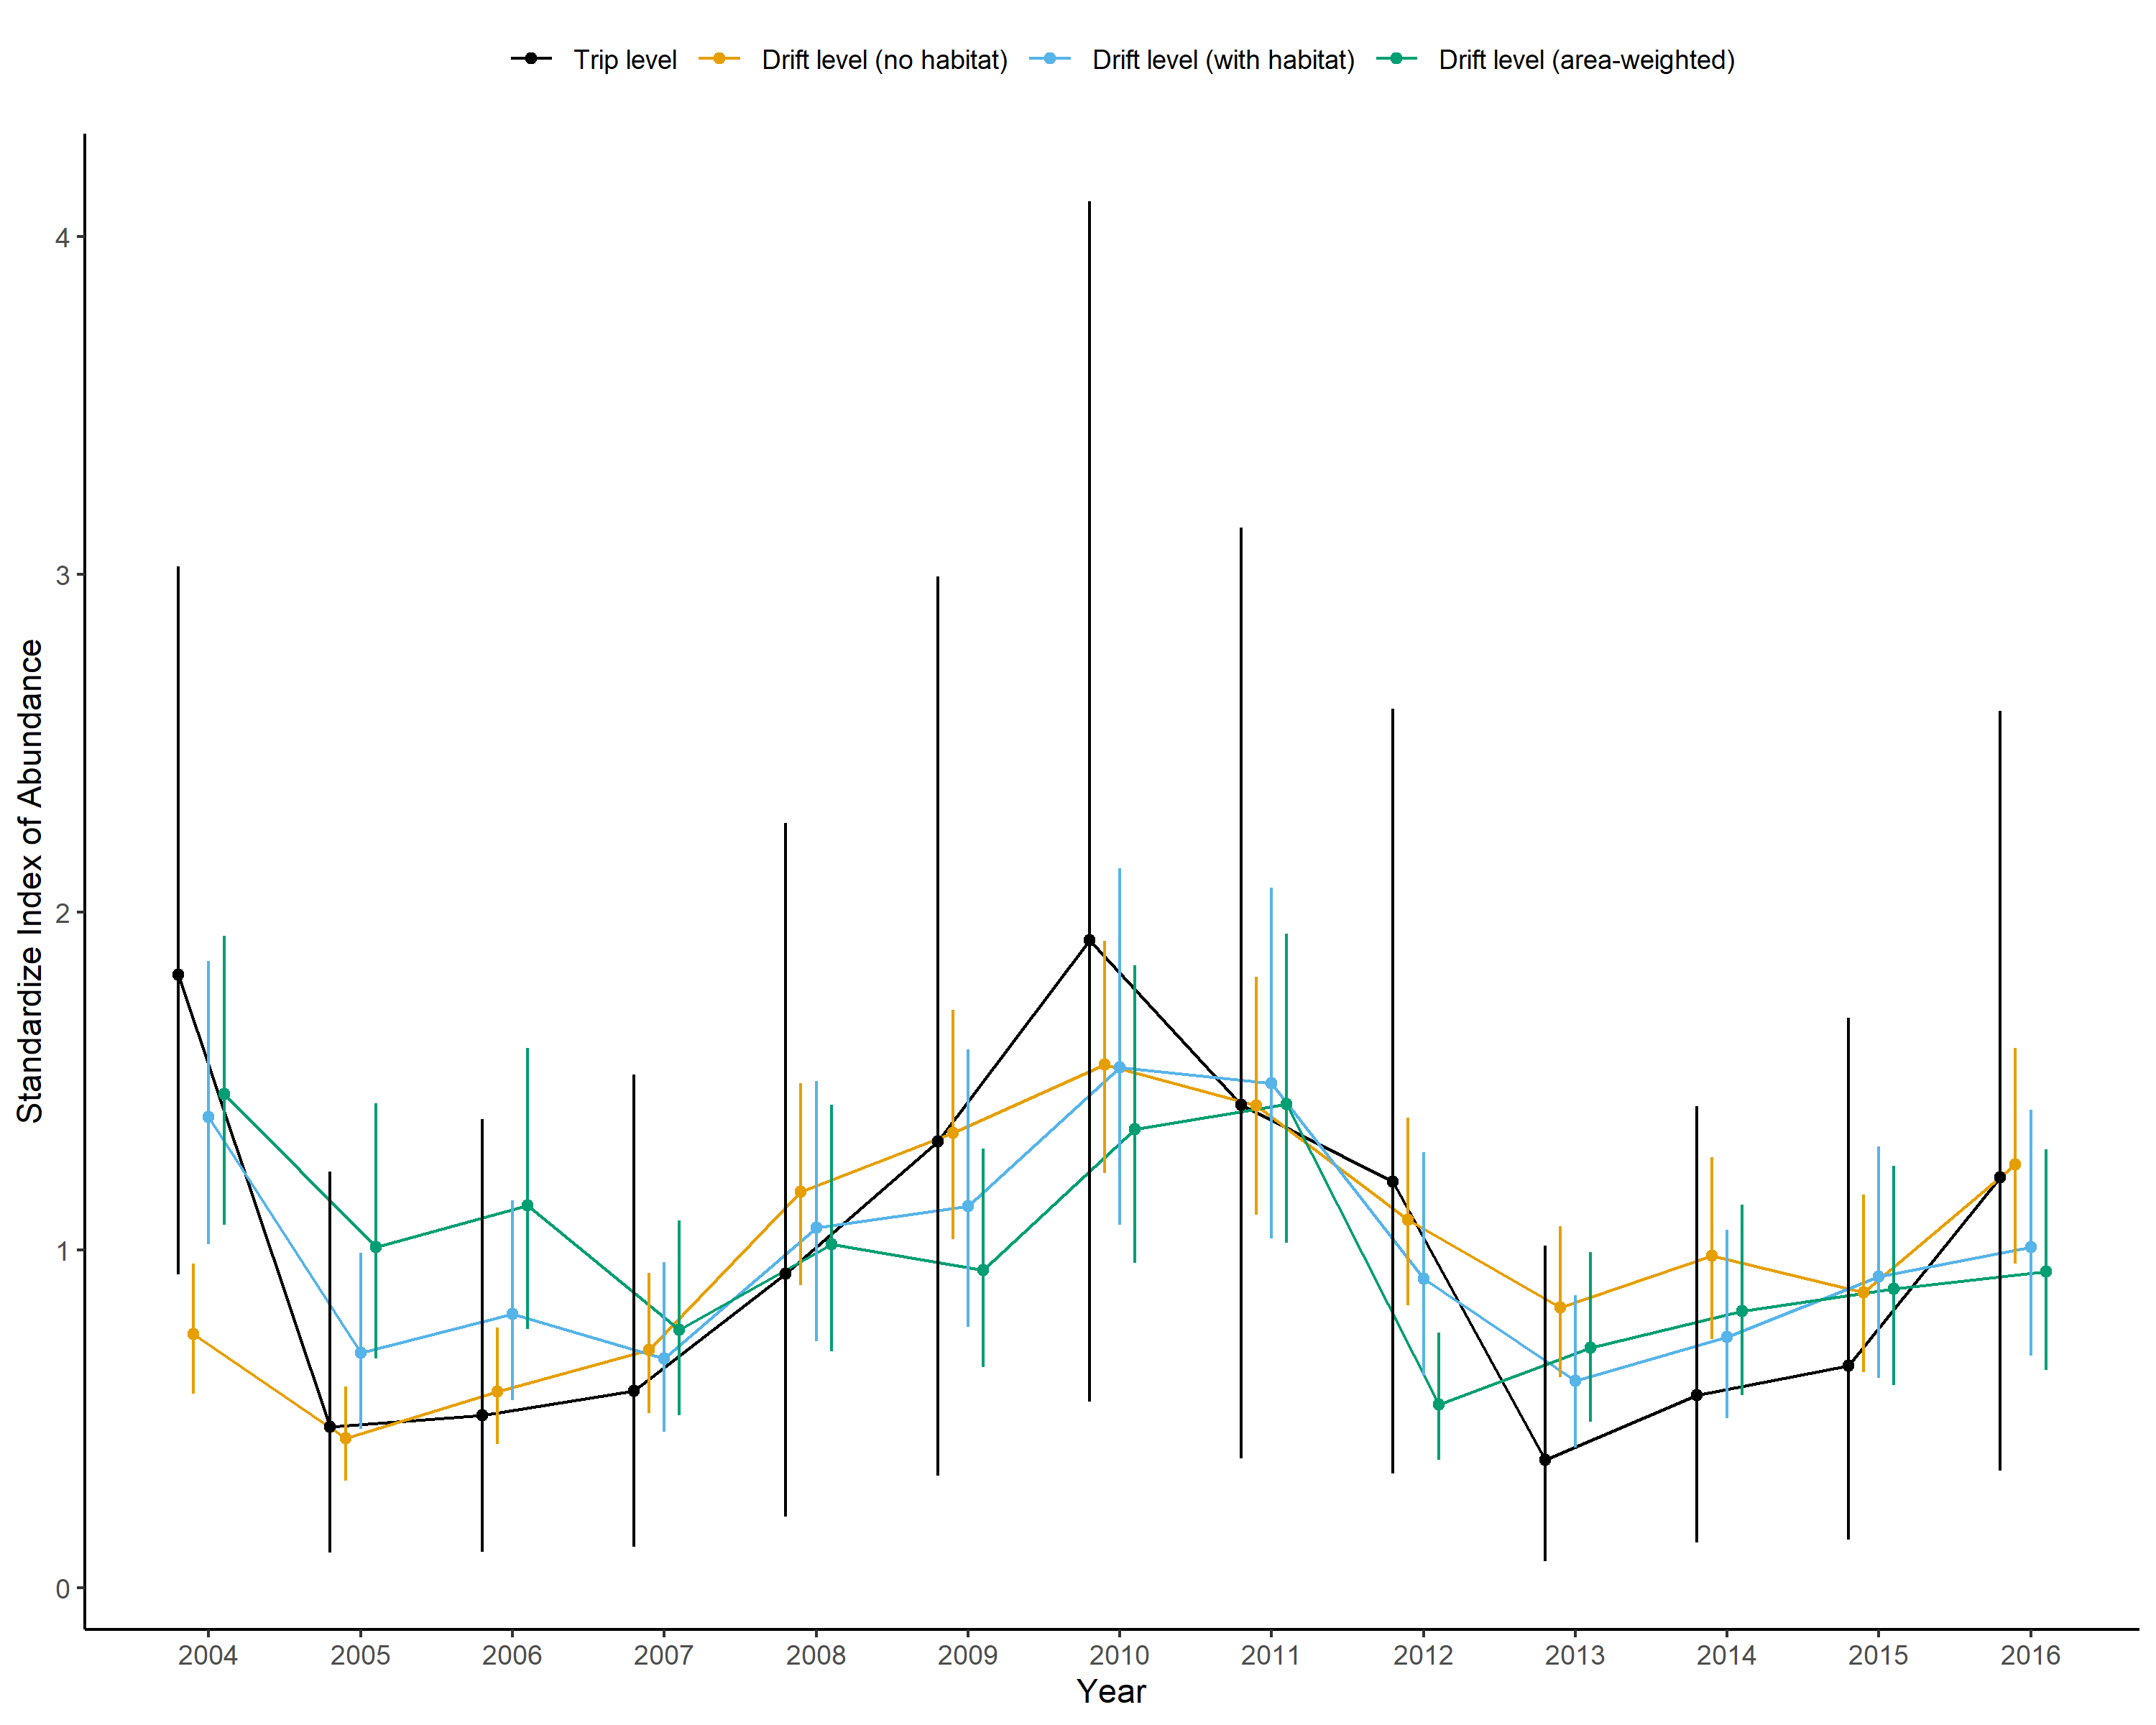
\includegraphics[width=3in,height=\textheight]{figures/gopher_indices.png}

}

\caption{\label{fig-gopher-indices}Gopher rockfish}

}

\end{minipage}%
%
\begin{minipage}[t]{0.50\linewidth}

{\centering 

\raisebox{-\height}{

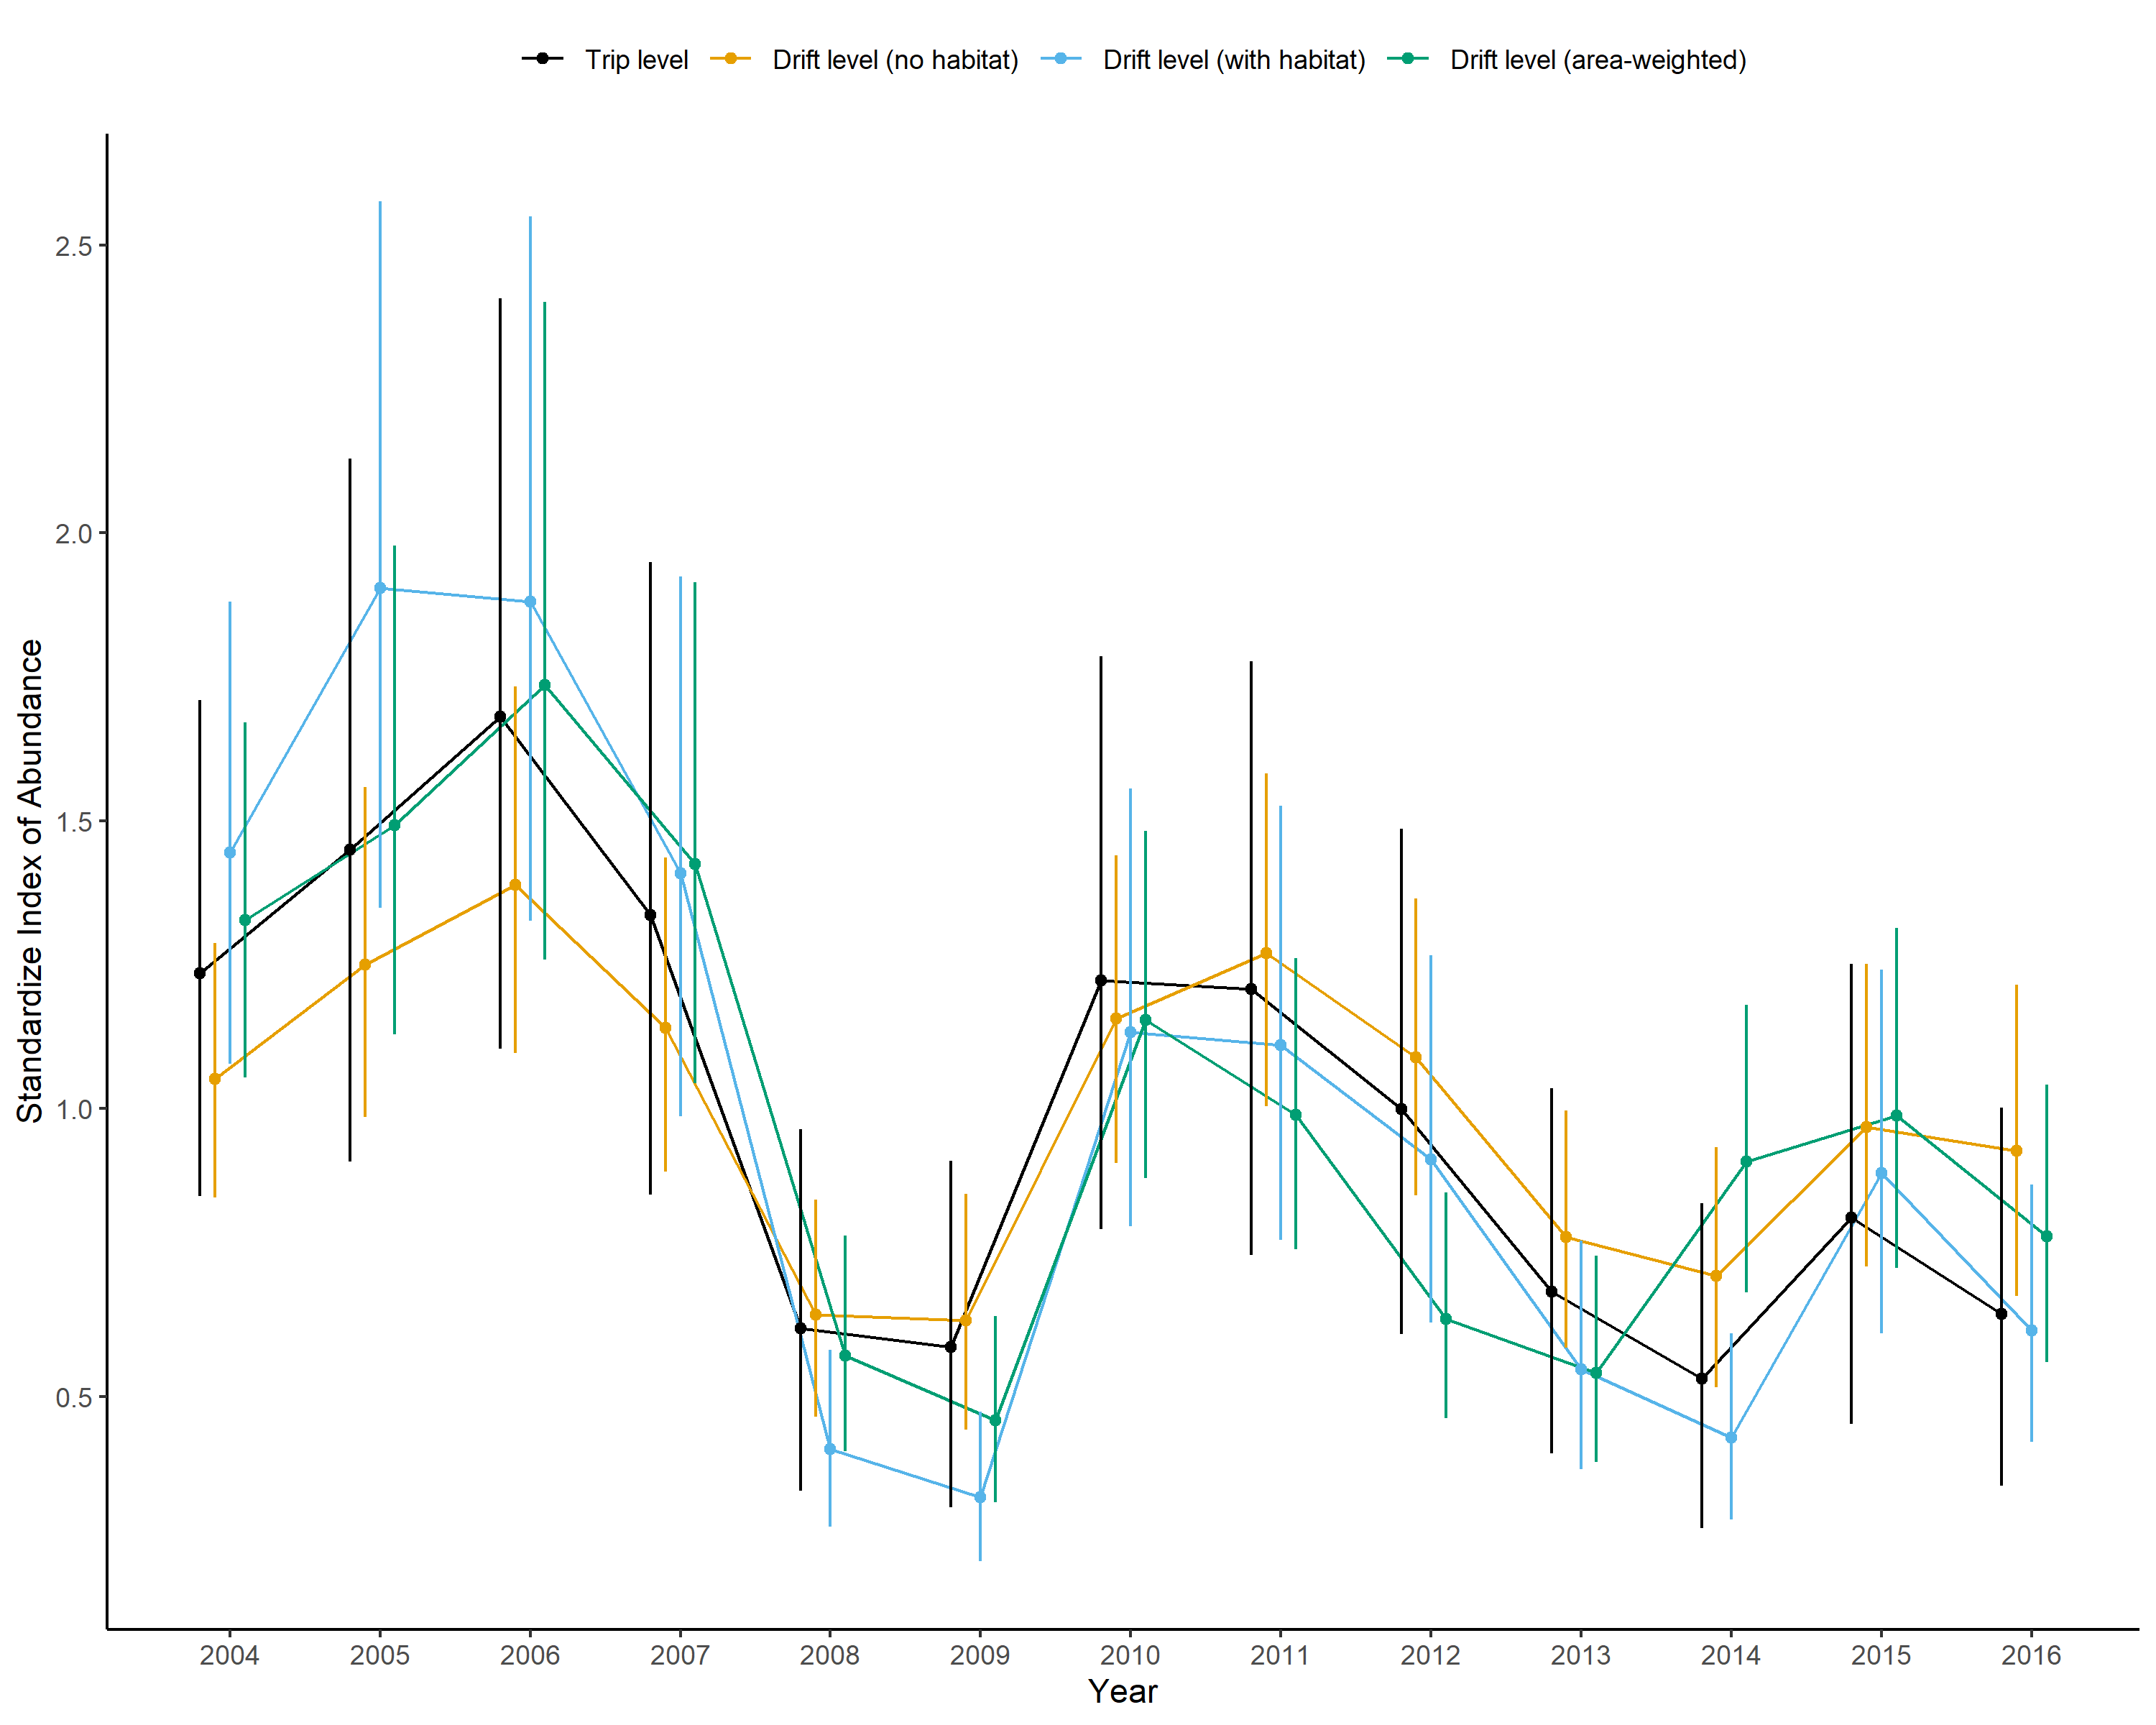
\includegraphics[width=3in,height=\textheight]{figures/vermilion_indices.png}

}

\caption{\label{fig-vermilion-indices}Vermilion rockfish}

}

\end{minipage}%
\newline
\begin{minipage}[t]{0.50\linewidth}

{\centering 

Indices of abundance for four iterations\ldots{}

}

\end{minipage}%

\end{figure}

\FloatBarrier


  \bibliography{bibliography.bib}


\end{document}
